%%%%%%%%%%%%%%%%%%%%%%%%%%%%%%%%%%%%%%%%%%%%%%%%%%%%%%%%%%%%
%%% LIVECOMS ARTICLE TEMPLATE FOR BEST PRACTICES GUIDE
%%% ADAPTED FROM ELIFE ARTICLE TEMPLATE (8/10/2017)
%%%%%%%%%%%%%%%%%%%%%%%%%%%%%%%%%%%%%%%%%%%%%%%%%%%%%%%%%%%%
%%% PREAMBLE
\documentclass[9pt,bestpractices,pubversion]{livecoms}
% Use the 'onehalfspacing' option for 1.5 line spacing
% Use the 'doublespacing' option for 2.0 line spacing
% Use the 'lineno' option for adding line numbers.
% The 'bestpractices' option for indicates that this is a best practices guide.
% Omit the bestpractices option to remove the marking as a LiveCoMS paper.
% Please note that these options may affect formatting.

\usepackage{lipsum} % Required to insert dummy text
\usepackage[version=4]{mhchem}
\usepackage{siunitx}
\usepackage{url}
\DeclareSIUnit\Molar{M}
\usepackage[italic]{mathastext}
\graphicspath{{figures/}}

%%%%%%%%%%%%%%%%%%%%%%%%%%%%%%%%%%%%%%%%%%%%%%%%%%%%%%%%%%%%
%%% IMPORTANT USER CONFIGURATION
%%%%%%%%%%%%%%%%%%%%%%%%%%%%%%%%%%%%%%%%%%%%%%%%%%%%%%%%%%%%
\usepackage[colorinlistoftodos]{todonotes}
\usepackage[most]{tcolorbox}
\usepackage{enumitem,amssymb}
\usepackage{textgreek}
\usepackage{changepage}

%%%%%%%%%%%%%%%%%%%%%%%%%%%%%%%%%%%%%%%%%%%%%%%%%%%%%%%%%%%%
%%% Added to allow customisation of table of contents
%%%%%%%%%%%%%%%%%%%%%%%%%%%%%%%%%%%%%%%%%%%%%%%%%%%%%%%%%%%%
\usepackage{tocloft}
\usepackage{xcolor}
\usepackage{todonotes}

% Define custom commands for colored TOC entries
\newcommand{\tocgreen}[1]{\textcolor{green}{#1}}
\newcommand{\tocorange}[1]{\textcolor{orange}{#1}}
\newcommand{\tocred}[1]{\textcolor{red}{#1}}

% Define custom commands for TOC entries with comments
\makeatletter
\newcommand{\tocsectioncomment}[1]{%
  \addtocontents{toc}{%
    {\leftskip \cftsecindent\relax
     \advance\leftskip \cftsecnumwidth\relax
     \rightskip \@tocrmarg\relax
     \textit{#1}\protect\par}}%
  \textit{#1}\par}

% Command for subsection comments in TOC
\newcommand{\tocsubsectioncomment}[1]{%
  \addtocontents{toc}{%
    {\leftskip \cftsubsecindent\relax
     \advance\leftskip \cftsubsecnumwidth\relax
     \rightskip \@tocrmarg\relax
     \textit{#1}\protect\par}}%
  \textit{#1}\par}

% Command for subsubsection comments in TOC
\newcommand{\tocsubsubsectioncomment}[1]{%
  \addtocontents{toc}{%
    {\leftskip \cftsubsecindent\relax
     \advance\leftskip \cftsubsubsecnumwidth\relax
     \rightskip \@tocrmarg\relax
     \textit{#1}\protect\par}}%
  \textit{#1}\par}

\makeatother

%%%%%%%%%%%%%%%%%%%%%%%%%%%%%%%%%%%%%%%%%%%%%%%%%%%%%%%%%%%%

\newcommand{\versionnumber}{2.0} % you should update the minor version number in preprints and major version number of submissions.
\newcommand{\githubrepository}{\url{https://github.com/alchemistry/alchemical-best-practices}} %this should be the main github repository for this article
\newcommand{\expect}[1]{\left\langle{#1}\right\rangle}
%%%%%%%%%%%%%%%%%%%%%%%%%%%%%%%%%%%%%%%%%%%%%%%%%%%%%%%%%%%%
%%% ARTICLE SETUP
%%%%%%%%%%%%%%%%%%%%%%%%%%%%%%%%%%%%%%%%%%%%%%%%%%%%%%%%%%%%
\title{Best Practices for Single Alchemical Free Energy Calculations [Article v\versionnumber]}
\author[1*]{Antonia S. J. S. Mey}
\author[2]{Bryce K. Allen}
\author[3]{Hannah E. Bruce Macdonald}
\author[3*]{John D. Chodera}
\author[9]{David F. Hahn}
\author[1,10]{Maximilian Kuhn}
\author[1]{Julien Michel}
\author[4*]{David L. Mobley}
\author[5]{Levi N. Naden}
\author[6]{Samarjeet Prasad}
\author[2,7]{Andrea Rizzi}
\author[1]{Jenke Scheen}
\author[8*]{Michael R. Shirts}
\author[9]{Gary Tresadern}
\author[2]{Huafeng Xu}
%
\affil[1]{EaStCHEM School of Chemistry, David Brewster Road, Joseph Black Building, The King's Buildings, Edinburgh, EH9 3FJ, UK}
\affil[2]{Silicon Therapeutics, Boston, MA, USA}
\affil[3]{Computational and Systems Biology Program, Sloan Kettering Institute, Memorial Sloan Kettering Cancer Center, New York NY, USA}
\affil[4]{Departments of Pharmaceutical Sciences and Chemistry, University of California, Irvine, Irvine, USA}
\affil[5]{Molecular Sciences Software Institute, Blacksburg VA, USA}
\affil[6]{National Institutes of Health, Bethesda, MD, USA}
\affil[7]{Tri-Institutional Training Program in Computational Biology and Medicine, New York, NY, USA}
\affil[8]{University of Colorado Boulder, Boulder, CO, USA}
\affil[9]{Computational Chemistry, Janssen Research \& Development, Turnhoutseweg 30, Beerse B-2340, Belgium}
\affil[10]{Cresset, Cambridgeshire, UK}

%
\corr{antonia.mey@ed.ac.uk}{ASJSM}
\corr{john.chodera@choderalab.org}{JDC}
\corr{dmobley@mobleylab.org}{DLM}
\corr{michael.shirts@colorado.edu}{MRS}

\orcid{Antonia S. J. S. Mey}{0000-0001-7512-5252}
\orcid{Bryce Allen}{0000-0002-0804-8127}
\orcid{Hannah E. Bruce Macdonald}{0000-0002-5562-6866}
\orcid{John D. Chodera}{0000-0003-0542-119X}
\orcid{Maximilian Kuhn}{0000-0002-2811-3934}
\orcid{Julien Michel}{0000-0003-0360-1760}
\orcid{David L. Mobley}{0000-0002-1083-5533}
\orcid{Levi N. Naden}{0000-0002-3692-5027}
\orcid{Samarjeet Prasad}{0000-0001-8320-6482}
\orcid{Andrea Rizzi}{0000-0001-7693-2013}
\orcid{Jenke Scheen}{0000-0001-9781-0445}
\orcid{Michael R. Shirts}{0000-0003-3249-1097}
\orcid{Gary Tresadern}{0000-0002-4801-1644}
\orcid{Huafeng Xu}{0000-0001-5447-0452}
\orcid{David F. Hahn}{0000-0003-2830-6880}

\blurb{This LiveCoMS document is maintained online on GitHub at \githubrepository; to provide feedback, suggestions, or help improve it, please visit the GitHub repository and participate via the issue tracker.}

%%%%%%%%%%%%%%%%%%%%%%%%%%%%%%%%%%%%%%%%%%%%%%%%%%%%%%%%%%%%
%%% PUBLICATION INFORMATION
%%% Fill out these parameters when available
%%% These are used when the "pubversion" option is invoked
%%%%%%%%%%%%%%%%%%%%%%%%%%%%%%%%%%%%%%%%%%%%%%%%%%%%%%%%%%%%
\pubDOI{10.33011/livecoms.2.1.18378}
\pubvolume{2}
\pubyear{2020}
\articlenum{18378}
\datereceived{5 August 2020}
\dateaccepted{25 November 2020}

%%%%%%%%%%%%%%%%%%%%%%%%%%%%%%%%%%%%%%%%%%%%%%%%%%%%%%%%%%%%
%%% ARTICLE START
%%%%%%%%%%%%%%%%%%%%%%%%%%%%%%%%%%%%%%%%%%%%%%%%%%%%%%%%%%%%
\begin{document}

\begin{frontmatter}
\maketitle
%%%%%%%%%%%%%%%%%%%%%%%%%%%%%%%%%%%%%%%%%%%%%%%%%%%%%%%%%%%%
%%% Abstract
%%%%%%%%%%%%%%%%%%%%%%%%%%%%%%%%%%%%%%%%%%%%%%%%%%%%%%%%%%%%
\begin{abstract}


\todo[inline, color=green!20]{
    
The original best practices guide will be split into two documents: the first will gives best practices for running a \emp{single} calculation (and cover theory in more depth/ detail system-specific setup etc.), while the second will give best practices for running \emp{multiple} calculations (with a focus on automation). The first will become version 2.0 of the current guide, while the second will be submitted as a new manuscript.

This document outlines the contents of the first document for single calculations.
}

\todo[inline, color=green!20]{@Volunteer Update abstract to highlight the split of the document and focus on the single calculations.}

Alchemical free energy calculations are a useful tool for predicting free energy differences associated with the transfer of molecules from one environment to another.
The hallmark of these methods is the use of "bridging" potential energy functions representing \emph{alchemical} intermediate states that cannot exist as real chemical species. The data collected from these bridging alchemical thermodynamic states allows the efficient computation of transfer free energies (or differences in transfer free energies) with orders of magnitude less simulation time than simulating the transfer process directly. 
While these methods are highly flexible, care must be taken in avoiding common pitfalls to ensure that computed free energy differences can be robust and reproducible for the chosen force field, and that appropriate corrections are included to permit direct comparison with experimental data.

In this paper, we review current best practices for several popular application domains of  alchemical free energy calculations performed with equilibrium simulations, in particular relative and absolute small molecule binding free energy calculations to biomolecular targets.

% \todo[inline, color=green!20]{JDC: Should we migrate this document to \url{https://github.com/alchemistry}? ASJSM: Let's migrate with the submitted version, but leave it here for now?}
\end{abstract}
\end{frontmatter}

\newpage
% Add a comment to the top of the contents page
\addtocontents{toc}{\vskip2pt\noindent\textcolor{green}{\textbf{Green sections}: Minimal revisions required}\par\vskip2pt}
\addtocontents{toc}{\vskip2pt\noindent\textcolor{orange}{\textbf{Orange sections}: Substantial revisions required}\par\vskip2pt}
\addtocontents{toc}{\vskip2pt\noindent\textcolor{red}{\textbf{Red sections}: Needs written from scratch.}\par\vskip2pt}

\tableofcontents

\newpage

%%%%%%%%%%%%%%%%%%%%
%  Introduction    %
%%%%%%%%%%%%%%%%%%%%

\section{\tocgreen{What are alchemical free energy methods?}}
\tocsectioncomment{Steering Meeting: @Jenke Scheen to think about how figure can be made the "central axis" of the paper. Possibly update/ create new full-page figure and expand so that it shows a ``dummy workflow'' for an alchemical simluation including all general stages (e.g setup, analysis with different estimators etc.), and guides readers to appropriate sections.}
\label{sec:intro}
Alchemical free energy calculations compute free energy differences associated with transfer processes, such as the binding of a small molecule to a receptor, the transfer of a small molecule from an aqueous to apolar phase~\cite{zwanzig1954hightemperature}, or the effects of protein side chain mutations on binding affinities or thermostabilities. 
 These calculations use non-physical\footnote{Here, the non-physical nature of the transformation is referred to as "alchemical", a term coined by Tembre and McCammon in Ref.~\cite{tembre1984ligandreceptor}.} intermediate states in which the chemical identity of some portion of the system (such as a small molecule ligand or protein sidechain) is changed by modifying the potential governing the interactions with the environment for the atoms being modified, inserted, or deleted. 

Fig.~\ref{fig:fig_what_is_alchemy} illustrates common free energy changes that may be difficult to compute with unbiased molecular dynamics methods, but are more tractable with alchemical methods.
In alchemical simulations, the introduction of intermediate \textit{alchemical states} that bridge the high-probability regions of configuration space between two physical endstates of interest, permits the robust computation of free energy for large transformations.
Alchemical calculations can be used in a variety of scenarios, such as: 
\begin{itemize}
\item computing the free energy of a conformational change for a molecule with a high barrier to interconversion (Fig.~\ref{fig:fig_what_is_alchemy}\textbf{A});
\item computing partition ($\log P$) or distribution ($\log D$) coefficients between environments (Fig.~\ref{fig:fig_what_is_alchemy}\textbf{B})~\cite{rustenburg2016measuring, bosisio2016blinded} 
\item determining partitioning between compartments into membranes (Fig.~\ref{fig:fig_what_is_alchemy}\textbf{C})~\cite{corey2019insights}. 
\end{itemize}

Furthermore, alchemical calculations are frequently used to estimate changes in free energies upon modifying a ligand or protein: 
\begin{itemize}
\item a protein residue can be alchemically mutated to probe the impact on binding affinity (Fig.~\ref{fig:fig_what_is_alchemy}\textbf{D})\cite{hauser2018predicting,aldeghi2018accurate} or changes in protein thermostability~\cite{seeliger2010protein,gapsys2016insights,gapsys2016accurate,aldeghi2019accurate}; 
\item the entire ligand can be alchemically transferred from protein to solvent in an absolute binding free energy calculation (Fig.~\ref{fig:fig_what_is_alchemy}\textbf{E})~\cite{mobley2007predicting,aldeghi2015accurate,aldeghi2017predictions}; 
\item small alchemical modifications can be made between chemically related ligands to estimate relative differences in binding free energies (Fig.~\ref{fig:fig_what_is_alchemy}\textbf{F})~\cite{wang2015accurate,mey2016blinded,song2019using,gapsys2020large,kuhn2020assessment}.
\end{itemize}


After an alchemical calculation is performed, which generally involves multiple simulations at a variety of alchemical states, the data must be analyzed to compute an estimate of the free energy for the transformation of interest.
 Early work used simple but statistically suboptimal estimators for this: free energy perturbation (FEP) used a simple (but highly biased) estimator based on the Zwanzig relation~\cite{zwanzig1954hightemperature} or numerical quadrature via thermodynamic integration (TI), for which the theory dates back the better part of a century but with the first computational applications emerging in the 1980's and 90's~\cite{kirkwood1935statistical, jorgensen1985monte, kollman1993free, wong1986dynamics, merz1989free}. %
 More recent developments have seen new, highly efficient statistical estimators that make better use of all the data, often building on the more efficient and less biased Bennett acceptance ratio (BAR)~\cite{bennett1976efficient}, producing multistate generalizations~\cite{shirts2008statisticallya} or removing the need for global equilibrium~\cite{wu2016multiensemble, mey2014xtram, wu2014statistically}.

Subsequent work in the 2000s led to improved implementations of alchemical methods in popular biomolecular simulation packages~\cite{shirts2003extremely,shirts2005solvation,vanderspoel2005gromacs, mermelstein2018fast, wang2015accurate, hedges2019biosimspace, riniker2011calculation}. 
 This foundational work, combined with the methodological, technological, and hardware improvements of the last 5--10 years, has led to an explosion of interest and direct commercial application of these technologies~\cite{wang2015accurate, fratev2019improved, schindler2020largescale, cournia2017relative, sherborne2016collaborating, kuhn2020assessment}.


As the field of molecular simulation can now routinely access microsecond timescales with the aid of GPUs~\cite{salomon-ferrer2013routine}, and millisecond timescales appear to soon be within reach, accurate alchemical calculations on even more challenging problems will become reasonable to perform. 
In the meantime, today's users may find it difficult to get started with these complex calculations whilst also keeping up with the fast pace of change. 
This Best Practices guide provides current recommendations and tips for users of all experience. Updates and suggestions are welcomed via our GitHub repository at \url{https://github.com/alchemistry/alchemical-best-practices}.    

\begin{figure}
    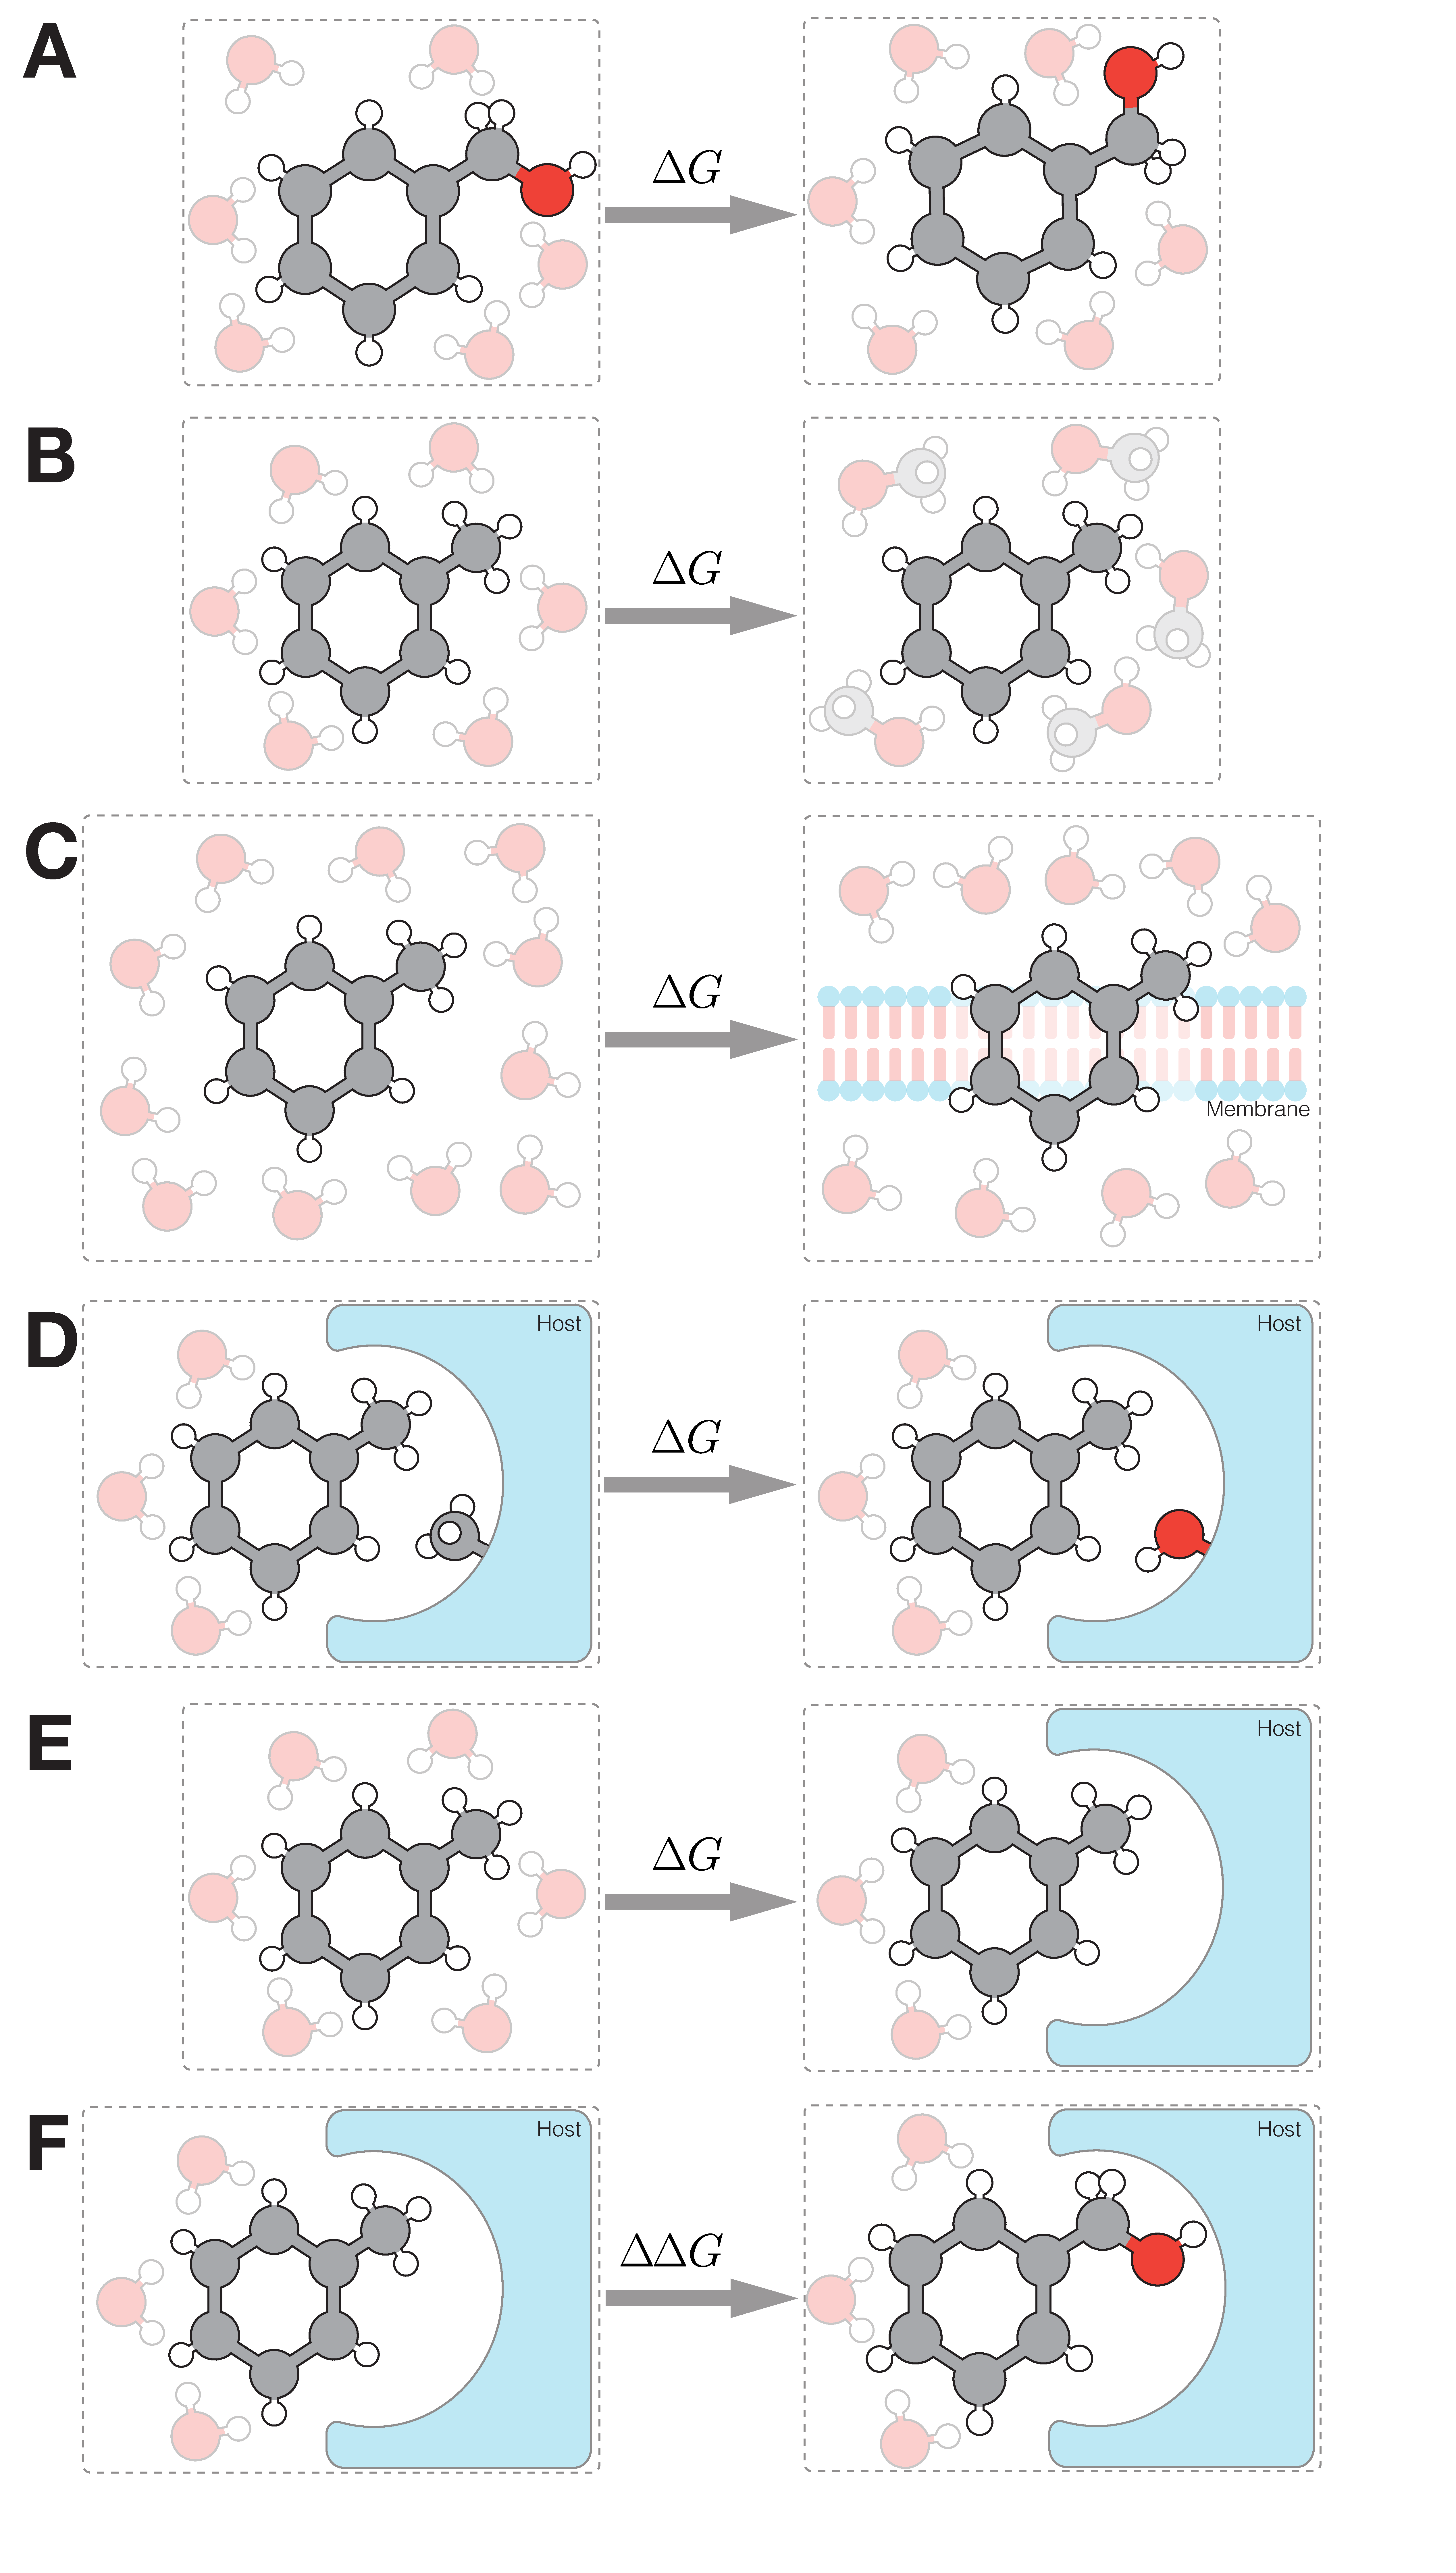
\includegraphics[width=0.95\linewidth]{figures/fig1_what_is_alchemy/Figure.pdf}   
    \caption{\textbf{Illustration of common types of free energies differences that can be calculated using alchemical free energy methods.} \textbf{A}: Change in free energy due to a conformational change of the molecule across a high barrier. \textbf{B}: Partition coefficient such as $\log P$ or $\log D$ depend on a change in free energy between different phases; here, as an example the partition coefficient between methanol and water is shown. \textbf{C}: Free energy difference associated with the insertion of a molecule into a membrane. \textbf{D}: Effect of mutations of protein or host residues on free energies of binding. \textbf{E}: Relative free energy of binding of one molecule with respect to another, here toluene and benzyl alcohol, \textbf{F}: absolute free energies of binding of a small molecule to a host (e.g. protein).
    \label{fig:fig_what_is_alchemy}
    }
\end{figure}

%%%%%%%%%%%%%%%%%%%%
% Prerequesites    %
%%%%%%%%%%%%%%%%%%%%
\section{\tocorange{Prerequisites and Scope}}
\tocsectioncomment{Steering Meeting: @Volunteer to update reflecting new split between single and multiple calculations. @Michael Shirts to update best practices on multiple binding sites.}
\label{sec:pre}

This Best Practices guide focuses on providing a good starting point for new practitioners and a reference for experienced practitioners. 
 For this purpose we provide a convenient checklist (Sec.~\ref{sec:checklist}) to help ensure all calculations comply with currently-understood best practices for alchemical simulation and analysis. Where the best practices are currently not certain, we highlight areas where further research is needed to identify an unambiguous recommendation.
 This guide can also serve as a set of best practices to ensure simulation robustness and reproducibility which reviewers may wish to consider as they evaluate papers.

 We assume that novice practitioners have at least moderate experience with molecular simulation concepts and use of simulation packages. 
 Furthermore, basic familiarity with the principles of molecular mechanics, molecular dynamics simulations, statistical mechanics, and the biophysics of protein-ligand association are essential. If you feel unfamiliar with some of these concepts, good starting points can be found in these references~\cite{braun2019best, grossfield2018best, klimovich2015guidelines, shirts2012best}. 

 While reading this Best Practices guide, it is important to bear in mind \emph{this is not a review} of all free energy calculation methods at the cutting edge of current research.
Instead this guide aims to answer the following questions:
\begin{itemize}
    \item Is my problem suitable for an alchemical calculation? 
     \item How do I select an appropriate alchemical protocol? 
     \item What software tools are available to perform alchemical calculations? 
     \item How should I analyze my data and report uncertainties? 
\end{itemize}


Some other background information may be needed depending on the nature of the alchemical project. For example, often, if binding poses are not known, docking calculations can be used to generate an initial small molecule binding pose to start alchemical simulations. This will require some basic familiarity on how to perform docking to generate reasonable simulation starting points~\cite{grinter2014challenges}. 

As some of the theoretical background can seem daunting, we do, however, provide a guide to the essential theory behind alchemical free energy calculations in Sec.~\ref{sec:theory}.
In the remainder of this paper, we will cover topics that are key to the preparation (Sec.~\ref{sec:prerequisites}), choice and use of correct protocols (Sec.~\ref{sec:simulation_protocol_choice}), and finally the best practices that should be used in the analysis of alchemical calculations (Sec.~\ref{sec:data_analysis}). 
Particular focus will be given to aspects of the molecular simulations which are unique to alchemical calculations---these include the calculation of transfer free energies (hydration free energies, partition coefficients, etc.), and binding free energies (absolute and relative). We primarily focus on free energy calculations using simulations performed at \emph{equilibrium} in this Best Practices guide, as best practices for these are more developed, and non-equilibrium techniques may warrant their own guide as such practices evolve. 


While we try to address as many methods and practices as possible, the field of free energy calculations is broad, and there are many advanced topics that are left to future Best Practices documents focusing on specific issues. 
Below, we provide a non-exhaustive list of topics we have \emph{not} addressed, along with some references to provide starting points on these more advanced topics:
\begin{itemize}
\item covalent inhibition~\cite{lameira2019predicting}
\item free energies of mutation of protein side chains~\cite{gapsys2016accurate,aldeghi2018accurate}
\item nonspecific binding or multiple binding sites~\cite{gill2018binding}
\item approximate and often less accurate endpoint free energy methods such as MM-PBSA~\cite{genheden2015mm} and LIE~\cite{gutierrez-de-teran2012linear}
\item Free energy methods that extract the ligand using geometric order parameters and potential of mean force methods~\cite{heinzelmann2017attachpullrelease}
\item forcefield dependence for protein, ligand, ions, co-solvents, and co-factors. A number of different studies have looked at the influence of force fields and it is assumed the user has made an appropriate choice for the system under study~\cite{loeffler2018reproducibility, vassetti2019assessment, lopes2015current}. 
\item non-equilibrium free energy calculations~\cite{gapsys2020large}
\item Free energy calculations using QM/MM methods~\cite{beierlein2011simple,dybeck2016comparison,cave-ayland2015direct}.
\item Free energy calculations using machine learning methods~\cite{rufa2020chemical, scheen2020hybrid, cole2020machine}
\end{itemize}

For convenience we have also compiled a list of common acronyms and common symbols used throughout this paper.
\begin{tcolorbox}[title=Acronyms, colback=blue!10!white]
    {\bf CPU} --- Central Processing Unit\\
     {\bf BAR} --- Bennett Acceptance Ratio\\
     {\bf FEP} --- Free Energy Perturbation\\
     {\bf GPCR} --- G-Protein Coupled Receptor\\
     {\bf GPU} --- Graphics Processing Unit\\
     {\bf MBAR} --- Multistate Bennett Acceptance Ratio\\
     {\bf MCSS} --- Maximum Common Substructure\\
     {\bf MD} --- Molecular Dynamics\\
     {\bf RMSE} --- Root Mean Square Error\\
     {\bf MUE} --- Mean Unsigned Error\\
     {\bf SAR} --- Structure-Activity Relationships\\
     {\bf TI} --- Thermodynamic Integration
\end{tcolorbox}


\begin{tcolorbox}[title=List of Symbols, colback=green!10!white]
$L$ and $R$ --- generic names for ligand and receptor\\
$K_b^{\circ}$ --- binding  constant \\
$c^{\circ}$ --- standard state concentration \\
$U$ --- potential energy\\
$u$ --- reduced (dimensionless) potential describing a thermodynamic state \\
$G$ --- Gibbs free energy (free energy in the isothermal isobaric ensemble), Gibbs function, or free enthalpy, though the most common term Gibbs free energy is used in the text\\
$A$ --- Helmholtz free energy (free energy in the canonical ensemble) or Helmholtz function, with Helmholtz free energy used in the text.\\
$f$ --- reduced (dimensionless) free energy \\
$\Delta \hat{f}$ --- estimate from an estimator for the reduced free energy difference between two states\\
$\Gamma$ --- configurational space accessible by simulations \\
$\vec{q}$ --- vector of a single configuration, i.e. $x$, $y$, $z$ coordinates of the simulation system\\
$k_B$ --- Boltzmann constant \\
$Z$ --- partition function \\
$p$ --- pressure \\
$\mu$ --- chemical potential (grand canonical ensemble)\\
$T$ --- temperature \\
$\beta \equiv (k_B T)^{-1}$ --- inverse thermal energy \\
$\vec{\lambda}$ --- alchemical progress parameter, which may be multidimensional \\
$g$ --- statistical inefficiency\\
$\mathcal{O}$ --- overlap matrix\\
$C_t$ --- discrete-time-normalized fluctuation auto-correlation function\\
$\tau _{eq}$ --- integrated auto-correlation time\\
$t_0$ --- equilibration time
\end{tcolorbox}

%%%%%%%%%%%%%%%%%%%%
% Theory basics    %
%%%%%%%%%%%%%%%%%%%%
\section{\tocorange{Statistical mechanics demonstrates why alchemical free energy calculations work}}
\tocsectioncomment{Steering Meeting: @Emilio Gallicchio to update theory. Will frame it to be as general as possible, while remaining accessible to beginners. Will align with Gilson et al. 1997 paper. @Darrin York to review.}
\label{sec:theory}

Why would you want to run an alchemical free energy calculation and why do they work?
In this section, we use the example of relative free energy calculations to sketch the theory of alchemical simulations and illustrate their utility.
The emphasis here is placed on bridging theoretical foundations and intuition.
A rigorous derivation of the standard (absolute) free energy of binding using the principles of statistical mechanics can be found in Gilson's classic work~\cite{gilson1997statisticalthermodynamic}.

\subsection{Simulating binding events of receptor-drug systems can be computationally expensive}
Suppose you want to compute the binding affinity, or free energy of binding, of a ligand $L$ to a receptor $R$, given by:
\begin{equation}
R+L \leftrightharpoons RL.
\end{equation}
The binding constant ($K_b^{\circ}$) is given by the law of mass action as the ratio of concentrations of product $[RL]$ and reactants $[R]$, $[L]$:
\begin{equation}\label{eq:law-mass-action}
 K_b^{\circ} = c^{\circ}\frac{[RL]}{[L][R]}.
\end{equation}
The standard state concentration $c^\circ$ depends on the reference state, but it is usually set to $1\,\mathrm{mol}/\mathrm{L}$ assuming a constant pressure of $1\,\mathrm{atm}$ (see also Sec.~\ref{sec:standardstate-restraints}). Eq.~\ref{eq:law-mass-action} also holds for dilute solutions if thermodynamic activities can be approximated by concentrations~\cite{gilson1997statisticalthermodynamic}.
Thus, the standard Gibbs free energy of binding $\Delta G_{\mathrm{bind}}$ is given by:
\begin{equation}
    \Delta G_{\mathrm{bind},L} = -k_BT\ln K_b^{\circ},
\end{equation}
where $k_B$ is the Boltzmann constant and $T$ the temperature of the system.
Note that, unless otherwise specified, we use $\Delta G$ throughout the paper to refer to the \textit{standard} free energy of binding (or solvation) (see also Sec.~\ref{sec:standardstate-restraints}), which is often indicated in other works with $\Delta G^{\circ}$ to differentiate it from non-standard free energies.
This is in line with current literature on alchemical calculations, where the standard free energy is normally the only quantity of interest. Furthermore, we will use the term configuration for a single set of position vectors and occasionally use the term conformation to refer to a set of configurations that represent a metastable state. 

\paragraph{The free energy of binding can be expressed as a ratio of partition functions}
The law of mass action in Eq.~\ref{eq:law-mass-action} is not directly applicable to typical molecular simulations as they normally include a single receptor/ligand in a small box (i.e., using large concentrations)~\cite{jong2011determining}.
Instead, a natural, though generally very computationally expensive, way to estimate the equilibrium constant is by directly simulating several binding and unbinding events and computing the probability of finding the receptor-ligand system in the bound state, $P(RL)$, or the unbound state, $P(R+L)$.
Assuming the volume change upon binding to be negligible, which is often the case at $1~\mathrm{atm}$ due to the incompressibility of water, then the Gibbs free energy $\Delta G_{\mathrm{bind}, L}$ is approximately equal to the Helmholtz free energy $\Delta A_{\mathrm{bind}, L}$, and we can simulate the system in a box of volume $V$ to obtain~\cite{jong2011determining}
\begin{equation}\label{eq:binding-free-energy-from-bound-unbound-probability-ratio}
    \Delta G_{\mathrm{bind},L} \approx \Delta A_{\mathrm{bind}, L} = - k_B T  \left( \mathrm{ln} \frac{P(RL)}{P(R+L)} + \ln \left( c^\circ N_{\mathrm{Av}} V \right) \right) \, ,
\end{equation}
where $N_{\mathrm{Av}}$ is the Avogadro number, and the last term corrects for the simulated concentration being different than the standard concentration.
Let $\Gamma_{\mathrm{bound}}$ and $\Gamma_{\mathrm{unbound}}$ be the set of receptor-ligand configurations $\vec{q}$ that we consider bound and unbound respectively.
The probability of a configuration $\vec{q}$ is given by the Boltzmann probability density function
\begin{equation}
    P(\vec{q}) = \frac{\exp\left( -\beta U(\vec{q}) \right)}{\int_{\Gamma} \exp\left( -\beta U(\vec{q}) \right) \, d\vec{q}} \, ,
    \label{eq:conf_probability}
\end{equation}
where $\beta = (k_B T)^{-1}$ is the inverse temperature, $U(\vec{q})$ is the potential energy of configuration $\vec{q}$, and the integration is over the set of all possible configurations accessible in the simulation box volume $\Gamma$, with $\Gamma_{\mathrm{bound}},\Gamma_{\mathrm{unbound}} \subset \Gamma$.
If the simulation is long enough, we expect the fraction of configurations $\vec{q}$ found in the bound state to converge to
\begin{equation}
    P(RL) = \int_{\Gamma_{\mathrm{bound}}} P(\vec{q}) \, d\vec{q} = \frac{\int_{\Gamma_{\mathrm{bound}}} \exp\left( -\beta U(\vec{q}) \right) \, d\vec{q}}{\int_{\Gamma} \exp\left( -\beta U(\vec{q}) \right) \, d\vec{q}} \, .
\end{equation}
After similar considerations for $P(R+L)$, we find that the ratio of visited bound and unbound conformations, in the limit of long simulations, should converge to
\begin{equation}\label{eq:bound-unbound-probability-ratio}
    \frac{P(RL)}{P(R+L)} = \frac{\int_{\Gamma_{\mathrm{bound}}} \exp\left( -\beta U(\vec{q}) \right) \, d\vec{q}}{\int_{\Gamma_{\mathrm{unbound}}} \exp\left( -\beta U(\vec{q}) \right) \, d\vec{q}} = \frac{Z(RL)}{Z(R+L)} \, ,
\end{equation}
where we have defined the \textit{configurational integral} or \textit{configurational partition function} as $Z(\mathrm{state}) \equiv \int_{\Gamma_{\mathrm{state}}} \exp\left(-\beta U(\vec{q})\right) \, d\vec{q}$.

\paragraph{Simulating binding events is computationally expensive}
While simulating binding events has been used to estimate binding affinities~\cite{jong2011determining,pan2017quantitative} or to get insights into the binding pathways and kinetics of receptor-ligand systems~\cite{teo2016adaptive,votapka2017seekr,doerr2014onthefly,plattner2015protein,dixon2018predicting}, the computational cost of these calculations is usually dominated by the rate of dissociation, which can be on the microsecond timescale even for millimolar binders~\cite{pan2017quantitative} and reaches the microsecond to second timescale for a typical drug~\cite{basavapathruni2012conformational,hyre2006cooperative}.
Depending on system size and simulation settings, common molecular dynamics software packages can reach a few hundreds of ns/day using currently available high-end GPUs~\cite{eastman2017openmm,kutzner2019more}, making these type of calculations unappealing and irrelevant on a pharmaceutical drug discovery timescale.
Other methods compute the free energy of binding by building potential of mean force profiles along a reaction coordinate~\cite{woo2005calculation,velez-vega2013overcoming,limongelli2013funnel,heinzelmann2017attachpullrelease}, but these methods require prior knowledge of a high-probability binding pathway, which is not easily available, especially in the prospective scenarios typical of the drug development process.

\subsection{Alchemical free energy calculations yield predictions that do not require direct simulation of binding/unbinding events}

In many cases, the quantity of interest is the change in binding affinity between a compound $A$ and a related compound $B$ (e.g., by modifying one of the drug scaffold's substituents, see (Fig.~\ref{fig:fig_what_is_alchemy}\textbf{F})), which, by using Eq.~\ref{eq:binding-free-energy-from-bound-unbound-probability-ratio} and \ref{eq:bound-unbound-probability-ratio} is given by
\begin{equation}\label{eq:delta-delta-G-physical}
\begin{split}
    \Delta \Delta G_{\mathrm{bind}, AB} &= \Delta G_{\mathrm{bind}, B} - \Delta G_{\mathrm{bind}, A} \\
    &\approx -k_BT \left( \ln \frac{Z(RB)}{Z(R+B)} - \ln \frac{Z(RA)}{Z(R+A)} \right) \, .
\end{split}
\end{equation}
Note that the terms involving the standard concentration cancel out when we assume that the volume is identical for $A$ and $B$.
Predictions of $\Delta \Delta G_{\mathrm{bind}, AB}$ with non-alchemical methods generally require long simulations of both ligands, possibly through different binding pathways.
Alchemical relative free energy calculations avoid the need to simulate binding and unbinding events by making use of the fact that the free energy is a state function and exploiting the thermodynamic cycle illustrated in Fig.~\ref{fig:fig_binding_thermodynamic_cycle}.
This is apparent after rewriting Eq.~\ref{eq:delta-delta-G-physical} as
\begin{equation}\label{eq:delta-delta-G-alchemical}
\begin{split}
    \Delta \Delta G_{\mathrm{bind}, AB} &\approx -k_BT \left( \ln \frac{Z(RB)}{Z(RA)} - \ln \frac{Z(R+B)}{Z(R+A)} \right) \\
    &= -k_BT \left( \ln \frac{Z(RB)}{Z(RA)} - \ln \frac{Z(B)}{Z(A)} \right) \\
    &= \Delta G_{\mathrm{bound}} - \Delta G_{\mathrm{unbound}} \, ,
\end{split}
\end{equation}
where $\Delta G_{\mathrm{bound/unbound}}$ is the free energy of mutating $A$ to $B$ in the bound/unbound state.
Eq.~\ref{eq:delta-delta-G-alchemical} and Fig.~\ref{fig:fig_binding_thermodynamic_cycle} tell us that the difference in free energy of binding between toluene ($A$) and benzyl alcohol ($B$) can be computed by running two independent calculations estimating the free energy cost of mutating $A$ into $B$ in the binding pocket ($\Delta G_{\mathrm{bound}}$) and in solvent ($\Delta G_{\mathrm{unbound}}$), saving us the need to simulate the physical binding process of the two compounds.
In particular, the second line of Eq.~\ref{eq:delta-delta-G-alchemical} is a consequence of $\Delta G_{\mathrm{unbound}}$ being independent of the presence of the receptor in the simulation box as the definition of the unbound state assumes receptor and ligand to be at a sufficient distance for them to have no energetic interactions.
Note that, when $A$ and $B$ have a different number of atoms, the factors $ \ln \frac{Z(RB)}{Z(RA)}$ and $\ln \frac{Z(B)}{Z(A)}$ in   Eq.~\ref{eq:delta-delta-G-alchemical} appear both to have factors with units of volume in the logarithms, but these factors exactly cancel between the terms.

\begin{figure}
    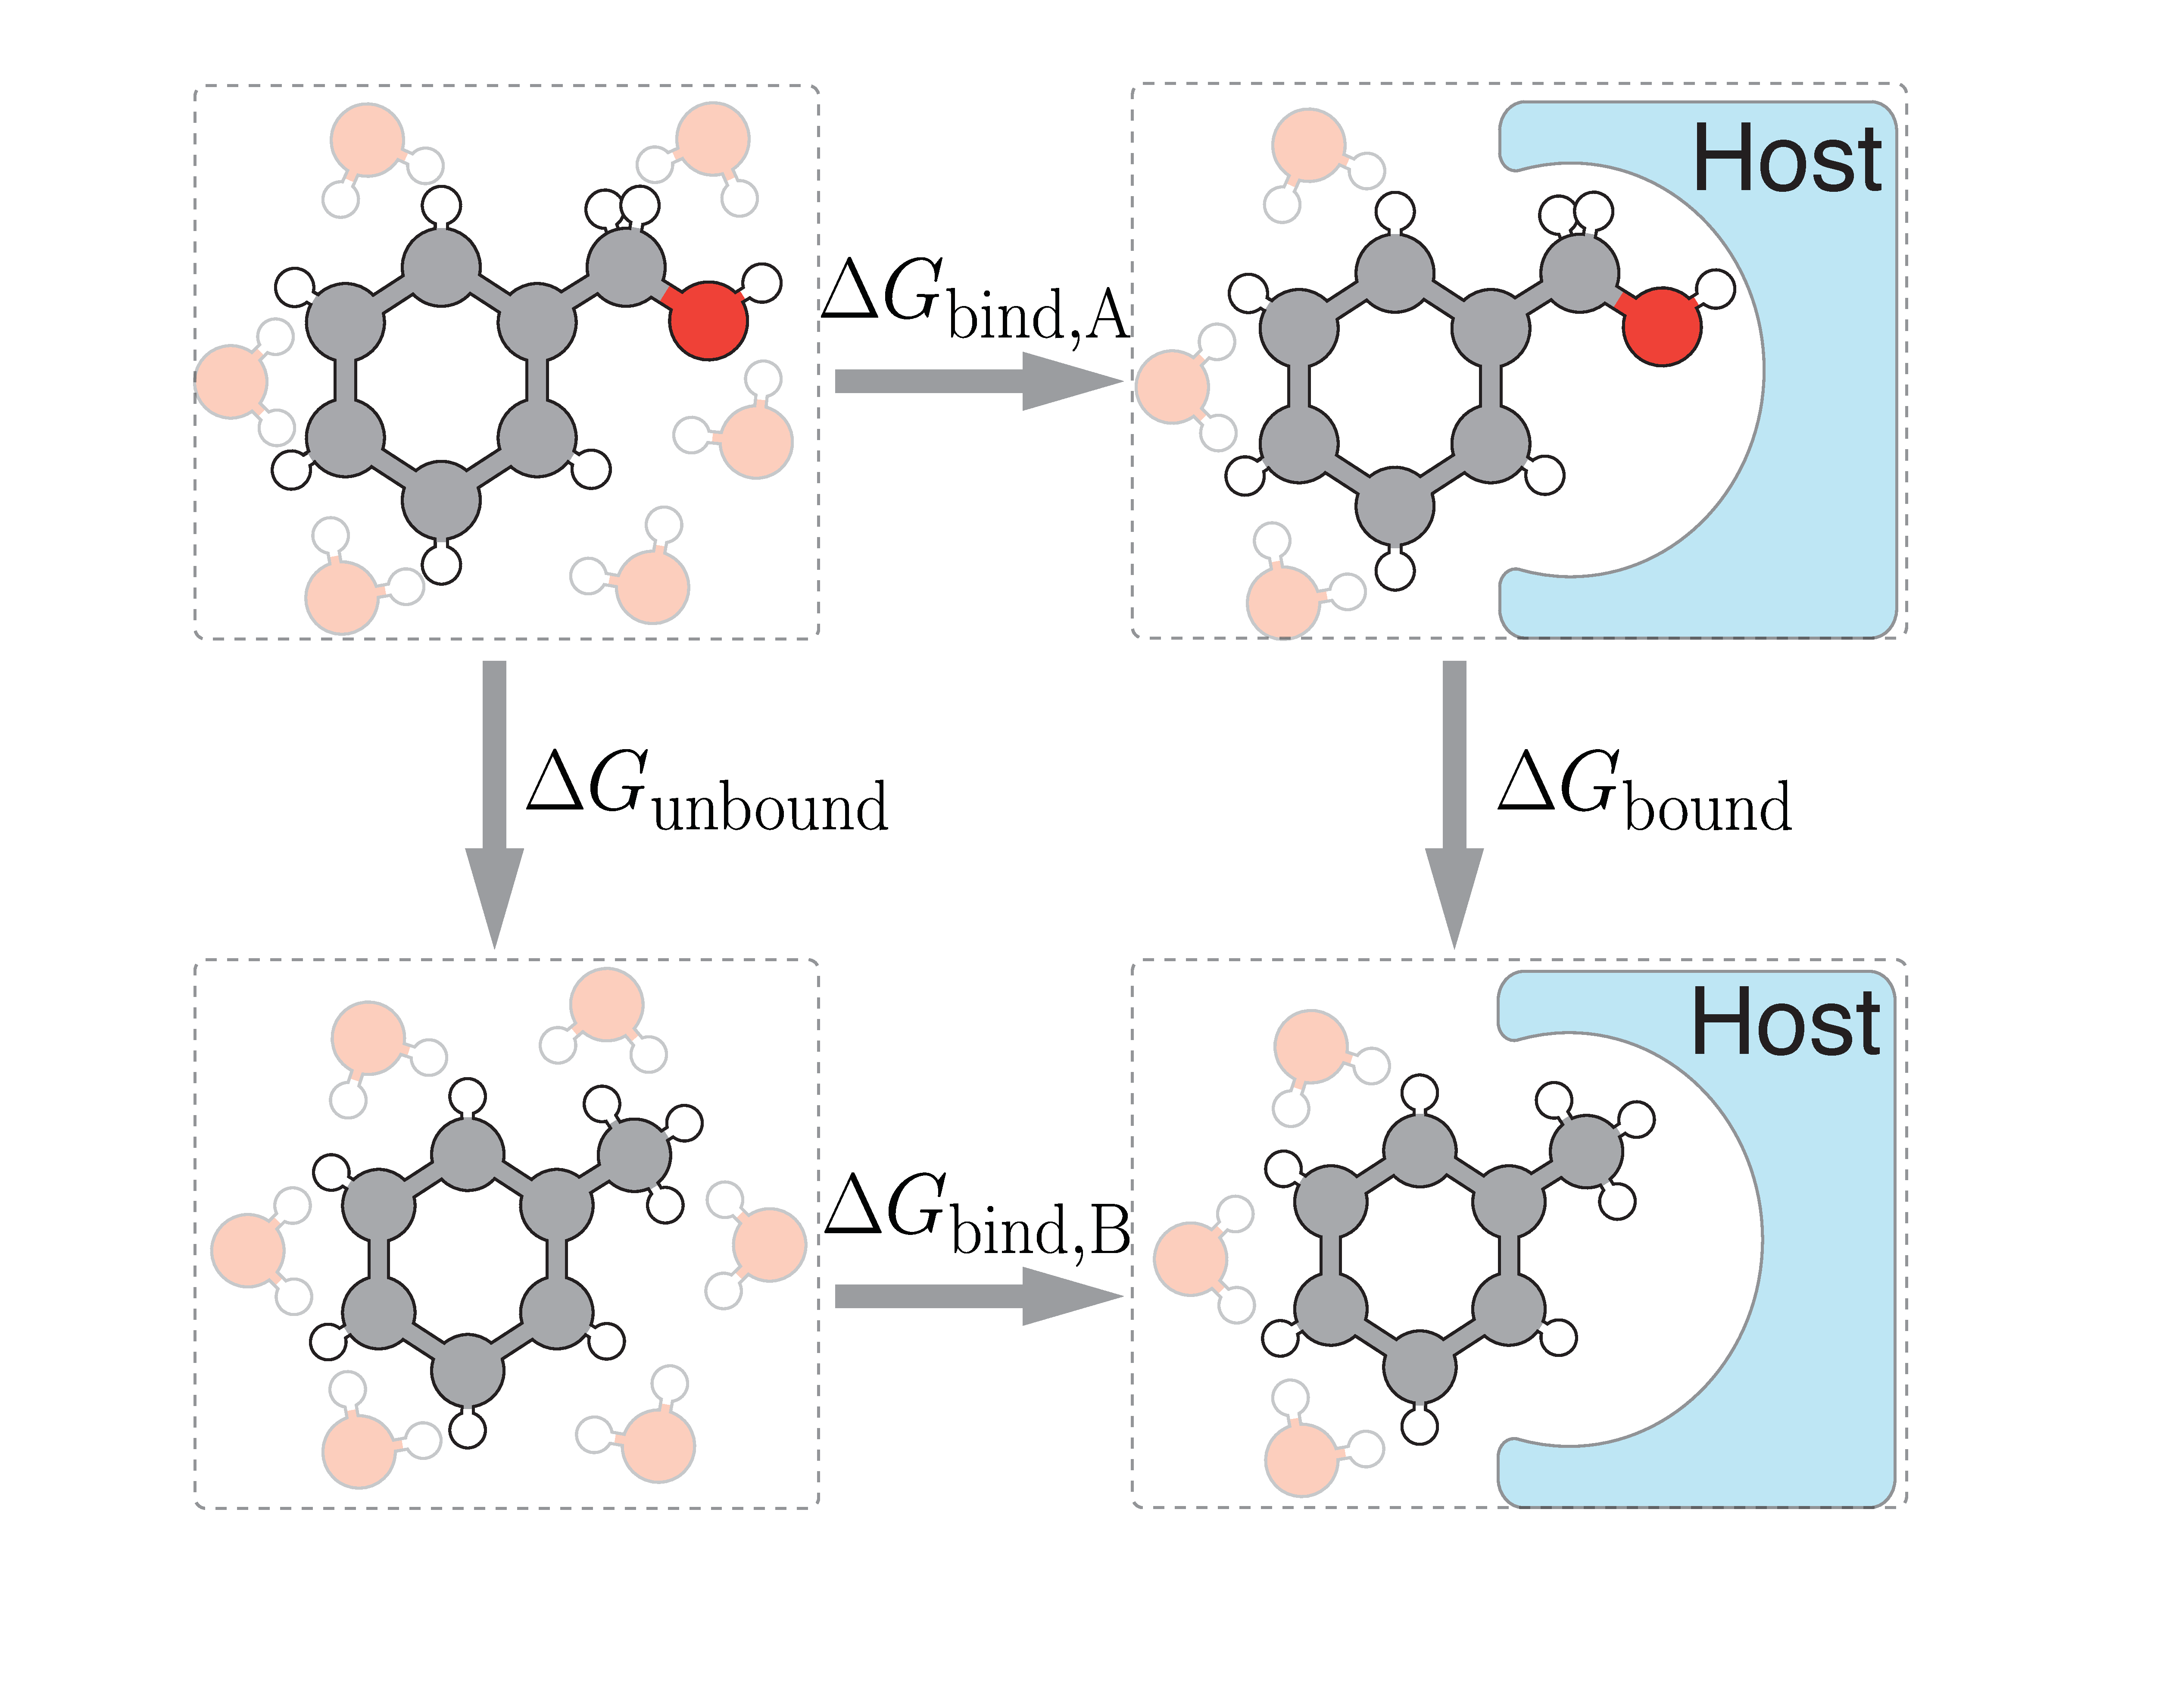
\includegraphics[width=0.95\linewidth]{figures/fig2_therm_cyc/Figure.pdf}
    \caption{{\bf Thermodynamic cycle for computing the relative free energy of binding ($\Delta \Delta G$) between two related small molecules to a supramolecular host or a rigid receptor.}
    The relative binding free energy difference between two small molecules, $\Delta \Delta G_{\mathrm{bind}, A \rightarrow B} \equiv \Delta G_{\mathrm{bind}, B} - \Delta G_{\mathrm{bind}, A}$---here benzyl alcohol (top) to toluene (bottom)---can be computed as a difference between two alchemical transformations, $\Delta G_\mathrm{bound} - \Delta G_\mathrm{solvated}$, where $\Delta G_\mathrm{bound}$ represents the free energy change of transforming $A \rightarrow B$ in complex, i.e. bound to a host molecule, and $\Delta G_\mathrm{unbound}$ the free energy change of transforming $A \rightarrow B$ in solvent, typically water.}
    \label{fig:fig_binding_thermodynamic_cycle}
\end{figure}

\paragraph{How are alchemical transformations performed in practice?}

In practice, the mutation of $A$ to $B$ is carried out by introducing one or more parameters $\vec{\lambda}$ controlling the potential energy function $U(\vec{q};\vec{\lambda})$ such that the potential of compounds $A$ and $B$ is recovered at two particular values $\vec{\lambda}_A$ and $\vec{\lambda}_B$.
Briefly, this is achieved by simulating a ``chimeric'' molecule composed of enough atoms to represent both $A$ and $B$.
A subset of the energetic terms in $U(\vec{q};\vec{\lambda})$ is then modulated by $\vec{\lambda}$ so that at $\vec{\lambda}_A$, the atoms that form molecule $A$ are activated and those belonging exclusively to $B$ are non-interacting ``dummy atoms'', while the opposite occurs at $\vec{\lambda}_B$ (see Sec.~\ref{sec:relative-fe-protocol} for details).

We can rigorously account for fluctuations in other thermodynamic parameters such as changes in volume $V$ when simulating at constant pressure $p$ or changes in number of molecules $N_i$ of species $i$ at constant chemical potential $\mu_i$ (e.g., number of waters or ions) by introducing the \textit{reduced potential}~\cite{shirts2008statisticallya}
\begin{equation}\label{eq:reduced-potential}
u(\vec{q};\vec{\lambda}) \equiv \beta \left[ U(\vec{q};\vec{\lambda}) + p \, V(\vec{q}) + \sum_i \mu_i \, N_i(\vec{q}) + \cdots \right] \, .
\end{equation}
Here, the collection of thermodynamic and alchemical parameters $\{\beta, \vec{\lambda}, p, \mu, \ldots\}$ defines a \emph{thermodynamic state}.
In the context of alchemical calculations, in which the thermodynamic states vary only in their value of $\vec{\lambda}$, these are also referred to as \emph{alchemical states}.
The free energy of mutating $A$ to $B$ in any environment ($\Delta G_{\mathrm{env}}$ e.g., binding site, solvent) can then be computed as
\begin{equation}\label{eq:delta-G-env}
    \Delta G_{\mathrm{env}} = - k_BT \ln \frac{Z(\vec{\lambda}_B)}{Z(\vec{\lambda}_A)} = - k_BT \ln \frac{\int_{\Gamma_{\mathrm{env}}} \exp\left( u(\vec{q}; \vec{\lambda}_B) \right) \, d\vec{q}}{\int_{\Gamma_{\mathrm{env}}} \exp\left( u(\vec{q}; \vec{\lambda}_A) \right) \, d\vec{q}} \, ,
\end{equation}
over the configurational space of the environment ($\Gamma_{\mathrm{env}}$).
While it is generally not feasible to compute the two partition functions $Z(\vec{\lambda})$, several estimators have been devised to robustly estimate the ratio of partition functions in Eq.~\ref{eq:delta-G-env} (see Sec.~\ref{subsec:estimators}) from a set of configurations usually collected with MD simulations from the thermodynamic states defined at $\vec{\lambda}_A$ and $\vec{\lambda}_B$ and intermediates thereof.

\paragraph{Why do alchemical calculations need unphysical intermediate states?}
While it is theoretically possible to estimate the ratio of partition functions from samples collected only at states $\vec{\lambda}_A$ and $\vec{\lambda}_B$, the efficiency of the free energy estimators rapidly decreases as the phase-space overlap between the two states also decreases~\cite{wu2005phasespace, wu2005phasespacea}.
Roughly, the phase-space overlap between two thermodynamic states measures the degree to which high-probability configurations (i.e., those with very negative potential energy) in one state are also high-probability configurations in the other state (see Sec.~\ref{sec:are-they-good} and Fig.~\ref{fig:fig_what_is_lambda}).

Equilibrium free energy calculations, our focus here, solve the problem of having poor overlap between the states of interest by introducing multiple intermediate alchemical states at values $\vec{\lambda}_A = \vec{\lambda}_0, \vec{\lambda}_1, \cdots, \vec{\lambda}_K = \vec{\lambda}_B$ so that each pair of consecutive states $\vec{\lambda}_k, \vec{\lambda}_{k+1}$ share good overlap.
Each intermediate state models a ligand that is neither $A$ nor $B$ but a interpolation of the two.
Many estimators (e.g., exponential reweighting (EXP)~\cite{zwanzig1954hightemperature} and Bennett's acceptance ratio (BAR)~\cite{bennett1976efficient,shirts2003equilibrium}) can then be used to compute the free energy as
\begin{equation}
    \Delta G_{\mathrm{env}} = k_BT \sum_{k=0}^{K-1} \Delta f(\vec{\lambda}_k, \vec{\lambda}_{k+1}),
\end{equation}
from samples collected at all the alchemical states $\{\vec{\lambda}_k \}$, where $\Delta f$ is the \emph{unitless free energy difference}
\begin{equation}
    \Delta f(\vec{\lambda}_k, \vec{\lambda}_{k+1}) = f(\vec{\lambda}_{k+1}) - f(\vec{\lambda}_k) = - \ln \frac{Z(\vec{\lambda}_{k+1})}{Z(\vec{\lambda}_k)} \, .
\end{equation}
While this strategy usually results in sampling thermodynamic states whose Boltzmann distributions are very similar, thus collecting information that is to some degree redundant, some estimators, such as the Multistate Bennett acceptance ratio (MBAR)~\cite{shirts2008statisticallya}, can exploit similarities between states to improve the precision of the estimates. This is achieved by using the configurations sampled at all alchemical states $\{\vec{\lambda}_k \}$ to compute the free energy difference $\Delta f(\vec{\lambda}_i, \vec{\lambda}_{j})$ between any pair of states $i,j$ (see Sec.~\ref{subsec:estimators}).

Non-equilibrium free energy techniques provide an alternate approach to this problem, driving $\lambda$ between states, but these are not our focus here.~\cite{jarzynski1997nonequilibrium,jarzynski1998equilibrium,crooks2000pathensemble, gapsys2020large}

\paragraph{How do absolute free energy calculations differ from relative?}

While absolute and relative free energy calculations have subtle differences in their practical applications (e.g., use of restraints, handling of the standard state), the fundamental ideas and concepts of relative free energy approaches remain unaltered in other types of alchemical calculations.
Absolute binding, hydration, and partition free energies still use thermodynamic cycles that enable computing transfer free energies without actually simulating the physical transfer from one environment to another.

The main difference in these approaches lies instead in the thermodynamic cycle to which this strategy is applied.
For example, a typical thermodynamic cycle for an alchemical absolute binding free energy calculation is represented in Fig.~\ref{fig:fig_absolute_thermodynamic_cycle}.
In this case, two independent calculations compute the free energy of removing the interactions between the ligand and its environment in solvent or in the binding site respectively through a series of intermediate states in which the energy terms are only partially deactivated.




%%%%%%%%%%%%
% Step 0   %
%%%%%%%%%%%%
\section{\tocorange{What can be expected from alchemical simulations?}}
\tocsectioncomment{Steering Meeting: @Volunteer Shorten and move most material to second paper. Possibly add a walkthrough of a ``dummy calculation'' (which could be a particular realisation of a general workflow laid out in @Jenke Scheen's figure)? This could lead on to discussion of particular methods. @Toni Mey I could do this}
\label{sec:step0}
When starting an alchemical free energy project, a key first step is to decide whether free energy calculations are really the right tool. Particularly, count the cost of your
project: Can you even hope to tackle the problem with available resources and, if successful, will it
be worth it in terms of human and computational cost?

\subsection{How accurate are alchemical free energy calculations?}
\label{subsec:expectation}
We first note that the accuracy of any free energy calculation method will depend on the quality of the underlying force field.  Therefore, any description of the force field for the molecules under study must be carefully checked to be sufficiently accurate to experiment. In particular, one must make sure that if using automatically generated molecular descriptions from either one's own workflow or some other computational chemistry program, there are no obvious problems in these files either through errors in the workflow, or lack of chemical coverage in the data used to construct the molecular description. Torsional parameters, in particular can be misassigned or improperly parameterized. 

Alchemical free energy calculations involving small molecules seem to achieve, in favorable cases, root mean square (RMS) errors relative to experiment around 1-2 kcal/mol depending on force field, system, and a variety of other factors such as simulation time, sampling method, and whether the calculations employed are absolute or relative. A small selection of example datasets and case studies can be found in Sec.~\ref{sec:benchmark} at the end of this document.
However, the domain of applicability is a significant concern~\cite{sherborne2016collaborating, cournia2017relative}, especially for relative calculations, which typically require a high quality and usually experimental bound structure of a closely
related ligand as a starting point. Additional factors such as slow protein or ligand rearrangements, uncertainties in ligand binding mode, or charged ligands can make these calculations far less reliable and more of a research effort.


It is worth noting that the accuracy of free energy calculations is highly variable across different protein targets, and likely across different ligand chemotypes as well.
For instance, FEP+ with OPLS3 achieves an RMSE of 0.62 kcal/mol for a set of 21 compounds binding to JNK1 kinase, but an RMSE of 1.05 kcal/mol for a set of 34 compounds binding to P38$\alpha$ kinase~\cite{harder2016opls3}.
Furthermore, perturbations for the same chemotype in different pockets of the BACE enzyme gave varied errors~\cite{keranen2017acylguanidine}. Here the errors refer to the difference in $\Delta G$ derived from calculated $\Delta \Delta G$'s while fitting a constant offset to best reproduce the experimental binding free energies for known compounds~\cite{wang2015accurate}. Each $\Delta \Delta G$ is associated with a particular free energy calculation or transformation, which can be thought of as an edge in the graph spanning the compound series, see examples of such graphs in Fig.~\ref{fig:fig_types_of_networks}.

The fact that we can analyze both $\Delta G$ values and $\Delta \Delta G$ values raises an important question about analysis -- which calculated values should we assess? It is important to be clear on what error to report: $\Delta G$ after shifting by a constant to minimize the RMSE, unshifted $\Delta G$, $\Delta \Delta G$ of computed edges, or $\Delta \Delta G$ of all edges. (See recommendations for reporting best practices, Sec.~\ref{sec:plot_data}.) Additionally, as it is possible to perform calculations on a set of ligands using different pairwise comparisons of molecules, the performance of the method may be biased based on which pairs of comparisons are performed. Additionally, it is possible that the error associated with the relative free energy between a two ligands that was not directly computed,  but can be deduced using one or more thermodynamic paths involving other ligands will likely be more uncertain.
Given the need to understand the performance of the system with alchemical free energy calculations, we recommend that retrospective studies for a particular target and a particular chemical series be performed for each application case.

\subsection{How reproducible are alchemical free energy calculations?}
\label{subsec:reproducible}
We restrict our analysis here to repetitions of the same calculation performed with precisely the same force field, as different force fields used to describe the same molecule can lead to wide differences in free energies in some cases.  Even within this restriction,
finite computing resources necessarily limit the generated number of uncorrelated samples of potential energy surfaces, and therefore alchemical free energy calculations only give free energy estimates to within finite precision. An important consideration is how reproducible alchemical free energy calculations are in practice. In simple cases such as absolute hydration free energies of small organic molecules, or relative hydration free energy calculations between structurally similar small organic molecules, it should be possible to obtain highly precise estimates with a given software package, i.e.with a sample standard deviation under 0.01 kcal/mol~\cite{rizzi2019sampl6}.
For more complex use cases such as protein-ligand binding free energies the repeatability is often substantially worse~\cite{rizzi2019sampl6}. A good practice is to perform two or three runs of the same perturbation to assess precision with a given protocol, using different initial velocities. The sample standard deviation will give a crude estimate of the reliability of the estimates, and whether the precision is sufficient for the problem at hand. When practical, a more stringent test is to use different input coordinates for each repeat run as well as different velocities. 

Note that these types of statistical differences concern calculations carried out with a single software package, but simulation package variations can introduce additional discrepancies. Such issues of reproducibility of free energy calculations across different simulation packages have attracted attention recently~\cite{loeffler2018reproducibility,rizzi2019sampl6}. Greater variability is expected between packages due to methodological differences such as integrators, thermostats, barostats, treatment of long-range electrostatics, and potentially other factors. For absolute and relative hydration free energies of small organic molecules a variability of ca. 0.2 kcal/mol between popular simulation packages has been reported~\cite{loeffler2018reproducibility}. In the recent SAMPL6 SAMPLing challenge a larger variability of 0.3 to 1.0 kcal/mol was noted in the computed absolute binding free energies of host/guest systems even though the study sought to use identical input and simulation parameters~\cite{rizzi2019sampl6} and, in many cases, single-point energies were identical or nearly so. Further work is needed to ensure reproducibility of alchemical free energy calculations across different software implementations to guarantee that force-field development efforts lead to transferable potential energy functions. 

\subsection{Is my problem suitable for alchemical free energy calculations?}
\label{subsec:suitability}
Before even planning free energy calculations to study binding to a
particular target, it is important to assess what is known about the
system and its timescales and its suitability for free energy
calculations, as well as the \emph{purpose} of the calculations and
the amount of available computer resources. In some cases, predicting accurate binding free energies for a particular target might be
\emph{more} challenging than simply measuring them! This is
often the case when dealing with database screening problems, where
compounds might be easily and quickly available commercially for
testing and free energy calculations could consume far more resources. Free energy calculations thus typically only
appeal when (slow or costly) synthesis would be required or experiments are otherwise cost-prohibitive.

Sometimes, however, free energy calculations can provide answers that are not
readily available from experiments. For example, type II kinase
inhibitors selectively bind to different kinases in the so-called
DFG-out conformations~\cite{schindler2000structural}. The selectivity of such
inhibitors may be attributed either to their differential binding to
different kinases in the DFG-out conformations, or to different
stability of the DFG-out conformations of different kinases. 

Let
$K_C$ be the equilibrium constant between DFG-in and DFG-out
conformations of one kinase, and $K_D^\ast$ be the dissociation
constant of a type II inhibitor against this kinase, the apparent
binding constant of this inhibitor against this kinase is then
\begin{equation}
  K_D = K_D^\ast \frac{1 + K_C}{K_C}
  \label{eqn:conformational-binding}
\end{equation}

Since binding experiments cannot resolve $K_D^\ast$ and $K_C$ individually, such experiments cannot address the basis of selectivity of the type II inhibitors. Absolute binding free energy calculations, in contrast, can take advantage of the slow kinetics of DFG-in/out conversion, and estimate the conformation-specific binding constant $K_D^\ast$, thus yielding clues as to the source of selectivity.

%
%%%%%%%%%%%%%%%%%%%%%%%%%%%%%
% Simulation prerequisites  %
%%%%%%%%%%%%%%%%%%%%%%%%%%%%%
%
\section{\tocorange{Simulation prerequisites}}
\tocsectioncomment{There was substantial interest in expanding this section (see initial suggestions/ discussion).}
\tocsectioncomment{@Irfan Alibay/ @Volunteer to suggest additional points.}
\tocsectioncomment{@Irfan Alibay/ @Emilio Gallicchio/ @Volunteer to expand on approaches for explicitly accounting for protonation/ tautomer changes.}
\tocsectioncomment{@Hannah Bruce Macdonald/ @David Slowchower/ @Vytas Gapsys/ @Volunteer to expand range of systems discussed, e.g. membrane proteins, cofactors, multimers, PPIs.}
\label{sec:prerequisites}
Alchemical free energy protocols as discussed below (Sec.~\ref{sec:simulation_protocol_choice}) are defined for a specific type of free energy calculation, i.e. a free energy of binding or a free energy of hydration. Different types of simulations require different choices for ligands, solvent, and host molecules (in the case of the estimation of free energies of binding).

\subsection{Free energies of binding}
\tocsubsectioncomment{{Steering Meeting: @Volunteer move paragraph ``Congeneric series often need alignment'' to second paper if we are assuming a single calculation?}}
\label{subsec:binding}
In principle, in the limit of sufficient configurational sampling, the free energy changes estimated from an alchemical free energy calculation should be independent of the system's initial coordinates. However, in practice, because simulations are of finite duration (typically 1-100 ns per state at present), this is only true for certain classes of alchemical free energy calculations such as relative or absolute free energies of hydration of small and relatively rigid organic molecules. Protein-ligand complexes typically exhibit slowly relaxing degrees of freedom that significantly exceed the duration of an alchemical free energy calculation, and host-guest calculations can be susceptible to these issues as well, depending on timescale and system. It is therefore generally important to carefully select input coordinates to obtain satisfactory results. 
The following questions may be relevant before diving into the simulation setup.

\begin{itemize}
    \item Do I have one or multiple good receptor structures? (e.g. a good resolution X-ray crystal of the protein target)
    \item Do I have information on one or all of the ligand binding sites? (e.g. an X-ray structure)
    \item Should I include buried waters, or other small molecules that can be found in an X-ray structure?
    \item Are my ligands part of a congeneric series? (i.e. simple R group substitutions around the same scaffold)
    \end{itemize}

\paragraph{Are there good X-ray structures available?}
As with any simulation, care should be taken in selecting available X-ray structures in the Protein DataBank~\cite{berman2003announcing}. In some cases it may be wise to choose multiple starting structures to account for variability in receptor conformations as well as the accuracy of available X-ray structures. Typically, clustering of receptor structures can be used to identify different receptor conformations near the binding site, as well as assessing relevant side chain placements from the X-ray structure, see for example~\cite{mey2016blinded}. In terms of set up and other choices, following general best practice guidelines is advisable~\cite{braun2019best}.

Many free energy calculations focus on a congeneric series of ligands, which can make these calculations suitable for relative free energy protocols (see Sec.~\ref{sec:simulation_protocol_choice}). For relative calculations, some care has to be taken selecting binding poses for these ligands. Generally, a common assumption for a congeneric series is that the binding mode is conserved. Therefore, if an X-ray structure of one of the ligands is available, this should be used to position the ligands in the putative binding site in an energetically reasonable conformation without steric or electrostatic mismatch with the receptor. Checking the X-ray structure versus the experimental electron densities is important, as the position of part of the ligand or important sidechains may be based on the interpretation of the crystallographer rather than the available electron density, especially in cases of missing density. For example, looking at a cyclohexane ring density, a chair configuration is vastly more likely than that of a boat and, if a boat configuration is present in the structure, it may be worth inspecting the density to ensure it adequately supports this choice. 

\paragraph{Are you prepared to deal with any binding mode challenges?}
Generally, binding modes within congeneric series are conserved~\cite{wacker2010conserved}, however, exceptions exist~\cite{brandt2011congeneric,nazare2005probing}, as discussed in more detail in Sec.~\ref{sec:multiple_binding_modes}. Certain functional groups may be particularly prone to this due to symmetries or near symmetries. One such issue involves a 180 degree flip in the dihedral angle of an aromatic ring, or five-membered ring leading to a different spatial position of ortho- or meta- substituents that otherwise should overlap within a series. The 180 degree flip of the ring may not occur enough during simulations (due to steric obstructions) to overcome bias due to the starting configuration. Another scenario may be equatorial and axially substituted saturated rings (e.g. cyclohexane derivatives). This situation may be addressed by explicitly modelling different binding modes of the same ligand and combining later computed free energy differences for different binding modes into a relative free energies of binding~\cite{kaus2015how}.

\paragraph{Have you considered stereoisomers and enantiomers?}
Congeneric series can contain stereoisomers or enantiomers which can bind very differently, resulting in large errors if treated incorrectly. For racemates, the relative abundance of each stereoisomer is normally not known. Therefore, the experimental activity associated with just one stereoisomer/enantiomer is more uncertain. However, the modeling typically uses just the bioactive conformation that best fits the active site. Clearly this introduces potential for larger errors compared to experiment. Nevertheless, if all compounds in the congeneric series are racemic, originating from similar synthetic procedures with an expected similar abundance of stereoisomers, then the differences may cancel and the trend in calculated and observed binding energies may be robust. Despite this, we can see that care and further testing is needed in this scenario, and the quality of the predictions may suffer. Additionally, unexpected changes in what stereoisomer binds experimentally, if they occur, could pose significant challenges for modelling efforts.

\paragraph{Conserved binding site waters can play an important role in binding free energies}
Binding site water molecules may form water mediated protein-ligand interactions which can pose challenges whenever exchange with bulk water is slow compared to simulation timescales. This happens typically in buried binding sites. Overlaying multiple protein X-ray structures can identify conserved or additional water molecules that can be useful to include in calculations. In cases where water molecules are known to play an important role in the binding, software implementations that use water sampling facilitated by Grand Canonical Monte Carlo methods may be useful~\cite{michel2010prediction}. Other tools such as WaterMap or open source equivalents (SSTMap, GIST, and others) can be used to define water structure for systems with no experimental evidence of water sites~\cite{wang2011ligand}. Well-known protein systems with water mediated ligand interactions are for example: HSP90 which formed part of the D3R grand challenge 2015~\cite{mey2016blinded}, A2A~\cite{brucemacdonald2018ligand}, MUP~\cite{ross2015water}, ~\cite{deflorian2020accurate}, and others~\cite{michel2009energetics}.

\paragraph{Protonation states depend on the pH of the experimental assay}
Care should be taken when preparing ligands and proteins to match the pH of the experimental assay, if known. As mentioned above in Sec.~\ref{subsec:exp_condition}, the pH of the assay can differ from neutral pH and will determine the protonation states of the proteins and ligands. Since the pKa of reference amino acid sidechain residues is known, but can vary in the protein environment, many different tools have emerged for predicting sidechain pKa in proteins, such as the H++ server, ProPKa, APBS, and Maestro ~\cite{anandakrishnan2012automating, sondergaard2011improved, jurrus2018improvements, 2020schrodinger}. Strongly acidic (Glu, Asp) or basic (Arg, Lys) sidechains can reliably be predicted to be ionized, but care is still needed as the local environment can modify expected ionization states, such as  the catalytic Asp dyad in proteases. Histidine is notoriously more difficult to predict as its pKa suggests it ionizes closer to the experimental pH range. For ligands, often the pKa needs to be determined, if it is not known experimentally. There are many different available tools for this purpose, but common choices may be propKa~\cite{olsson2011propka3,sondergaard2011improved}, Chemicalize (\url{https://chemicalize.com/welcome}), or Maestro~\cite{2020schrodinger}. Still, accurate pKa prediction for small molecules remains a challenging problem, even with dedicated tools~\cite{isik2018pka}. While often it can be assumed that the protonation state of a ligand and protein will remain the same as the ligand binds, some care needs to be taken with systems where the protonation state may change upon binding~\cite{onufriev2013protonation}. BACE~\cite{kim2015conformational}, for example, famously undergoes a protonation state change on ligand binding.


\paragraph{Congeneric series often need alignment}
Input coordinates for a congeneric series may be generated by docking calculations, or by ligand alignment using MCSS algorithms. The latter tends to produce alignments that are more conserved and more consistent free energy changes across a dataset, but will struggle to yield reasonable results for relative binding free energy calculations that involve a significant binding mode rearrangement. This may also lead to steric clashes with the receptor coordinates of the reference ligand if structural rearrangements are needed to accommodate different members of the congeneric series. Small steric clashes may be resolved during subsequent simulation equilibration prior to data collection, but there is a risk that the complex relaxes to an alternative metastable state. 

An additional consideration arises for single topology relative free energy calculations. In this class of alchemical free energy calculations it is necessary to generate a molecular topology that may describe the initial and final states of the perturbation (see Fig.~\ref{fig:fig_topology}). In cases where the end states have high topological similarity and high structural overlap this is relatively straightforward and typically handled by use of MCSS calculations. In situations where the end state topologies differ significantly, or where there is relatively little spatial overlap between the two end states, some user intervention may be necessary to produce a satisfactory input topology.

If the binding site location is uncertain but the structure of the receptor is well defined and plausible binding sites are identified, it may be more useful to choose an absolute free energy protocol to compute the standard free energy of binding of the ligand to a set of binding sites. This requires the user to prepare input files describing the bound conformation in different putative binding sites~\cite{evoli2016multiple}. The apparent binding free energy of the ligand may be obtained by combining the individual binding site free energies, which also indicate where the ligand is more likely to bind. In this case a docking program can generate initial structures. Different commercial and non-commercial tools are available, such as rDock~\cite{ruiz-carmona2014rdock}, Autodock Vina~\cite{trott2010autodock}, Glide~\cite{friesner2004glide}, or Flare, to name a few~\cite{kuhn2020assessment}. 

If the putative binding sites are not apparent, for instance due to significant induced-fit effects, it may be challenging to obtain meaningful free energies of binding. One may have to account for the free energy cost of forming a binding site in the target receptor which may not be feasible on alchemical simulation timescales.

\subsection{Free energies of hydration or partition coefficients}
\tocsubsectioncomment{Steering Meeting: @Volunteer to expand coverage of free energies of hydration/ partition coefficients to make coverage of applications more equal.}
\label{subsec:hydration}
Preliminary considerations necessary for using free energy methods to compute partition coefficients are generally more straight forward. For example, a 3D minimised structure of a solute can be generated with a simple tool such as openBabel and solvated to prepare the input to compute a free energy of hydration~\cite{oboyle2011open}. However, in these cases a careful choice of forcefield for the organic solvent model, as well as water model is essential. See for example~\cite{bosisio2016blinded,rustenburg2016measuring} for a good discussion of these choices. And, while sampling problems might seem to be a non-issue for small molecules, this is not always the case; e.g. even the hydroxyl orientation on neutral carboxylic acids can occasionally pose a challenge~\cite{klimovich2010predicting, lim2019assessing}.

%%%%%%%%%%%%%%%%%%%%%%%%%%%%%%%%%%%%%%%%%%%%%%
% What simulation protocol should I choose   %
%%%%%%%%%%%%%%%%%%%%%%%%%%%%%%%%%%%%%%%%%%%%%%
\section{\tocorange{What simulation protocol should I choose?}}
\tocsectioncomment{Steering group: Possibly expand to include other methods group agrees on.}
\tocsectioncomment{@Stefan Boresch to restructure as per his suggestion to remove single/dual topology section and begin with a more fundamental discussion which might more naturally include all options e.g. ATM. @Stefan Boresch to mention best practices for dummy atoms? This might benefit from following @Emilio Gallicchio's changes to make the theory section more general.}
\tocsectioncomment{@Sheenam Khuttan / @Emilio Gallicchio to contribute section on ATM.}
\tocsectioncomment{@Vytas Gapsys / @Volunteer to add best practices for non-equilibrium calculations.}
\label{sec:simulation_protocol_choice}
Alchemical free energy calculations can be grouped into two main categories, ``absolute'' (see Fig.~\ref{fig:fig_absolute_thermodynamic_cycle}) and ``relative''\footnote{The distinction is a bit of a misnomer, since both compute ratios of partition functions relative to another state and in that sense are relative, while neither computes an absolute free energy.} (see Fig.~\ref{fig:fig_binding_thermodynamic_cycle}), which differ in whether they compute properties for a single molecule (absolute) or compare properties of different, usually closely related, molecules (relative).
To use binding as a concrete example, in absolute binding free energy calculations, we compute the binding free energy of a ligand to an individual receptor relative to a standard reference concentration. In contrast, in relative binding free energy calculations, we compare the binding free energy of two related ligands to determine the potency difference.

\subsection{Absolute and relative free energy calculations have important differences}
Many of the issues around simulation setup and protocol choice for alchemical calculations are common, but there are some differences between absolute and relative calculations. We will consider protocol differences before treating the common elements.

\subsubsection{Choices unique to relative free energy calculations}
\tocsubsubsectioncomment{Steering Group: @Volunteer to mainly move atom mapping section to second paper and assume that the change is small (and hence atom mapping is trivial). @Benjamin Ries to add discussion of 3D atom mapping in second paper.}
\label{sec:relative-fe-protocol}

\paragraph{Topologies} 
A critical first step is to determine which approach to use for atom mapping between end state molecules. Often this is predetermined by the choice of simulation software. Typically it is possible to chose between a \emph{dual topology} versus a \emph{single topology}

The distinction between single and dual topology can be illustrated by considering a hypothetical transformation from molecule A to molecule B, where both atoms share a common substructure but differ in their substituents; in particular, consider a transformation of benzene to benzyl alcohol shown in Fig.~\ref{fig:fig_topology}.
In this case the common substructure between the two molecules is the benzene ring, though in practice substructure may be selected to be larger depending the mapping chosen, as we discuss below.

In single topology calculations, the overall transformation is set up to involve as few additional atoms as possible, so benzene would be typically changed into benzyl alcohol by first changing one of the hydrogens into a carbon. The site of this transformation will also be the future home of two additional hydrogen atoms bound to the new carbon, so these must initially be present as non-interacting atoms called ``dummy atoms'', which retain their bonded interactions but do not interact with the rest of the system.  Bond parameters as well as partial charges between the changing atoms are adjusted accordingly between the initial and final state. 
Thus, in a single topology calculation, atoms may change their type, ensuring minimal dummy atoms are created. This is illustrated in the left arm of Fig.~\ref{fig:fig_topology}. 

In contrast, in a dual topology alchemical free energy calculation, \emph{no atoms are allowed to change type}~\cite{boresch1999role, shirts2012best}. This means that the benzene to benzyl alcohol transformation involves starting with benzene plus the non-interacting dummy atoms making up the hydroxymethyl group, then passing through an intermediate state where some atoms are partially interacting---particularly, those atoms which are becoming dummy atoms or ceasing to be dummy atoms~\cite{mobley2014blind}. The transformation finally culminates in a state where benzyl alcohol is present along with the additional dummy atom which was previously a corresponding hydrogen of the benzene. Fig.~\ref{fig:fig_topology}'s right branch depicts how such a dual topology works. 

\begin{figure}
    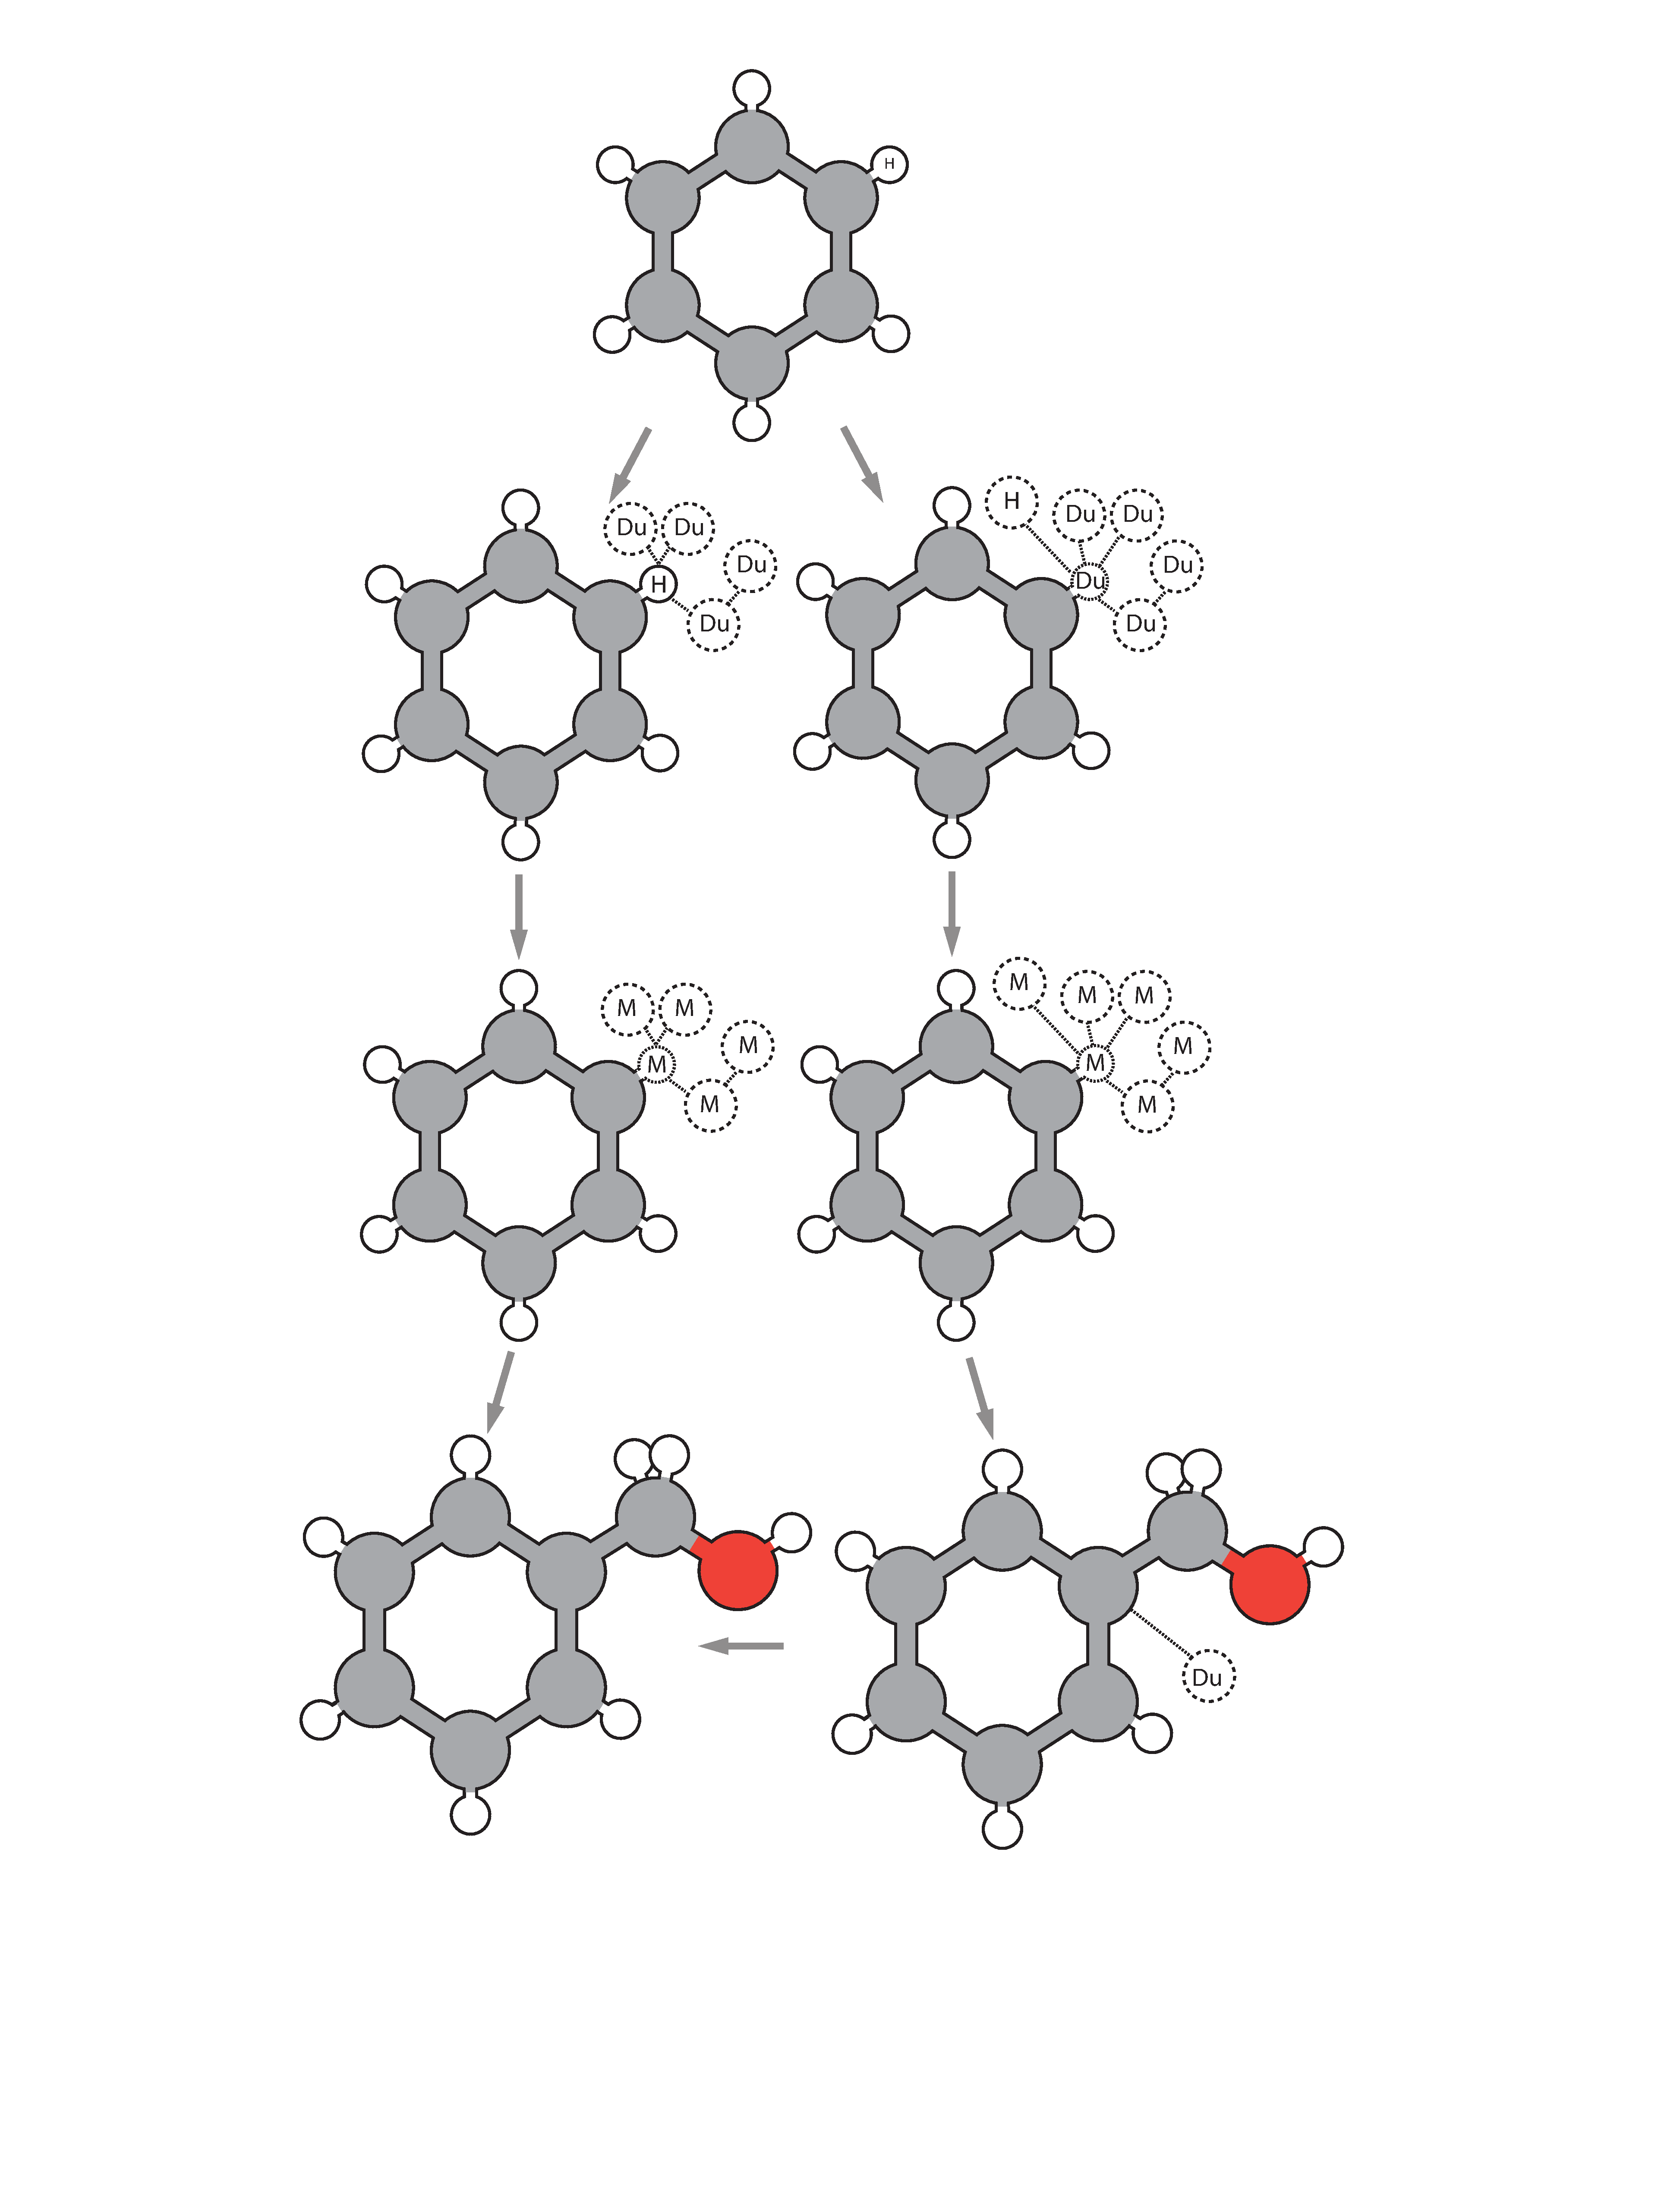
\includegraphics[width=0.95\columnwidth]{figures/fig3_topol/Figure.pdf}
    \caption{\textbf{Two common topologies for alchemical calculations: single and dual topology.} \textbf{Left}: A single topology converts from one type of atom to an other. Dummy atoms (Du) are used when there is no corresponding maximum common substructure match between the two molecules for certain atoms, using a soft-core interaction to improve overlap between the dummy atoms and the "real" atoms.  \textbf{Right}: The dual topology does not convert one species to another, but only converts between Du atoms and an interacting species, but usually uses soft-core potentials for this. The 'mixed' intermediate atoms (M) are used in both dual and single topology approaches. Only the way the transformation occurs and the end states differ. Following the arrow along the left and right illustrate the differences. Figure adapted from \url{http://www.alchemistry.org/wiki/Constructing_a_Pathway_of_Intermediate_States}}
    \label{fig:fig_topology}
\end{figure} 

As far as we are aware, the distinction between single and dual topology approaches is made primarily for two main reasons. First, this choice affects the alchemical pathway followed, and thus may affect convergence properties---though we are not yet aware of a study of the relative efficiency and merits of these two approaches. Additionally, historically, some simulation packages implemented only one approach and not the other, meaning that the distinction was functional. 

Some additional terms have also been employed to talk about these different intermediate pathways . Particularly, some studies refer to a ``hybrid'' topology approach to free energy calculations~\cite{gapsys2015pmx, gapsys2016accurate, gapsys2020large}, though this term may not yet have achieved widespread use. In this case, "hybrid" seems to indicate that the set up of these free energy calculations involves a hybrid of the two molecules, and much of what is done in these studies uses a single topology approach~\cite{gapsys2020large}.

One final approach, so far in its infancy, has been called ``separated topologies'' and essentially consist of two absolute free energy calculations in opposite directions at the same time, turning one molecule's interactions with the environment off, while turning the other molecule's interaction on~\cite{jiang2019computing, rocklin2013separated}.

Software packages vary in their use of single or dual topology approaches; for example, AMBER TI uses a dual topology approach, while BioSimSpace uses a single topology approach. Please make sure to check what approach is used with your software package of choice, or whether it supports your choice of approach (GROMACS and GROMOS, for example, support both). 
To our knowledge, efficiency differences have not been thoroughly explored, though conventional wisdom suggests that fewer dummy atoms are better, as introducing or removing atomic sites is usually more difficult, requiring more intermediate steps ~\cite{liu2013lead, mobley2012perspective}.

\paragraph{Atom mapping}
Once a particular approach to the topology is selected, a crucial next step is to identify the common atoms which will not be perturbed.
Rigorously, this process typically comprises a MCSS search of the molecules involved to identify the common substructure---though the parameters of the MCSS search will differ depending on whether single or dual topology calculations are planned.
Specifically, with a single topology approach in mind, atom types are allowed to change, so a permissive MCSS search can be done, whereas with dual topology a more strict search is required.
\begin{figure}
    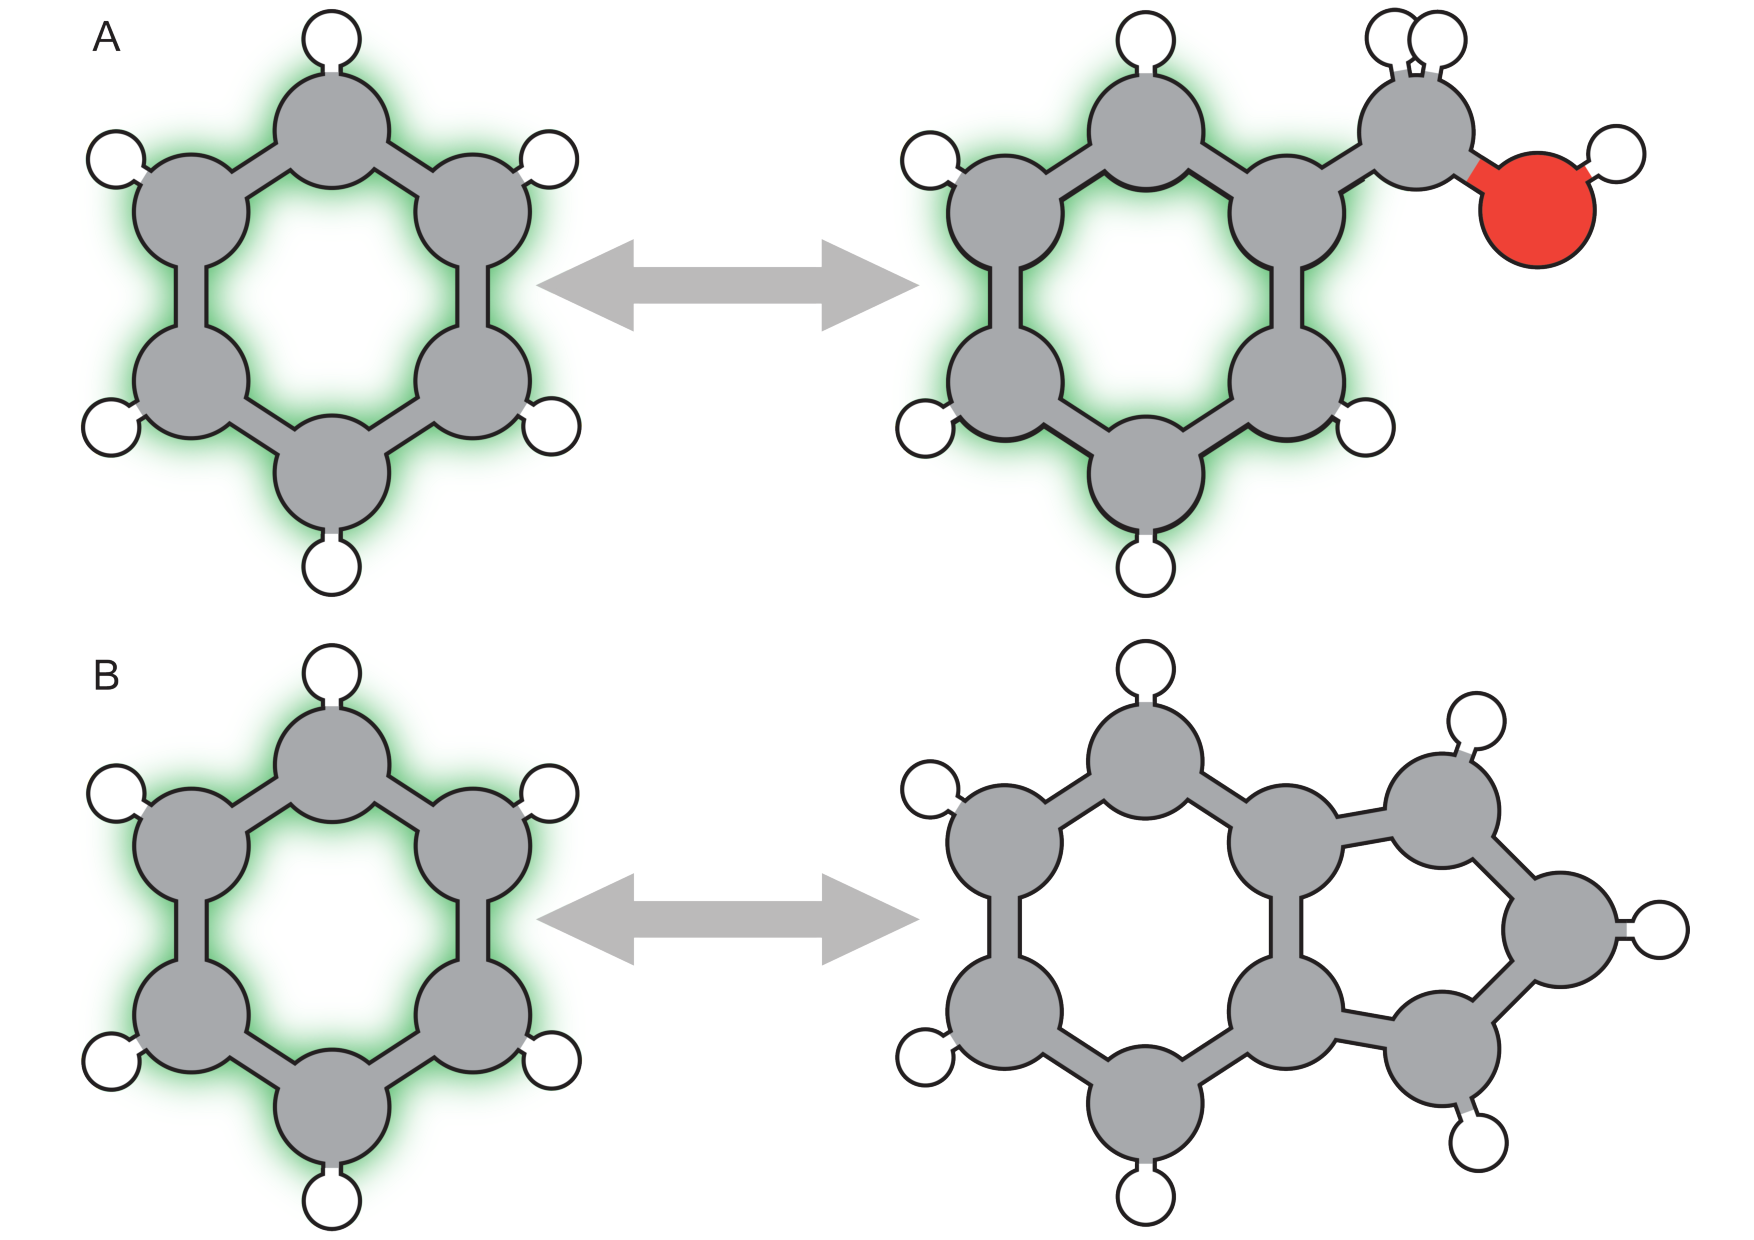
\includegraphics[width=0.95\linewidth]{figures/fig4_mcs/Figure.pdf}
    \caption{\textbf{Illustration of maximum common substructure matches} MCSS is shown in green for when (\textbf{A}) a restrictive MCSS match is used and in (\textbf{B}) ring breaking is allowed, meaning there is no MCSS match between the two compounds.}
    \label{fig:fig_mcss}
\end{figure} 

There are different tools that allow the generation of MCSS matches as well as single topology input. A large number of software tools can compute MCSS matches using different cheminformatics packages. Some rely on RDKit~\cite{rdkit2019Dec}, such as pmx~\cite{gapsys2015pmx}, LOMAP~\cite{liu2013lead}, FESetup~\cite{loeffler2015fesetup} and partially BioSimSpace~\cite{hedges2019biosimspace}, while others such as fkckombu~\cite{kawabata20143d} are standalone tools. Schr\"{o}dinger's FEP+ planning tool was originally based on a version of LOMAP, and it also uses MCSS matching as well as 3D considerations to plan the network of single topology calculations between molecules~\cite{wang2015accurate}. 

MCSS searches can be relatively time consuming, so if the goal is to assess a library of ligands to identify promising pairs for relative calculations, it can be helpful to use faster approaches such as shape similarity to perform an initial similarity assessment and then use MCSS only to identify final mappings for relative calculations~\cite{raymond2002maximum,klabunde2012mars,jones2009elucidating}. The MCSS approach, though relatively standard, takes into account only topological similarity. It is possible that changes in binding mode could actually require a different choice of mapping, so in some cases mappings may need to be planned differently depending on 3D positioning of atoms in space. Visual inspection prior to simulation is recommended to ensure that the mapping criteria correspond to the expected binding mode. If the mapping protocol returns simulations that correspond to different binding modes of a ligand within a perturbation map, this can cause large hysteresis.

Single topology relative calculations and calculations based on substructure searches only work if in fact the ligands share a common substructure, e.g. are part of a congeneric series, see Fig.~\ref{fig:fig_mcss}.
If no common substructure is shared, then alternative dual or separated topology free energy calculations are needed. One would co-localize a pair of compounds in a binding site, exclude their interactions with one another, and compute the relative binding free energy by turning one molecule on from being dummy atoms while turning the other off.
To our knowledge no general pipeline for such calculations yet exists and this would likely remain a research problem. Using an absolute free energy approach instead seems more promising in such a case. 

\paragraph{Ring breaking and forming.} Relative free energy calculations for ring breaking and forming are particularly challenging/problematic (see Fig.~\ref{fig:fig_mcss}\textbf{B}), in part because relative calculations rely on the free energy contributions of dummy atoms canceling between different legs of the thermodynamic cycle, which may not be true whenever dummy atoms are involved in rings~\cite{liu2015ring}.
Some approaches have attempted to address this~\cite{clark2019relative} but a general solution is not yet in mainstream use. Still, FEP+ implements one solution.

\paragraph{Constraints and relative free energy calculations}
One issue which requires particular care is the use of constraints.
Commonly, bonds involving hydrogen are constrained to a fixed length using algorithms such as SHAKE or LINCS, allowing the use of longer timesteps~\cite{krautler2001fast}.
However, in single topology relative free energy calculations, the atoms involved might be mutated to other atom types---for example, in a mutation of methane to methanol, one hydrogen might become an oxygen atom. The bonds with such atoms might not have any constraints, or if all bond are constrained, would have constraints of different lengths. 
Some molecular dynamics engines are not set up to recognize this change, or at least not to correctly include contributions to the free energy from changing constraints/constraint length, so results for a transformation can be erroneous.
At present the most general solution to this problem is simply to avoid the use of constraints (and thus use a smaller timestep if necessary, usually of around 1 fs) in any relative free energy calculation involving a transformation of a constrained bond. Individual software programs and settings can handle such issues. For example, bonds can be transformed in both GROMACS and GROMOS, because contributions of LINCS (GROMACS) and SHAKE (GROMOS) constrained bonds are added to the $\frac{dH}{d\lambda}$ term~\cite{pearlman1993determining, straatsma1992holonomic, pearlman1991overlooked, gunsteren1989computer}. However, the constraints are not taken into account when calculating energy differences to other intermediate states as the effect is entropic, not energetic. User manuals should carefully checked for how these effects are included if a constrained bond changes in length. We do note that if one performs calculations of the changing constraint in both solution and in the binding site, then the errors often cancel substantially, but the cancellation is not guaranteed.

\subsubsection{Absolute free energy calculations must handle the standard state and use restraints}
\tocsubsubsectioncomment{@Emilio Gallicchio to comment on possible issues with theoretical discussion and possibly update in the context of revised theory section. See PR from @Finlay Clark to improve discussion of restraint schemes and automated restraint selection. @Stefan Boresch may like to weigh in on analytical corrections/ general discussion. @Andrea Rizzi to reivew?}
\label{sec:standardstate-restraints}

\begin{figure}
    \includegraphics[width=0.95\linewidth]{figures/fig5_thermo_cyc_abs/Figure_1.pdf}
    \caption{\textbf{Thermodynamic cycle required for an absolute free energy calculation -- absolute free energy of binding example} The fully interacting ligand in water (\textbf{A}), has its charges turned off to pass to (\textbf{B}) followed by turning of van der Waals terms, resulting in a non-interacting ligand in water in (\textbf{C}). Restraints are used on the fully interacting ligand in the binding site of a protein or host molecule (\textbf{D}). The next step is to turn off the charges again (\textbf{E}) followed by the van der Waals interactions resulting in a non-interacting complex state (\textbf{F}). Free energyes can be computed as $\Delta G_{bind} = (\Delta G^{\mathrm{elec}}_{\mathrm{solv}}+ \Delta G^{\mathrm{VdW}}_{\mathrm{solv}})-(\Delta G^{\mathrm{elec}}_{\mathrm{bound}}+ \Delta G^{\mathrm{VdW}}_{\mathrm{bound}}$).
    }
    \label{fig:fig_absolute_thermodynamic_cycle}
\end{figure}

Absolute free energy calculations involve completely removing the interactions between the ligand or solute and its environment, taking it to a non-interacting state that may or may not retain intramolecular non-bonded interactions.
This non-interacting state can then be shifted between environments---from the protein to water, or from one solution to another---without changing its free energy other than that due to the changing volume of the simulations, and then interactions can be restored in the new environment.

Absolute free energies are by definition reported with respect to a specific reference or standard state, which effectively determines the arbitrary point at which the free energy is 0.
The role of the standard state is particularly evident from the expression of the binding free energy between a receptor $R$ and ligand $L$
\begin{equation} \label{eq:DGfromKAB}
    \Delta G = -k_BT ~ \ln \left( c^{\circ} K_b \right)  = -k_BT ~ \ln\left( c^{\circ} \frac{[RL]}{[L][R]} \right) \, .
\end{equation}
Here, the reference state concentration $c^{\circ}$ converts the binding constant $K_b$ into a dimensionless quantity expressed in reference concentration units.
It should be noted that ignoring the term $c^{\circ}$ is equivalent to assuming a reference concentration of 1~D$^{-1}$, where D are the units used to express $K_b$, and would thus cause the value of $\Delta G$ to vary with the choice of the units.
It is convenient to define a standard state at a constant pressure of 1~atm and where each chemical species (i.e., R, L, and RL) in the reaction solvent has a concentration of $c^{\circ}$~=~1~M~=~1~molecule/1660~\r{A}$^3$ but do not interact with other molecules of $R$, $L$, or $RL$.

\paragraph{Handling the standard state in absolute free energy calculations.}
For solvation free energy calculations, handling the standard state is typically straightforward, and treating it correctly simply means ensuring that the non-interacting solute still occupies essentially the same volume as the solute in the interacting system.
So typically in such cases no special care is required to ensure the correct standard state, as long as the \emph{experimental} data being analyzed uses the same standard state.
If this is not the case, a simple entropic correction to the free energy of $k_B T\ln (V_f/V_i) = k_B T \ln (C_i/C_f)$ to the experimental data is needed.

For binding, however, the situation is more complex and requires special care.
Because the simulations are typically performed using restraints and at concentrations that are different from 1 M, the expression of the free energy requires the following correction~\cite{gilson1997statisticalthermodynamic} (see an example of such a thermodynamic cycle in Fig.~\ref{fig:fig_absolute_thermodynamic_cycle})
\begin{equation}\label{eq:restraint-correction}
    \Delta G^{\circ}_{\mathrm{restr}} = -k_BT ~ \ln \left( c^{\circ}{V_L} \right) -k_BT ~ \ln \left( \frac{\xi_L}{8 \pi^2} \right),
\end{equation}
where $V_L$ and $\xi_L$ are respectively the volume of the translational and rotational degrees of freedom of the non-interacting ligand in the simulation box.
When no restraints are used, the non-interacting ligand is free to translate and rotate in the simulation box (i.e., $V_L = V_{\mathrm{box}}$ and $\xi_L = 8\pi^2$), and the rotational term is zero.
A sufficiently thorough exploration of the simulation box by the non-interacting ligand is, however, required for the formula to be valid.
This is typically hard to achieve as the exploration process is governed by diffusion, and weak transient nonspecific binding will occur at other sites on the protein. 
The addition of a restraint limits the volume available to the non-interacting ligand, thus speeding the convergence of the sampling.
In addition, when enhanced sampling methods such as Hamiltonian $\lambda$ exchange are used (see Sec.~\ref{sec:sampling_schemes}), the use of a restraint is typically necessary as it keeps the ligand in the binding site in the interacting state (see also Sec.~\ref{sec:weak-binders}) and generally reduce the round-trip time of replicas.
When restraints are employed, the values of $V_L$ and $\xi_L$ are restraint-dependent, but for commonly employed restraints, these can be usually easily computed analytically or numerically by solving the relevant integral.

\paragraph{Several choices of restraints are possible.}
In practice, a variety of types of restraints are common, from simple harmonic distance restraints between the ligand and the protein~\cite{mobley2006use}, to flat-bottom restraints which work similarly but only exert a force if the ligand leaves a specific region~\cite{chen2007can}.
Because these restraints do not limit the rotational degrees of freedom of the ligand, the rotational term entering the correction in Eq.~\ref{eq:restraint-correction} is zero.

Alternatively, a set of restraints proposed by Boresch have also commonly been employed, where all six rigid-body degrees of freedom governing the orientation of the ligand relative to the receptor are restrained~\cite{boresch2003absolute, leitgeb2005alchemical}.
Further restraints, such as on the overall ligand RMSD have also been used~\cite{woo2005calculation}.

In principle, all of these forms will yield correct binding free energies in the limit of adequate sampling if their effects and connection to the standard state are correctly handled, but they have different strengths and weaknesses.
For example, with more involved restraints, sampling at intermediate $\vec{\lambda}$ values will usually not need to be as extensive but more computational effort must go to computing the free energy to turn on the restraints.
Additionally, such restraints would typically keep the ligand from exploring alternative binding modes. This  restriction may be undesirable when using Hamiltonian $\lambda$ exchange or expanded ensemble techniques where allowing the ligand to exchange binding modes when it is non-interacting could provide sampling benefits~\cite{wang2013identifying}.
More specifically, flat-bottom restraints might allow a ligand to explore multiple binding sites, and harmonic restraints allow exploration of multiple binding modes within a site, while Boresch restraints only allow a single binding mode within a single site.
See additional discussion of the possibility of multiple binding modes in Sec.~\ref{sec:multiple_binding_modes} below.

Many choices of restraints involve selecting reference atoms.
Again, in principle this choice is unimportant given adequate simulation time but practical considerations may be important.
The choice is likely especially important with Boresch-style restraints, where some relative placements of reference atoms are likely to be numerically unstable; additionally, ligand reference atoms should likely be in a part of the molecule which defines the binding orientation well, rather than in a floppy solvent-exposed tail, for example. Several automated methods have been proposed to select anchor points for Boresch restraints, which typically involve analysing a simulation of the fully-interacting receptor-ligand complex~\cite{alibay2022evaluating, alibay2021mdrestraintsgenerator, baumann2023broadening, chen2023enhancing, hedges2023suite}.

More recently, restrictive restraint schemes have been proposed that avoid relying on a few critical reference atoms. Instead, these aim to simplify restraint selection by using larger sets of atomic positions in the receptor and ligand. Fu et al. suggested restraining the six relative rigid-body degrees of freedom derived by finding the rotation of the ligand which minimises RMSD to a reference structure of the receptor-ligand complex (after accounting for rotation and translation of the receptor)~\cite{fu2017new}. Salari et al. proposed restraining the ``distance-from-bound-configuration'' (DBC) variable, which is the RMSD of ligand coordinates in the frame of reference of the binding site~\cite{salari2018streamlined, ebrahimi2022symmetry}. This may allow the binding pose to be closely preserved as the ligand intermolecular interactions are removed, but has the disadvantage of coupling the internal and relative external degrees of freedom of the receptor and ligand, preventing easy computation of the standard state correction. This necessitates an additional step where the DBC restraints are released to a single harmonic restraint. Both restraint schemes are implemented in open-source workflows~\cite{fu2021bfee2, fu2022accurate, santiago-mcrae2023computing}.

\subsection{Absolute and relative calculations deal with some of the same issues}
\subsubsection{Handling weak binders and high dissociation rates}\label{sec:weak-binders}
In binding free energy calculations, only the conformations in which the receptor and ligand form a bound complex should be sampled from the bound states (Sec.~\ref{sec:theory}). Determining what the bound states actually are can be challenging for weakly bound ligands. For tightly bound ligands, virtually all reasonable definitions of the bound state will lead to be equivalent free energies, since the partition function will be dominated by a relatively small number of low-energy poses. 

For weak binders, this simplification breaks down.  In fact, the correct bound state may depend on the type of experiment performed.  For example, isothermal titration calorimetry (ITC) or surface plasmon resonance (SPR) measurements effectively define a binding state that includes all ligand comformations that are complexed with the protein, regardless of where on the protein they bind. In contrast, fluorescence polarization competition assays measure binding to only a single location, where the ligand of interest displaces a competing binder. Therefore, care must be taken to ensure that a reasonable definition of the binding site is used~\cite{wang2013identifying}.

In absolute calculations, this need to explicitly define a binding site applies to the fully interacting state in the complex leg of the thermodynamic cycle (top-right state in Fig.~\ref{fig:fig_absolute_thermodynamic_cycle}), while in relative calculations the binding site must be defined at both end states of the complex leg (top- and bottom-right states in Fig.~\ref{fig:fig_binding_thermodynamic_cycle}).
In principle, this requires defining which conformations are considered to be bound before running the calculation, but it is common practice to start the simulation with the ligand already placed in the binding site and rely on kinetic trapping to maintain the bound complex.

However, this strategy of using kinetic trapping to maintain the bound complex can fail when the dissociation rate of the ligand has the same or smaller order of magnitude than the length of the simulation.
This is typical of weak binders such as fragments binding shallow pockets with $\mu$M-mM affinities~\cite{georgiou2017pushing,pan2017quantitative}.
In the case of weak binders, using a flat-bottom or harmonic restraint between receptor and ligand in the bound state(s) can prevent dissociations~\cite{georgiou2017pushing,rizzi2019sampl6}.
We stress that this type of restraint is normally avoided as it generally introduces bias in the free energy estimate, which is why the restraint is usually activated only in the intermediate states in absolute calculations.
The bias can be corrected through reweighting schemes~\cite{rizzi2019sampl6}, but this post-processing step can be avoided if a flat-bottom restraint is used and the ligand is never sampled while hitting the potential wall during the simulation in the bound state as the numerical correction will be exactly zero.
It is important to note that the spring constant and/or radius parameters of the restraint effectively determine which conformations are considered to be bound.
As a consequence, these parameters must be tuned to the system so that only the binding site is accessible to the ligand.
Again, this step is particularly important for weak binders as their free energy of binding is known to be more sensitive to the definition of the binding site~\cite{gilson1997statisticalthermodynamic}.

In absolute calculations, this restraint can substitute or be added to the restraint used to handle the standard state correction (Sec.~\ref{sec:standardstate-restraints}).
In the latter case, however, care must be taken when computing the standard state correction.
When multiple restraining potentials are active in the non-interacting state, the correction can generally be computed only through numerical integration.
Alternatively, one can adopt a protocol that removes the bound-state restraint in the non-interacting state.
Finally, even for tight binders, dissociation events can be enhanced by methods such as Hamiltonian replica exchange~\cite{sugita2000multidimensional,chodera2011replica,wang2013identifying} and expanded ensemble~\cite{lyubartsev1992new,li2007simulated}, especially in absolute free energy calculations using harmonic or flat-bottom restraints.
In the latter case, dissociations can be averted simply by increasing the spring constant and/or reducing the radius of the restraint potential to prevent the exploration of ligand conformations outside the binding site in the decoupled state (bottom-right state in Fig.~\ref{fig:fig_absolute_thermodynamic_cycle}) that could be propagated to the bound state.

\subsubsection{Changes in net charge can be challenging/problematic.}
\tocsubsubsectioncomment{@Chris Oostenbrink/ Vytas Gapsys to update.}
If the net charge of the system changes as the alchemical variable changes during the  calculation, this can pose major challenges.
Specifically, finite-size effects can introduce significant charge-dependent artifacts into computed binding free energies, in part because typical schemes for long-range electrostatics (including PME and reaction field) do not handle free energy contributions from such changes effectively or as they would be handled in a hypothetical macroscopic bulk solution~\cite{lin2014overview, ohlknecht2020correcting, rocklin2013calculating}.

There are two main potential solutions to avoid artifacts due to changes in net charge: avoiding changing the net charge, and correcting for the introduced artifacts.

Many relative free energy planning tools have been set up to avoid changing the net charge of the systems considered, including LOMAP~\cite{liu2013lead} and Schr\"{o}dinger's FEP+~\cite{wang2015accurate}. Absolute free energy calculations can also potentially avoid changing the charge of the system by making a charge perturbation of equal and opposite sign elsewhere in the system; for example, as a charged ligand is removed, a charged counterion of opposite sign could also be removed, or one of the same sign could be inserted. This is sometimes referred to as an "alchemical ion" approach for dealing with the needed charge change, and is also employed by the Yank free energy package~\cite{wang2013identifying}.
Charge corrections have also been explored, and are potentially a viable solution to this problem~\cite{mey2018impact} where artifacts introduced by finite-size effects are corrected numerically~\cite{chen2018accurate, ohlknecht2020correcting}. However, application of such corrections typically remains less common than the use of a co-alchemical ion. A third approach has been proposed by Gapsys et al.~\cite{gapsys2015calculation} which uses a double-system/single box setup. 

When free energy calculations \emph{do} need to change the charge of a ligand or solute, the literature does not yet seem to indicate what approach should be preferable, so considerable care should be taken.
We are not yet aware of a careful comparison of charge corrections versus other approaches such as decoupling an ion at the same time, so in our view the issue of proper handling of charge mutations in the context of alchemical calculations remains a research problem, and several papers give good guides for exploring the problem further~\cite{lin2014overview, ohlknecht2020correcting, rocklin2013calculating}.

\subsubsection{The importance of the alchemical pathway
\label{sec:important_path}}
\begin{figure}
    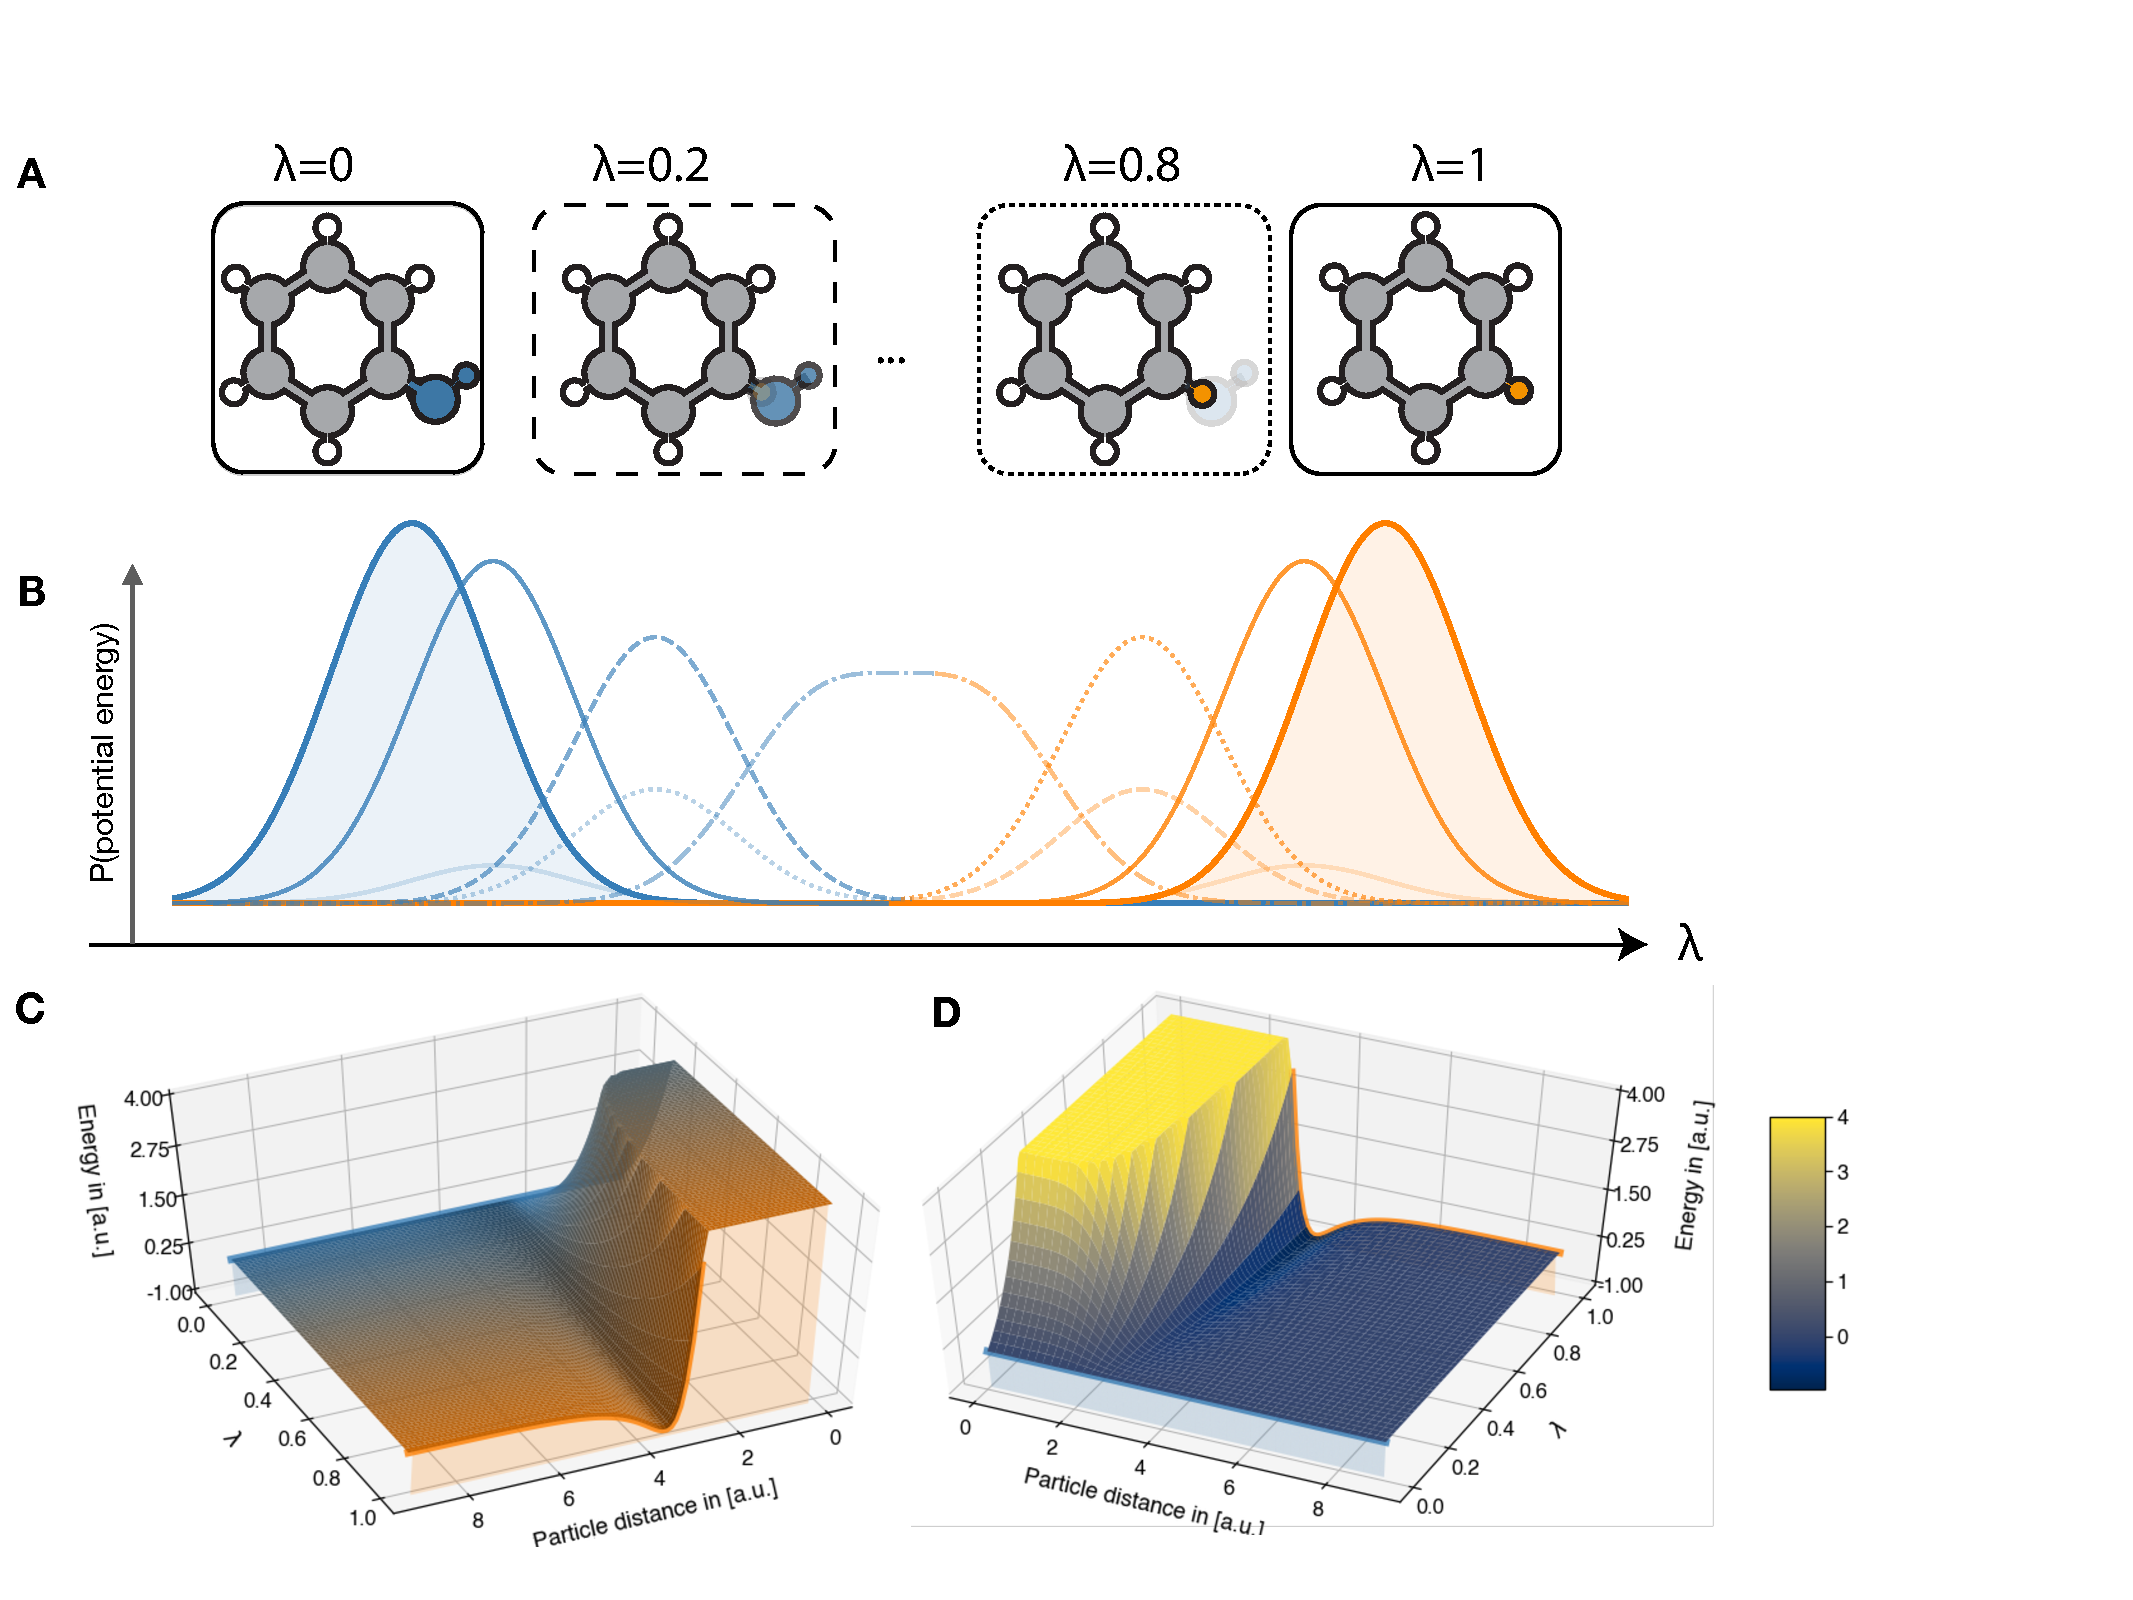
\includegraphics[width=0.95\linewidth]{figures/fig7_what_is_lam/Figure.pdf}
    \caption{Alchemical intermediates are created by making the potential energy depend on an additional variable $\vec{\lambda}$ that interpolates between the chemical endpoints. In (\textbf{A}), at $\vec{\lambda}=0$ the molecule is a fully interacting phenol and at $\vec{\lambda}=1$,  a fully interacting benzene. (\textbf{B}) shows an illustration of the probability distribution of the potential energies as the switching function takes values of $\vec{\lambda}=0$ to $\vec{\lambda}=1$. Intermediates states are required for a sufficient overlap in potential energies to estimate a free energy difference between $\vec{\lambda}=0$ and $\vec{\lambda}=1$.
    Soft-core potentials provide one of the most efficient families of intermediate pathways, with a $\vec{\lambda}$ dependence. In (\textbf{C}) the potential energy surface is coloured according to $\vec{\lambda}$ with blue being $\vec{\lambda}=0$ and $\vec{\lambda}=1$ orange. In (\textbf{D}) the potential is coloured according to the potential energy. Note how as $\vec{\lambda}$ approaches 0, the energy smoothly approaches zero at all $r$, a necessary requirement for efficient and stable calculations.  }
    \label{fig:fig_what_is_lambda}
\end{figure}

Both absolute and relative calculations must choose an alchemical pathway connecting initial and final states. In principle, because of the path independence of the free energy, any arbitrary pathway will give the correct free energy change, but the choice of pathway will greatly affect the efficiency of the calculations. Some choices are particularly crucial---for example, transformations involving insertions or deletions of atoms should employ a soft-core potential path for Lennard-Jones or other interactions with repulsive interactions that go to infinite energy at small radius~\cite{beutler1994avoiding, beutler1994molecular,gapsys2012new}.

The key consideration for choosing alchemical pathways is that the intermediate states that a given pathway produces should sample configurational ensembles that change as slowly as possible as $\vec{\lambda}$ changes, while still managing to go from the initial state to the final state as $\vec{\lambda}$ goes from 0 to 1.

Another way of stating this is that intermediate states should sample molecular configurations that are as similar as possible to their neighboring states. The more similar the configurations are between intermediate states, the lower the statistical uncertainty is in the estimate of free energy between intervals. This can be proven directly from the BAR and MBAR formulas~\cite{bennett1976efficient,klimovich2015guidelines}, though the exact same principles apply for TI. For a 'good' path to work and give a sequence of states with maximally similar configurations, sufficient similarity in potential energies is required. Fig.~\ref{fig:fig_what_is_lambda}\textbf{A} and \textbf{B} illustrate this. Fig.~\ref{fig:fig_what_is_lambda}\textbf{A} shows in a pictorial way a soft-core potential can be applied across different $\vec{\lambda}$s. Fig.~\ref{fig:fig_what_is_lambda}\textbf{B} illustrates the potential energy distributions at the different $\vec{\lambda}$ intermediates, with sufficient overlap between neighboring $\vec{\lambda}$ states to ensure that reweighting estimators such as MBAR can be used for analysis (see Sec.~\ref{subsec:estimators}). The actual transformation is best handled with soft-core potentials of the form shown in Fig.~\ref{fig:fig_what_is_lambda} \textbf{C} and \textbf{B}, with more details given below. 

So what are the options to adjust the potentials between the two end states based on $\vec{\lambda}$? The simplest possible alchemical pathway is a \textit{linear} pathway:
\begin{equation}
U(\vec{q},\vec{\lambda}) = (1-\vec{\lambda}) U_0(\vec{q}) + \vec{\lambda}U_1(\vec{q}) \end{equation},

so-called because the dependence on $\vec{\lambda}$ is linear. This clearly satisfies the basic requirement that it gives the initial endpoint potential energy $U_0(\vec{q})$ when $\vec{\lambda}=0$ and final endpoint energy $U_1(\vec{q})$ when $\vec{\lambda}=1$. 

For many energy terms this is a very good approach, \textit{as long as a repulsive core remains on}. For example, it can be shown that if van der Waals repulsions are left on, then the linear approach is very nearly the optimal path possible for changing, removing, or inserting the electrostatic energy terms, with the alchemical path being within about 10--20\% of the minimum possible uncertainty~\cite{naden2015linear} for a fixed amount of simulation time, as well as being nearly optimally efficient for van der Waals attractive terms with repulsion terms turned on~\cite{naden2014linear}. Although we are not aware of any quantitative tests for dipolar or higher multipole terms, theoretically it should behave equally well for those systems.

However, this approach ends up being terrible for removing or adding repulsive potentials that go to infinity quickly at or near the origin. One way to look at this is to examine how low $\vec{\lambda}$ values must go to reduce the energy at $0.5\sigma$ (the atomic size parameter) down to 1 $k_BT$, where thermal fluctuations make it possible for other atomic sites to penetrate routinely that deep. Assume we are trying to go from a particle being present, and desire to make it disappear alchemically. If the repulsive terms are of the form $\epsilon(\frac{\sigma}{r})^{12}$, and if $\epsilon$ is 1 $k_BT$ at the temperature of interest, and we start with the particle present, we may solve for $(1-\vec{\lambda})(1 k_B T)\left(\frac{\sigma}{0.5\sigma}\right)^{12} = 1 k_B T$. This yields $\vec{\lambda} = 1-2^{-12} \sim 0.999976$. At this point,  we have gone virtually all the way to the end of the transformation, but there is still an impenetrable post in the middle of our simulation! This is not very much like the desired final state of no interactions between the particle and its environment. We can play around with a few ways of modifying this, like simulating many more intermediate states near $\vec{\lambda}=1$. However, various analyses have shown that this is not a very good strategy~\cite{pham2011identifying, beutler1994avoiding, zacharias1994separationshifted, blondel2004ensemble, gapsys2012new}.

What we need instead is a function that smoothly gets rid of this infinity. A large number of schemes have been tried~\cite{beutler1994avoiding, zacharias1994separationshifted, blondel2004ensemble, pham2011identifying, pham2012optimal, naden2014linear, donnini2005incorporating}, but the most common strategy that appears to be the best practice is to use a "soft-core" potential, of the form:

\begin{equation}
    U(\vec{r_{ij}},\vec{\lambda}) = 4\epsilon_{ij} \vec{\lambda} \left(\frac{1}{(\alpha(1-\vec{\lambda}) + (r_{ij}/\sigma_{ij})^6)^2} -  \frac{1}{\alpha(1-\vec{\lambda}) + (r_{ij}/\sigma_{ij})^6}\right)
    \label{eq:softcore},
\end{equation}

where $r_{ij}$ is the distance between two particles $i$ and $j$, $\epsilon_{ij}$ and $\sigma_{ij}$ are the Lennard-Jones parameters corresponding to the interaction between particles $i$ and $j$, and $\alpha$ is a constant. In particular, $\alpha=0.5$ is statistically optimal for the specific functional form shown above. This functional form has exactly the property we are looking for: it recovers the Lennard-Jones potential when $\vec{\lambda}=1$, and the at other endpoint ($\vec{\lambda}=0$), it is exactly zero for all $r_{ij}$ everywhere, and as $\vec{\lambda}$ goes to zero, the $\alpha(1-\vec{\lambda})$ term lowers the infinite energy in the core. There are several different variants of the same functional form~\cite{zacharias1994separationshifted, beutler1994avoiding,pham2011identifying}, but the one given in eq.~\ref{eq:softcore} is easy to understand and implement and fairly numerically stable. This functional form is shown in \textbf{C} and \textbf{D} of Fig.~\ref{fig:fig_what_is_lambda}.

It has been shown that more complicated forms are not significantly more efficient than eq.~\ref{eq:softcore}~\cite{pham2012optimal}. We therefore recommend using the soft-core potential given in eq.~\ref{eq:softcore}, unless there is a compelling reason otherwise. Using a similar equation to eq.~\ref{eq:softcore} may be acceptable in most circumstances if that is what is supported in your chosen software. However, if you are inserting or removing entire atomic sites, we heavily recommend against using the linear approach; it will be very difficult to get correct or converged results. 

So far in this section, we have discussed optimal ways of disappearing or appearing Lennard-Jones interaction sites and turning on and off electrostatics terms. What about performing both transformations at the same time? We cannot turn off the electrostatics linearly at the same time we turn off the Lennard-Jones terms, as it would leave infinitely large attractive and repulsive electrostatic terms "bare" at small $\vec{\lambda}$, resulting in the simulation crashing. It \textit{is} possible to apply the same soft-core approach to the Coulomb interaction as to the van der Waals interaction, and this is indeed done in a number of implementations. In this case, it is important that the Coulomb interaction is softened as rapidly or more rapidly than the Lennard-Jones interaction to avoid charge penetration issues into the repulsive core, which  can be tricky to ensure for multiple types of perturbations simultaneously~\cite{steinbrecher2011softcore}. 

A safe but potentially more computationally expensive approach is to perform the transformations in sequence; first, turning off all electrostatics for atoms that must be removed, inserting and removing Lennard-Jones sites (both the insertion and removal can be done simultaneously), and then turning electrostatics for the introduced particles on. Again, if there are no removals or additions to atomic sites, then it is reasonable to change the interactions in the first and third steps  linearly. 

Other issues, such as whether absolute calculations should retain or remove intramolecular non-bonded interactions
through either annihilation~\cite{hermans1997inclusion, mann2000modeling, boresch2003absolute, wang2006absolute, mobley2006use} or decoupling~\cite{fujitani2005direct, mobley2006use}, must be considered. Reasonable efficiency can be often obtained with either choice even if some are somewhat better or worse than others, and there is no consensus on which is better in most given situations. Our recommendation is to leave the intramolecular interactions on during the transformation for simplicity if there are no other known issues with this approach. The key feature of the simulation to watch out for is whether the total potential energy, and therefore the intermediate ensembles sampled, changes smoothly from beginning to end. Problems of discontinuous changes of the potential energy can be diagnosed by noticing lack of configuration space overlap between different simulations (see Sec.~\ref{sec:are-they-good}).

Relative calculations introduce additional choices, such as the order in which to modify nonbonded interactions.
A common process in single topology relative calculations is, as noted above, to first remove electrostatic interactions of any atoms which will be deleted, then modify other non-bonded interactions, then restore electrostatic interactions of any atoms which are being inserted. Although this is a simpler path to understand cognitively and can take advantage of the soft-core potential from Eq.~\ref{eq:softcore}, this can lead to more intermediate steps and thus be more computationally expensive.
Other schemes, such as simultaneously changing electrostatic and Lennard-Jones interactions with electrostatic soft-core potentials~\cite{steinbrecher2007nonlinear}, as already discussed above, may be implemented with fewer intermediate states but could require fine-tuning of electrostatic and Lennard-Jones soft-core parameters to avoid numerical instabilities. 
At the time of writing, there has not been conclusive evidence to suggest the separate or simultaneous approach is in general better than the other, all factors considered, so discretion should be left up to the user as to what is viable from both hardware resources, and what the simulation software supports.

A key additional consideration in choosing the alchemical pathway is the choice of spacing of intermediate states.
The spacing depends to some extent on the choice of analysis method, though states should essentially be spaced equidistant in the relevant thermodynamic length~\cite{crooks2007measuring, sivak2012thermodynamic}.
For BAR/MBAR techniques this means that states should be spaced so that the statistical uncertainties between neighboring states be approximately equal~\cite{pham2012optimal, shenfeld2009minimizing}, where "approximately" is roughly within 30-50\% in magnitude. 
Some schemes to adaptively optimize the spacing of intermediate states based on initial exploratory simulations have been proposed~\cite{hayes2017adaptive}. For molecules changing in dense solvent, then the best path is roughly independent of molecule size and shape, so what works for one molecular transformation is likely to be relatively efficient for another~\cite{monroe2014converging}.


Some approaches have attempted to find alternative pathways to improve efficiency or find paths of low thermodynamic length~\cite{naden2014linear,naden2015linear,pham2012optimal}. For example, the enveloping distribution sampling (EDS) approach, and its multiple-replica and accelerated variant, works to improve efficiency by creating a single artificial intermediate state which simultaneously samples all end state phase spaces~\cite{perthold2018accelerated,sidler2017efficient, christ2007enveloping}. When this can be done, it provides an extremely efficient way to calculate the relative free energy difference between multiple ligands from a single simulation. However, it can often fail whenever the simulation of this intermediate state ends up trapped in configurations characteristic of only one end state. Thus, successful use of EDS can require system-dependent tuning, making it difficult to implement in an automated and reliable way. However, when successful, it can be very efficient.

In our view, there is still some room for further exploration of how to best choose transformation pathways, especially for relative binding calculations or more complex molecules, as most existing studies focus on smaller molecules. As we have stressed, in principle, any pathway that connects the desired end states is rigorously correct, but as discussed above, different paths may differ dramatically in thermodynamic length and therefore efficiency. Additionally, some paths simply may not converge due to issues noted above such as those encountered without soft core potentials. However, the recommendations above are reasonable, reliable, and are likely not that much less efficient than potentially more optimal choices~\cite{naden2014linear,naden2015linear,pham2012optimal}, as the real problems with the efficiency of calculating free energies are lack of sampling of slow conformational modes, rather than the lack of efficiency of the transformations. 

It is however important to note that different packages also differ in how they handle implementation of alchemical transformations, making it difficult to give rules of thumb concerning specific efficient transformations which work equally well across simulation packages. Thus, we are hesitant to recommend best practices within specific software packages at this point in time, although any good transformation pathway will conform to the guidelines we have outlined above.


\subsubsection{Which sampling scheme will work best for my problem?}
\label{sec:sampling_schemes}
Though all alchemical simulations must sample from multiple $\vec{\lambda}$ states, different approaches can be used to achieve this. Fig.~\ref{fig:fig_sampling_scheme} illustrates the four most common schemes. The simplest approach involves running an independent simulation at each of the predefined $\vec{\lambda}$ values (see Fig.~\ref{fig:fig_sampling_scheme}\textbf{A}). This type of scheme is currently used for AMBER TI calculations~\cite{song2019using} and for Sire as implemented in BioSimSpace~\cite{hedges2019biosimspace}. However, if these simulations can be run simultaneously with communication between them, a simple extension allows mixing between these replicas. In this approach, the simulation at each $\vec{\lambda}$ can undergo periodic exchanges with neighboring $\vec{\lambda}$ values. This form of replica exchange, called Hamiltonian replica exchange, is based on ideas developed from Monte Carlo simulations of spin glasses by Swendsen and Wang~\cite{swendsen1986replica}. With the Metropolis-Hastings acceptance criterion for exchanges, the generated ensemble of all replicas still samples from the Boltzmann distribution for each replica. This approach has been used in many different contexts for molecular simulations~\cite{sugita2000multidimensional,sugita1999replicaexchange, woods2003development, jiang2010free}. The basic idea of the replica exchange scheme is shown in Fig.~\ref{fig:fig_sampling_scheme}\textbf{B}. It is supported in various software packages that provide alchemical implementations, such as GROMACS~\cite{aldeghi2015accurate}, GROMOS~\cite{hritz2008hamiltonian,hritz2007optimization}, FEP+~\cite{wang2015accurate}, and NAMD~\cite{jiang2019computing}. 

A third approach borrows ideas from simulated tempering~\cite{marinari1992simulated}. In this scheme a single replica rapidly explores all of $\vec{\lambda}$ space by working out optimal weights that allow switching between different intermediate $\vec{\lambda}$ values, as seen in Fig.~\ref{fig:fig_sampling_scheme}\textbf{C} . This approach is also referred to as self-adjusted mixture sampling~\cite{lyubartsev1992new, li2007simulated, tan2017optimally} and while promising, has so far only been supported in OpenMM Tools~\cite{andrearizzi2019choderalab} and GROMACS.  Although this approach allows multiple states to be simulated in a single simulation, the weights do not always converge to the proper equilibrium distribution, and care must be taken that the final results are converged. 

The last approach makes use of non-equilibrium simulations~\cite{aldeghi2018accurate}. In this approach, only end state $\vec{\lambda}$ replicas ($\vec{\lambda}$=0, $\vec{\lambda}=1$) are simulated at equilibrium; intermediate information is generated from non-equilibrium simulations that rapidly transition between end states. This approach is available in GROMACS and appears to be coming online in several other packages. A schematic of this approach is shown in Fig.~\ref{fig:fig_sampling_scheme}\textbf{D}. 

\begin{figure}
    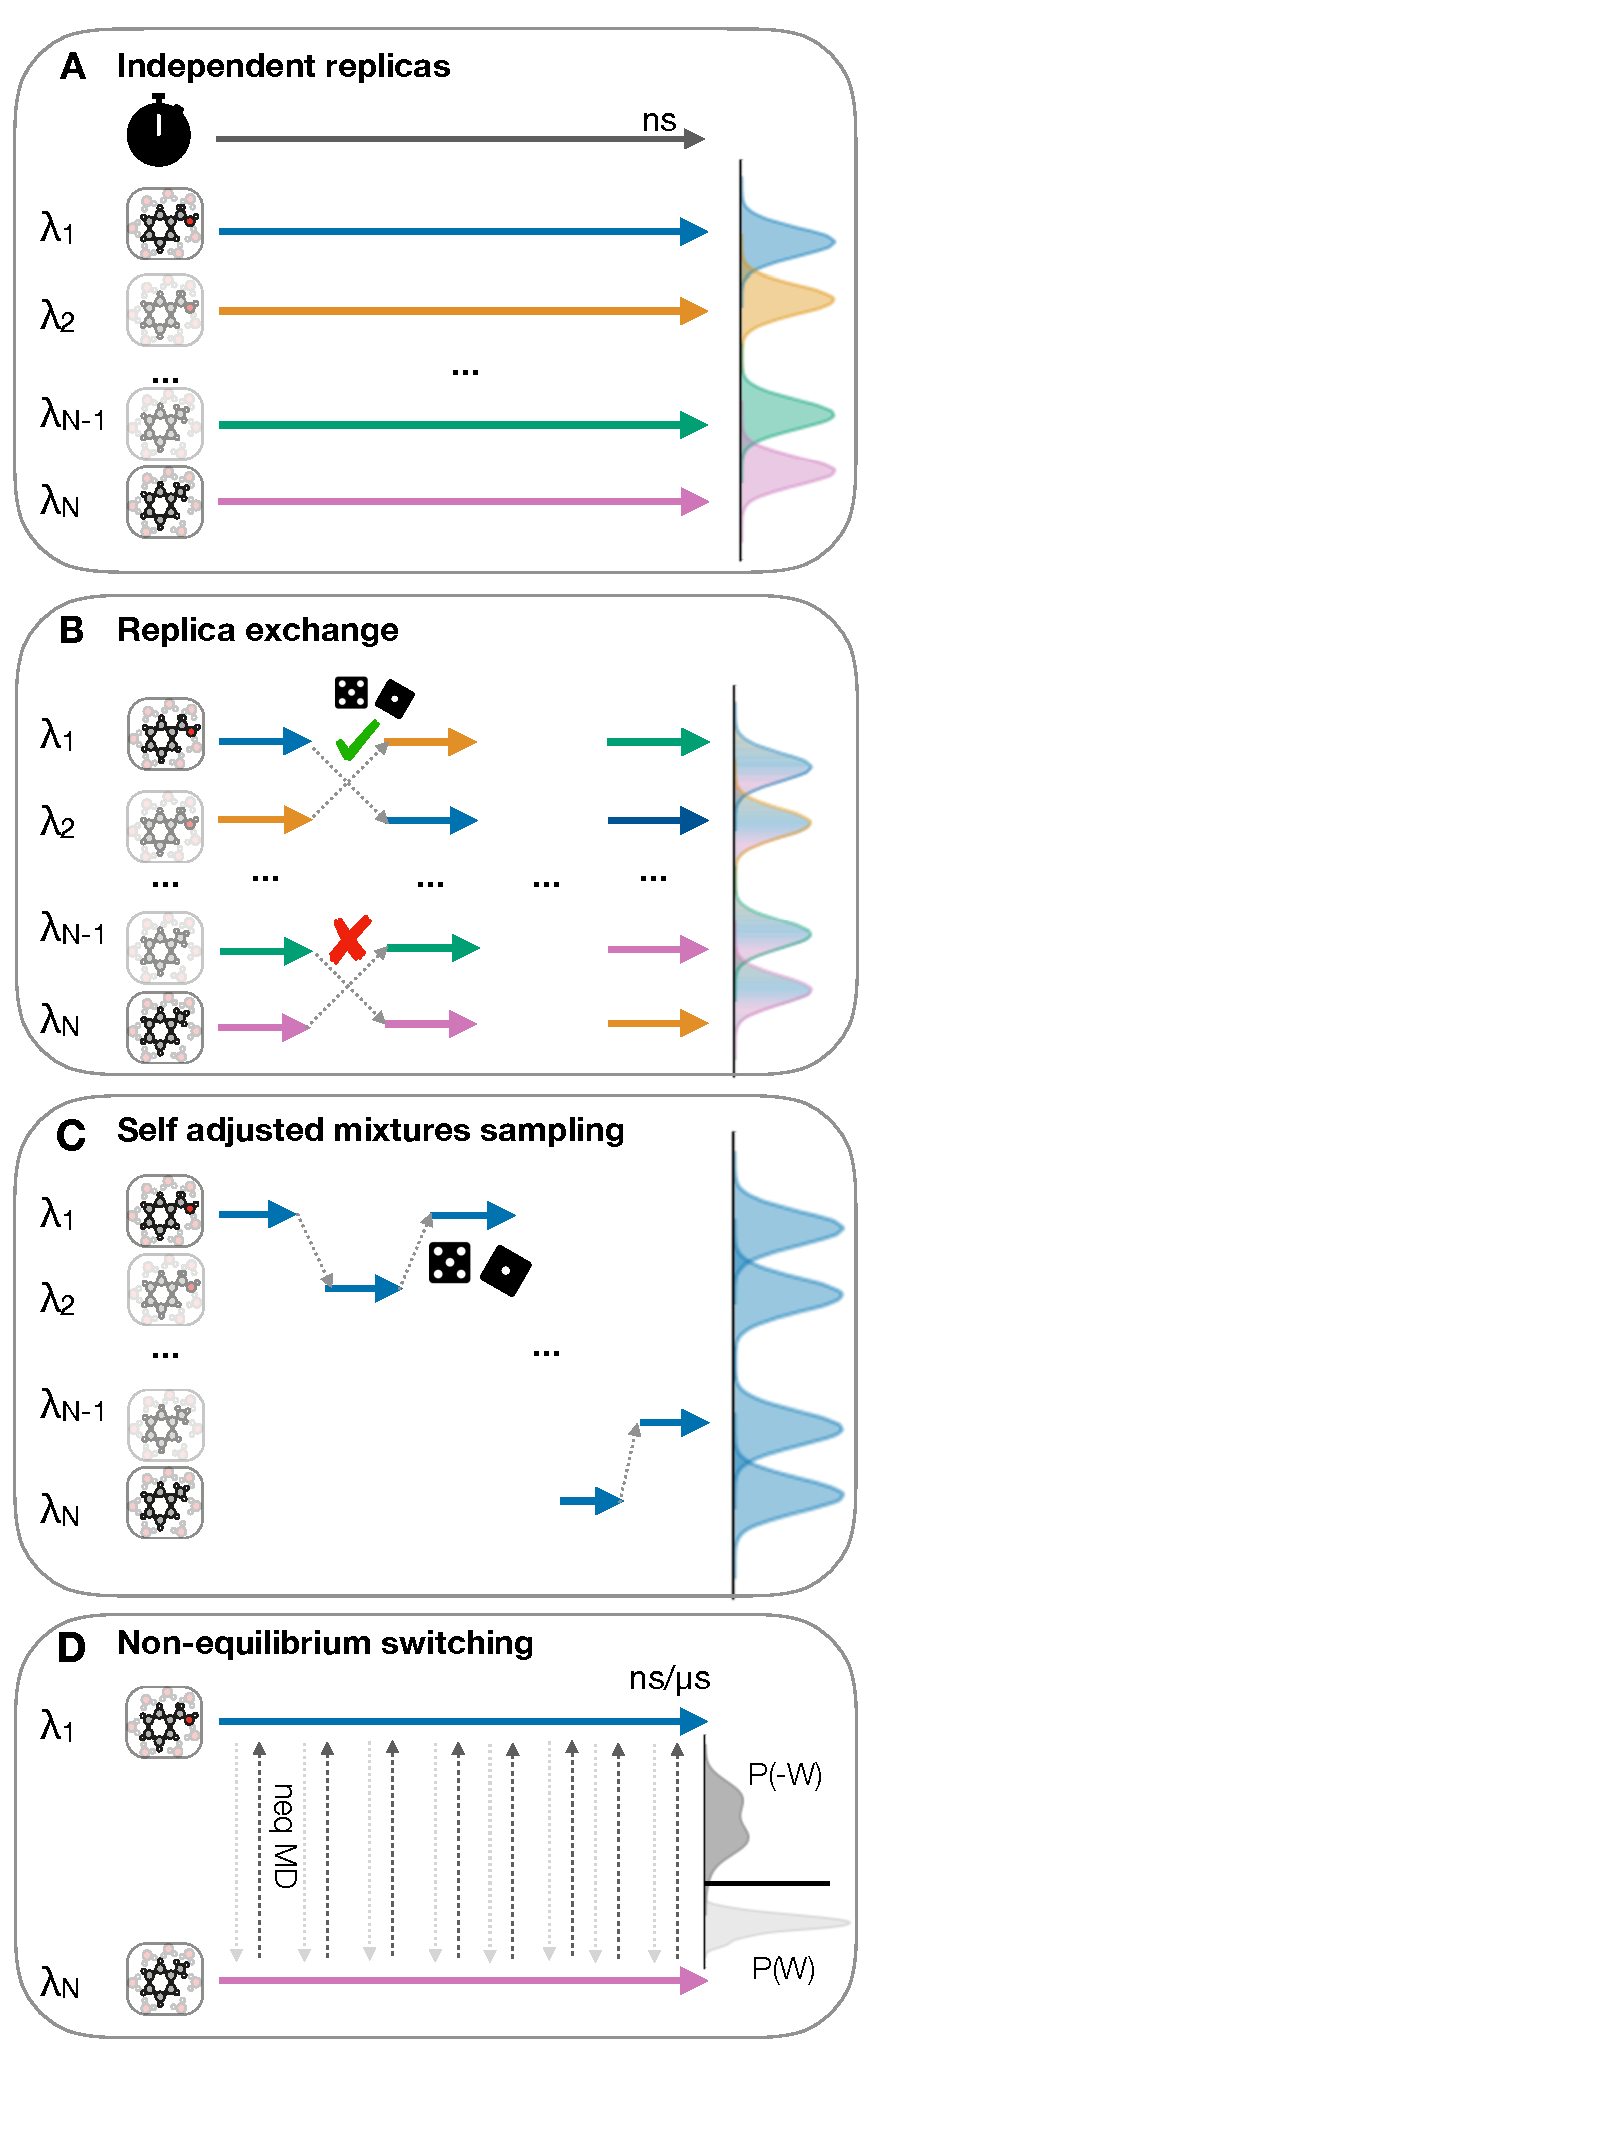
\includegraphics[width=0.88\columnwidth]{figures/fig8_sampl_scheme/Figure.pdf}
    \caption{\textbf{Four most common sampling strategies.} (\textbf{A}): Multiple replicas in parallel at different lambda states. Each arrow symbolises an independent $\vec{\lambda}$ simulation. (\textbf{B}): Hamiltonian replica exchange scheme. Each arrow represents a short simulation interval before an exchange through Metropolis Hastings acceptance (dice) is attempted. A tick means an accepted exchange, a cross a rejected exchange. (\textbf{C}): Single replica scheme sampling from all $\vec{\lambda}$ states. After a short simulation time symbolised by the arrow, the lambda-state is attempted to change until all N lambda states will be sampled. (\textbf{D}): Non-equilibrium sampling scheme, where two equilibrium simulations at the end states are run as indicated by the blue and pink arrow. Non-equilibrium simulations are attempted at intervals to switch between the two end states.}
    \label{fig:fig_sampling_scheme}
\end{figure} 

Currently, we recommend using Hamiltonian replica exchange type sampling schemes (Fig.~\ref{fig:fig_sampling_scheme} \textbf{B}). If these are not available in the code of choice, running independent simulations at different $\vec{\lambda}$ values can be acceptable, especially when configurational sampling is fast (Fig.~\ref{fig:fig_sampling_scheme} \textbf{A}). Single replica schemes and non-equilibrium schemes are not as established yet because of potential failure modes, but are very promising for use in the near future. 


\subsubsection{How long should I run my simulation for and what information should be saved?}
\label{sec:sim_length_information_kept}
Before launching alchemical free energy calculations it is wise to consider how convergence and completion will be assessed. Different conditions on when to stop alchemical free energy calculations should be determined, and this may require several iterative checks and therefore modifications to the calculation protocol.
One useful metric to use for termination is the expected or desired uncertainty of a desired free energy estimate, though care must be exercised should the uncertainty estimate prove unreliable.
In particular, if the rate of change in the free energy estimate is significant when this condition is met, the simulation may not be locally converged, and more sampling may be necessary to determine a stable free energy estimate which is no longer changing significantly over time. 


However, this is not the only metric which can or should be used, as the uncertainty only captures the information about the sampled phase space, not necessarily the entirety of the phase space.  
For example, convergence of relative free energy calculations in predictive simulations where the entire phase space is not known in advance, requires sampling the different kinetically stable states~\cite{mobley2012perspective}. 
This highlights the importance of choosing the correct thermodynamic path to ensure you sample the required thermodynamic states as discussed in Sec.~\ref{sec:important_path}.

The condition of minimizing the statistical uncertainty of different free energy estimators below a sufficient threshold should be one metric monitored over the simulation. This can be done through the uncertainty estimator built into certain analysis tools such as MBAR, or through more general statistical tools like bootstrap sampling. It should be noted however, that uncertainty estimates have the same limitations as other metrics of convergence, as they are only an uncertainty based on the phase space sampled so far in a simulation, and cannot account for states not sampled, and it is worth considering that they will be an underestimation of the true uncertainty.
A target statistical uncertainty should be chosen at the onset of the simulation to avoid excessively long simulations, or falling into the trap of running until the free energy estimate is "good enough," which is subjective and has no defined criteria. This could be a fixed value such as $0.20$ kcal/mol, or a functional quantity such as "below $0.5$ kcal/mol and $10\%$ of the free energy estimate." The user does not need to monitor this information in real-time and can choose to run simulations for fixed duration (either time or number of samples) and run analysis on the data collected thus far. If more samples are needed, the simulations can be resumed, or, started again in different initial conditions. 

Convergence in other alchemical observables should also be monitored to determine if the defined phase space has been sufficiently sampled and enough decorrelated samples have been drawn. These additional observables include, but are not limited to, the variance in $\frac{dU}{d\vec{\lambda}}$ across all $\vec{\lambda}$ values, calculating the variance in free energy using bootstrap analysis, and comparing differences in free energies calculated using different percentages of the simulation in both the forward and reverse directions~\cite{klimovich2015guidelines} (see Fig.~\ref{fig:convergence_forward_reverse}).

\begin{figure}
    \centering
    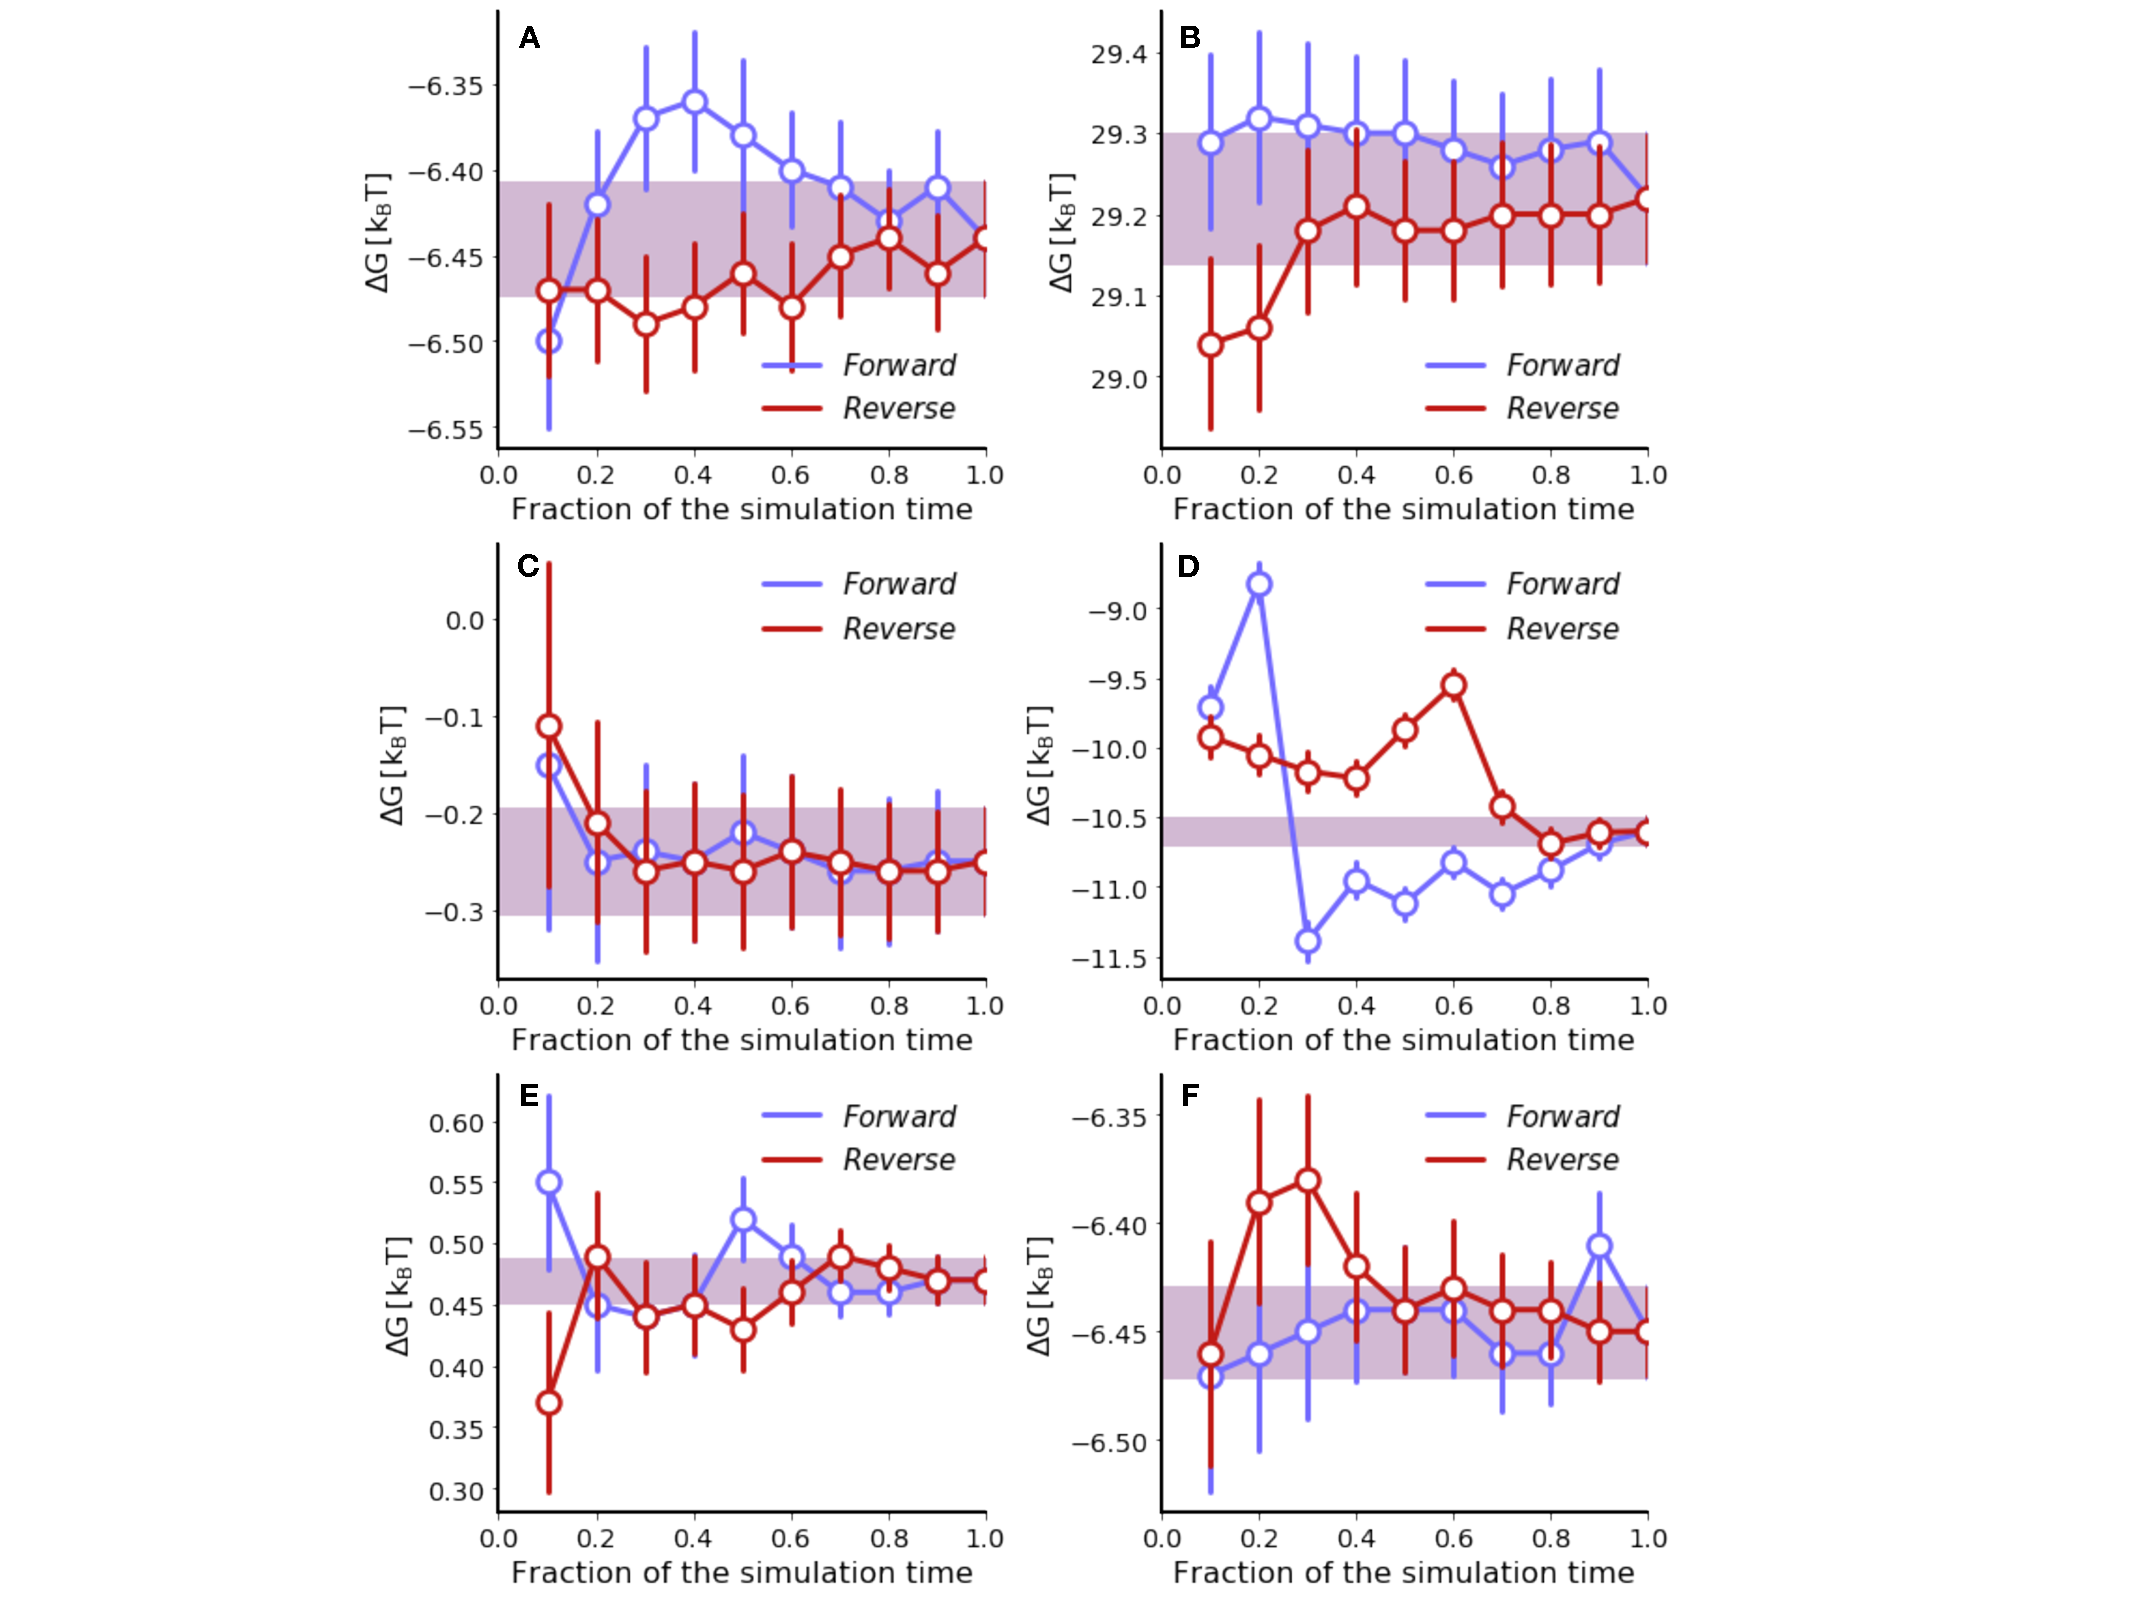
\includegraphics[width=0.95\linewidth]{figures/fig10_forward_reverse/Figure.pdf}
    \caption{\textbf{Free energy (in $k_{B}T$) for two different relative binding free energy perturbations.} 
    Each plot shows the estimated free energy change using a varying fraction of total simulation time (up to 5 ns total). 
    Subplots (\textbf{A}), (\textbf{C}), and (\textbf{E}) show a three step protocol for a perturbation involving 3 perturbed atoms, while (\textbf{B}), (\textbf{D}), and (\textbf{F}) shows the same protocol for a perturbation involving 10 perturbed atoms. The first step of the protocol is the decharging then removing van der Waals interactions and then recharging. The difference in energy between the forward (blue) and reverse (red) free energy calculations at the midpoint of the simulation time gives an indication of the overall convergence of the simulation, with differences over 1 $k_{B}T$ indicating poor convergence.}
    \label{fig:convergence_forward_reverse}
\end{figure}

Each of these metrics shows some promise for diagnosing when a simulation has a convergence issue beyond simple convergence of uncertainty estimates. 
Results obtained from calculations with convergence issues should be checked for errors or run for longer before any confidence should be placed in conclusions drawn from their analysis.
For example, in relative calculations ligands that share similar binding modes and do not induce large conformational changes when in complex with protein, the need to sample exhaustively to converge estimates in free energy differences is often minimal due to the locality of sampling changes in the molecular topology and shared phase space of the core atoms.
However, even subtle induced changes in protein binding configuration will require more sampling or cause local convergence to a free energy estimate that has high error.
The confidence a user should have in a free energy estimate is significantly improved when both the uncertainty of the free energy estimate is low, and when other observables have reached a convergence.

\begin{figure}
    \centering
    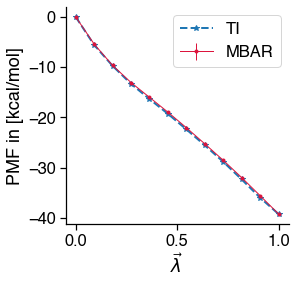
\includegraphics[width=0.8\linewidth]{figures/fig_pmf/pmf.png}
    \caption{{\bf Potential of mean force with respect to $\vec{\lambda}$ for TI and MBAR}
    The estimated PMF for a bound calculation of a Tyk2 ligand pair of Wang et al.~\cite{wang2015accurate} with respect to $\vec{\lambda}$ estimated from TI and MBAR and showing agreement within errorbars. 
    }
    \label{fig:pmf}
\end{figure}

The uncertainty in the free energy, for example, can be estimated in multiple ways, e.g. through standard error propagation methods (including MBAR's estimator, which is based on the same principles as standard error propagation), through bootstrap methods, and through multiple independent runs. 
Independent of how the property is estimated, it is important to remember that results of any free energy analysis are \textit{estimations of the given property}, not the true underlying value of the property itself. 
These estimators are usually consistent estimators, meaning they will converge to the true answer in the limit of sufficient sampling, not necessarily unbiased ones though.
As such, it is a good idea to subject different estimators to the same data to see if they yield either the same estimate (within error and bias), or if they fluctuate wildly. See, for example, the potential of mean force with respect to $\vec{\lambda}$ estimated from a bound simulation of a Tyk2 ligand pair of Wang et al.~\cite{wang2015accurate} for both the MBAR and TI estimators, as seen in Fig.~\ref{fig:pmf}.
This is not a perfect method as some estimators, such as exponential averaging, will converge significantly more slowly, relative to more accurate estimators like MBAR. 
Therefore, it is a good idea to apply the estimators to different fractions of the data to see if the main estimator of free energy you have chosen is stable.

Each method requires different data from the simulation be collected. If, for instance, the free energy estimator selected is thermodynamic integration, then values of $\frac{dU}{d\vec{\lambda}}$ at uncorrelated data points must be collected. Once you have made a choice of the combination of the type of simulation you will run, which alchemical topology you will simulate, what alchemical path you will simulate along, and what your stopping conditions are, then you are ready to enumerate the information you should capture. Below is a sample of the minimal information you need for a set of common estimators (discussed in more detail in Sec.~\ref{subsec:estimators}):

\begin{itemize}
    \item Thermodynamic Integration (TI) requires $\frac{\partial u(\vec{q})}{\partial\vec{\lambda}}$.
    \item Exponential Averaging (EXP) needs \textit{either} $\Delta u_{k,k+1}(\vec{q})$ or $\Delta u_{k,k-1}(\vec{q})$, depending on the direction its being evaluated in.
    \item Bennett Acceptance Ratio (BAR) needs \textit{both} $\Delta u_{k,k+1}(\vec{q})$ and $\Delta u_{k,k-1}(\vec{q})$.
    \item Weighted Histogram Analysis Method (WHAM) and Multistate Bennett Acceptance Ratio (MBAR) both need the complete set of $\Delta u_{k,j} \, \forall \, j=\{1...K\}$. WHAM must have this same information binned with some choice of bin width small enough not to affect the results.
\end{itemize}

The potential derivative required for TI should generally be calculated during the simulation; only under very rare circumstances~\cite{naden2015linear} can it post-processed by a code that does not evaluate the derivatives. Many codes already have options for doing this.
If that option is unavailable, you can estimate it through finite difference (if sufficient information is collected), but this will introduce significant error, and is generally not a best practice. The BAR estimator may be a better, and simpler choice at that point as you will have at least the same level of information. 

The potential energy differences required for EXP, BAR, MBAR, and WHAM can be calculated either during the simulation or in post-processing. It is recommended to calculate the potential differences in code when possible to avoid extra overhead and possible errors produced by evaluating the energy of the configuration twice, and to reduce the amount of stored information. 
Although potential energy derivatives must usually be calculated in code there is one condition under which they can be easily computed in post-simulation analysis. 
If the alchemical path you have chosen is a linear alchemical path, then $\frac{du}{d\vec{\lambda}} = u_0(\vec{q}) - u_1(\vec{q})$, which is the difference between the initial and final states, which are already calculated by the simulation and can be recorded easily without additional computational expense. 
However, because of the problems with linear paths already discussed in this paper, this simplification is rarely that useful.


Free energy information should generally be saved more frequently than coordinate data, approximately at the rate that uncorrelated samples are produced.  
The on-disk size of the data for free energy estimation is often significantly smaller than full atomic coordinates, so the information can easily be collected frequently. 
However, the information should not be collected \textit{every} time step, as most free energy techniques are operated at equilibrium, and need equilibrated \textit{and decorrelated} samples for an unbiased estimate.
Samples collected every time step will likely result in most samples being discarded due to the detection of correlation in the time series by decorrelation routines in the analysis. However, if it is computationally cheap and disk space is plentiful, do save often. One may safely assume that the correlation time is greater than 100-200 fs even for relatively simple systems such as small molecules in solvent, so saving no more frequently than every 50-100 steps is recommended. 
How decorrelation impacts calculations, and how to compute it is discussed in Sec.~\ref{sec:decorrelating-samples}.

In general, uncertainties can be assumed to decrease as $1/\sqrt(N)$ where $N$ is the number of uncorrelated samples, for all standard free energy calculation methods~\cite{shirts2005comparison}. However, this carries the notable caveat that such estimates require accurate estimation of the correlation time which, if important motions are slow compared to simulation timescales, can be difficult. Still, this metric provides a good rule of thumb, and as long as conformational transitions are captured by the simulation, increasing the aggregate simulation time by a factor of $T$ will reduce the uncertainty by a factor of approximately $\sqrt{T}$.

\subsubsection{Multiple or uncertain binding modes may require considerable care}
\tocsubsubsectioncomment{@Michael Shirts to update discussion of treatment of multiple binding poses.}
\label{sec:multiple_binding_modes}
In a discovery setting, new ligands can have unknown or at least uncertain binding modes~\cite{kaus2015how, plountprice2000analysis,mobley2009binding,calabro2016elucidation}, complicating binding free energy estimation.

To deal with prospective ligands with unknown binding modes, discovery projects commonly assume that modifications of functional groups on a common scaffold result in a consistent binding mode across all members of a series.
This is not necessarily always the case~\cite{kaus2015how}, as reviewed elsewhere~\cite{mobley2009binding} and in some cases unexpected binding mode changes can be the origin of apparent non-additivity in structure-activity relationships~\cite{calabro2016elucidation}.
Binding modes also tend to be particularly variable in the case of fragments, which often may have multiple relevant binding modes~\cite{steinbrecher2015accurate}.


Absolute free energy calculations for dissimilar ligands can have particular challenges because the (potentially incorrect) assumption of consistent binding modes across a series of similar ligands is likely to be even less robust than in the case of relative calculations.
This means that researchers performing absolute binding free energy calculations will have to pay particular attention to generating reasonable putative binding modes.

In some cases, it is tempting to simply use docking techniques to generate initial bound structures for starting molecular dynamics simulations.
However, timescales for binding mode interconversion are usually slow compared to MD/free energy timescales, meaning that simulations started from different potential binding modes are likely to yield disparate computed binding free energies~\cite{mobley2006use, palma2012computation, mobley2012perspective, gill2018binding}. Moreover, docking techniques are good at identifying sterically reasonable potential binding modes, but still perform relatively poorly at identifying a single dominant binding mode \emph{a priori}. 


It is worth highlighting a recent SAMPL blind challenge on HIV integrase as an illustration of this. 
Many submissions, using state-of-the-art methods, had difficulty even predicting which \emph{binding site} ligands would bind in---most submissions placed more than half of the ligands into the incorrect binding site---and even given correct binding sites, the binding mode within each site was also quite difficult to predict~\cite{mobley2014blind}.
The best performing submission for predicting binding modes actually ended up being a human expert (aided by computational tools) with more than 10 years of experience on the particular target~\cite{voet2014combining}, rather than a fully automated approach.
While free energy calculations on this set had some success, many of the failures actually ended up being cases where the binding mode selected as input for free energy calculations was later found to be incorrect~\cite{gallicchio2014virtual}, highlighting the importance of these issues.

One approach which has shown some success in identifying accurate binding modes \emph{de novo} is to retain diverse potential binding modes from docking, perform short MD simulations of these to identify distinct stable binding modes, and then consider only these stable modes in subsequent calculations~\cite{gallicchio2014virtual, mobley2006use,rocklin2013blind, boyce2009predicting, mobley2007predicting}.


Routes to handle multiple potential binding modes are different depending on whether absolute or relative calculations are selected, unless a method is available to estimate the relative populations of different stable binding modes in advance (e.g. such as the BLUES approach currently in development~\cite{gill2018binding}), in which case this approach could be applied to assist both types of calculations.

\paragraph{Handling multiple potential binding modes within absolute calculations.}
Within absolute binding free energy calculations, multiple potential binding modes can be handled by two main strategies: Considering each binding mode separately (a separation of states strategy) or sampling all binding modes within a single simulation~\cite{mobley2012perspective}.
This couples to the choice of restraints selected, as some restraints will allow transitions between binding modes and even binding sites (Sec.~\ref{sec:standardstate-restraints}), and others do not.

Sampling all potential ligand binding modes within a single free energy calculation is usually impractical without some form of enhanced sampling or at least Hamiltonian replica exchange~\cite{wang2013identifying} because barriers for binding mode interconversion result in kinetics which are too slow compared to simulation timescales~\cite{mobley2006use, palma2012computation,mobley2012perspective, gill2018binding}.
Hamiltonian exchange, coupled with appropriate restraints, can allow the ligand to relatively rapidly exchange between potential binding modes when non-interacting, accelerating sampling of binding modes~\cite{wang2013identifying}. However, it is not always clear that this is desirable, since this also increases the size of the configuration space which must be sampled even if the binding mode is known.

Separation of states provides a simple though potentially expensive alternative, where each stable binding mode is considered separately with a binding free energy calculation restricted to that binding mode, and then (as long as the binding modes are non-overlapping) the resulting component binding free energies can be combined into a total~\cite{mobley2006use, mobley2012perspective}.
This approach necessitates a separate binding free energy calculation for each potential binding mode, however, so it can be computationally quite costly.
If relative populations of different stable binding modes were available from some other technique, it could make this separation of states approach considerably more efficient~\cite{mobley2012perspective, gill2018binding}.

\paragraph{Handling multiple potential binding modes within relative calculations.}
Multiple potential binding modes pose particular problems for relative free energy calculations, as having multiple starting structures for these calculations could yield substantially different calculated relative binding free energies for the same transformation due to kinetic trapping, and, without additional information (specifically, the free energy of binding mode interconversion or, equivalently, the relative populations of different binding modes) it becomes impossible to sort out which of the multiple answers is in fact the correct relative binding free energy.

To deal with this, some practitioners have actually computed relative binding free energies of different binding modes of the same ligand~\cite{palma2012computation}.
For example, a perturbation which adds a methyl to an aromatic ring of a larger ligand might yield one result if the methyl points in one direction, and a different value if it points in the other due to slow ring motions~\cite{lincoff2016comparing, sasmal2020sampling}.
One could compute the free energy of turning off the methyl group in one orientation and turning it back on in the other orientation to obtain the free energy difference between the two potential binding modes.
While this approach has precedent, it is relatively difficult to automate at present and requires considerable care.

Overall, this likely means that relative free energy calculations will be susceptible to problems resulting from uncertainty in ligand binding modes until more robust approaches are available to determine dominant binding modes, or the relative populations of different potential binding modes, in advance.

\subsection{Absolute and Relative Binding Free Energies with Multiple Chemical States}

Consider, as an illustration, the binding equilibrium between a receptor $R$ and a ligand $A$ that exists in solution as a mixture of protonated $AH$ and ionized $A^-$ forms. It is often useful to consider the observed equilibrium binding constant between $R$ and the $A$ mixture 
\begin{equation}
  K_b(A) = C^\circ \frac{[RA]}{[R][A]}
  \label{eqn:observed-binding-constant}
\end{equation}
where $[A] = [AH] + [A^-]$ and $[RA] = [RAH] + [RA^-]$ are the total equilibrium concentrations of free $A$ and receptor-ligand complexes. The observed equilibrium constant is significant because it corresponds to binding affinity measurements that do not distinguish between the protonation states of the ligand. Inserting the definitions of $[A]$ and $[RA]$ in Eq.~(\ref{eqn:observed-binding-constant}), splitting the sum in the numerator, and multiplying and dividing each term by either $[AH]$ or $[A^-]$ we obtain
\begin{equation}
  K_b(A) = \frac{[AH]}{[A]}  K_b(AH) +  \frac{[A^-]}{[A]} K_b(A^-) =  p_0(AH) K_b(AH) +  p_0(A-) K_b(A^-)
  \label{eqn:observed-binding-constant-split}
\end{equation}
where
\begin{equation}
  K_b(AH) = C^\circ \frac{[RAH]}{[R][AH]}
  \label{eqn:observed-binding-constant-prot}
\end{equation}
is the specific equilibrium binding constant between the receptor and the protonated form of the ligand, and similarly for $K_b(A^-)$. The specific $K_b$'s are the binding constants that would be obtained from ABFE calculations for those species. Eq.~(\ref{eqn:observed-binding-constant-prot}) states that the observed binding constant is an average of the specific binding constants weighted by the populations, $p_0(AH)$ and  $p_0(A^-)$ of each ligand's chemical form in solution. In this specific example, if the $pKa$ of $AH$ is known and $\alpha = [A^-]/[AH] = 10^{pH-pKa} $ is ionization ratio of $A$ at a a given $pH$, the populations of the ionized and protonated forms are $p_0(A^-) = \alpha/(\alpha+1)$ and $p_0(AH) = 1/(\alpha+1)$, respectively.\cite{champion2024multistate,azimi2022application}

Eq.~(\ref{eqn:observed-binding-constant-split}) is a particular case of a fundamental result that extends to an arbitrary number of chemical forms of a ligand in solution. In general, the observed binding constant of a ligand present in solution in multiple forms $A_i$ (protomers, tautomers, rotamers, etc.) with populations $p_0(A_i)$ is\cite{khuttan2023taming}
\begin{equation}
  K_b(A) = \sum_i p_0(A_i) K_b(A_i)
  \label{eqn:observed-binding-constant-general}
\end{equation}
and the corresponding standard binding free energy is
\begin{equation}
 \Delta G^\circ_b(A) = -k_B T \ln K_b(A) = -k_B T \ln \sum_i p_0(A_i) e^{-\Delta G^\circ_b(A_i)/k_B T}
  \label{eqn:observed-binding-free-energy-general}
\end{equation}
where
\begin{equation}
\Delta G^\circ_b(A_i) = -k_B T \ln K_b(A_i)
\end{equation}
is the standard binding free energy of the specific form $A_i$. Eq.~(\ref{eqn:observed-binding-constant-general}) is known as the free energy combination formula, which, in the case of multiple conformational states, can be derived directly from the statistical mechanics definition Eq.~(\ref{eq:DG0-binding-constant-def}).\cite{jayachandran2006parallelized,gallicchio2011recent} It states that the contribution of a chemical or conformational state of the ligand to the observed binding free energy depends on the specific binding free energy of that state and its solution population. A state with a strong specific binding affinity may not contribute significantly to the observed binding free energy if its solution concentration is low. Conversely, a sparsely populated ligand state in solution could be responsible for most of the observed binding free energy if its binding affinity is sufficiently strong relative to the other states.\cite{azimi2022application}   

The result of Eq.~(\ref{eqn:observed-binding-constant-general}), which applies to absolute binding free energy calculations, extends to relative binding free energies or, equivalently, to ratios of observed binding constants for the same receptor of two ligands $A$ and $B$ present in solution in multiple chemical forms:
\begin{equation}
  \frac{K_b(B)}{K_b(A)} = \frac{\sum_i p_0(B_i) K_b(B_i)}{\sum_i p_0(A_i) K_b(A_i)}
  \label{eqn:observed-binding-constant-ratio}
\end{equation}
The result above can be expressed in a more computationally tractable form by separating out from the numerator and denominator the specific binding constant of a reference form of each ligand ($A_0$ and $B_0$) to obtain\cite{de2018rigorous}
\begin{equation}
 \frac{K_b(B)}{K_b(A)} = \frac{K_b(B_0)}{K_b(A_0)} \frac{
 p_0(B_0) + \sum_{i=1} p_0(B_i) K_b(B_i)/K_b(B_0)
 }{
p_0(A_0) + \sum_{i=1} p_0(A_i) K_b(A_i)/K_b(A_0)
 }
\end{equation}
which involves only quantities obtainable by relative binding free energy calculations--one for the two reference forms of the ligand to get  $K_b(B_0)/K_b(A_0)$ and those of each form of each ligand relative to the reference to get $K_b(B_i)/K_b(B_0)$ and $K_b(A_i)/K_b(A_0)$.

\subsection{General simulation setting choices that could affect free energy calculations.}
\tocsubsectioncomment{@Volunteer: Add short discussion of recommended integrators? BAOAB?}
There are many parameter choices that are common to standard MD simulations. Optimal choices may depend on the simulation package and it is best to consult the manual of each package to make the right choices. One particular parameter we want to draw attention to which is often overlooked is the timestep. The choice of integrator can drastically affect the accuracy of a given calculation depending on the timestep~\cite{leimkuhler2016efficient}. Using a 1.0 fs timestep near the limit of stability without any constraints can lead to non-negligible statistical mechanical errors. However, from various previous free energy studies using 1 fs integration timesteps it is not clear that a significant error would be introduced into a free energy estimate and may warrant some further investigation.  

%%%%%%%%%%%%%%%%%%%%%%%%%%%%%%%%
%  Data Analysis               %
%%%%%%%%%%%%%%%%%%%%%%%%%%%%%%%%
\section{\tocorange{Data analysis}}
\label{sec:data_analysis}
Once equilibrium data has been collected from alchemical intermediates, it must be analyzed to produce an estimate of the free energy change (and its associated statistical uncertainty) for each leg of the thermodynamic cycle.
While a number of different estimators are available that will give consistent results under optimal circumstances, some approaches are recommended over others due to their robustness and ability to provide information on poor convergence.

\subsection{Estimators for free energy differences}
\label{subsec:estimators}
Free energy differences between two different states differing in the energy function are directly related to the
ratio of probabilities of those states.
As can be noted, the partition functions in Eq.~\ref{eq:conf_probability} are simply the total accumulated probabilities for all possible configurations of the system. Virtually all of the ways to estimate this free energy are based in converting this ratio of integrals to something that can be measured in one (or several) simulations.  

\paragraph{The Zwanzig relationship (EXP)}
The simplest method for calculating free energy differences from simulations is the so-called \textit{Zwanzig
relationship}~\cite{zwanzig1954hightemperature}, also called one-sided exponential re-weighting (EXP), or simply free energy perturbation, though this final term is sometimes used to encompass all ways of calculating free energy differences.

The (reduced) free energy difference $\Delta f_{01}$ between an initial state 0 and a final state 1 defined by two different potential energy functions 
$u_0(\vec{q})$ and $u_1(\vec{q})$ over coordinate space $\vec{q}$ can be calculated as:
\begin{eqnarray}
\Delta f_{01} & = & -\ln \expect{e^{-(u_1(\vec{q}) - u_0(\vec{q}))}}_0 =  -\ln \expect{e^{-\Delta u(\vec{q})} }_0
\end{eqnarray}\label{eqn.zwanzig}
and the average is over all samples from the simulation performed with $u_0$. In the case of NVT (canonical) sampling and assuming the masses do not change, then $u$ is simply $U/k_BT$, and $f$ is $F/k_BT$, but it can be generalized to other ensembles with the proper definition of $f$ and $u$.
Described in words, we take the samples generated during our run with the potential energy function $u_0(\vec{q})$ and calculate what the difference in energy would be if we switched instantaneously to the potential energy function $u_1(\vec{q})$, and average the exponential of the negative energy difference to get the negative of the exponential of the free energy difference. The original distributions, P($u_0$) as generated at $\vec{\lambda}=0$ and P($u_1$) would look like those seen in Fig.~\ref{fig:fig_sampling_scheme}\textbf{A}-\textbf{C} on the right hand side. Reevaluating requires almost no extra code functionality to perform; one need only to save a full precision trajectory, and run an unmodified molecular simulation code using the $u_1$ in order to calculate the new energies of stored snapshots. The analysis can be written in a line of code. We note that this method is even more general, in that the instantaneous work to change the potential energy function from $u_0$ to $u_1$ can be replaced by the non-reversible work $W$ to make the same change beginning from the same equilibrium conditions at either end state~\cite{jarzynski1997nonequilibrium,jarzynski1998equilibrium,crooks2000pathensemble}, allowing for non-equilibrium free energy calculations, an alternate approach. We do not detail non-equilibrium transformations here, and refer the reader to more advanced treatments~\cite{maragakis2008bayesian,oberhofer2005biased,procacci2015unbiased,shirts2003equilibrium,ytreberg2004singleensemble, gapsys2020large}, as our focus here is on equilibrium free energy techniques.

Although the Zwanzig equation is formally correct as long as the two states considered sample the same phase space volume, which is true for standard molecular models, it has some very important numerical issues that mean that it often performs badly for standard free energy calculations, even for small molecules~\cite{shirts2005comparison,lu2003appropriate}. One can show that if the standard deviation of the difference $\Delta u(\vec{q}) = u_1(\vec{q})-u_2(\vec{q})$ over all sampled $\vec{q}$ is large, which in this case, means only several times $k_BT$, then very few samples contribute to the average, and the answer will be both biased and extremely noisy~\cite{lelievre2010free}. Essentially, the method is dominated by contributions of rare snapshots~\cite{jarzynski2006rare, wu2005phasespace, wu2005phasespacea}. 


\paragraph{The Bennett Acceptance Ratio (BAR)}
If we have the differences in the potential energy sampled from the distribution defined by $u_0$ to the state defined by $u_1$, and we also have the differences in potential energies from the distribution sampled by $u_1$ to the state defined by $u_0$, we can obtain a significantly improved estimate of the
free energy difference compared to that obtained by EXP. 
This estimate was first derived by Bennett and is hence generally called the Bennett Acceptance Ratio (BAR). It is solved by finding the reduced free energy $f_{ij}$ that satisfied the following implicit equation:
\begin{eqnarray}
 \sum_{i=1}^{n_i} \frac{1}{1 + \exp[\ln(\frac{n_i}{n_j}) + u_{ij}(\vec{q}) - f_{ij})
 ]} \nonumber \\
 =\sum_{i=1}^{n_j} \frac{1}{1 + \exp[\ln(\frac{n_i}{n_j}) - u_{ij}(\vec{q}) + f_{ij})]},
\end{eqnarray}
where $n_i$ and $n_j$ are the number of samples from each state. More recent derivations show that this formula is the maximum likelihood estimate of the free energy difference given sets of samples from the two states~\cite{shirts2003equilibrium}. 

Many studies have demonstrated both the theoretical and practical superiority of BAR over EXP in molecular
simulations~\cite{shirts2005comparison,lu2003appropriate}, and BAR converges to EXP in the limit that all samples are from a single state~\cite{bennett1976efficient,bennett1976efficient,shirts2003equilibrium}. BAR also requires significantly less overlap between the configurational space of each state to converge than EXP, though some overlap must still exist.

The Bennett acceptance ratio is only defined between two states. Usually, the endpoints of interest in a free energy calculation are sufficiently different that we will need a chain of states that gradually change the potential energy function from $u_0$ to $u_1$, as discussed in Sec.~\ref{sec:important_path}. You can carry out a BAR estimate between each pair of states $\Delta f_{1 \rightarrow N} = \Delta {f_{1\rightarrow 2}} + \Delta {f_{2\rightarrow 3}} +  \ldots + \Delta f_{N-1\rightarrow N}$.

There is one important thing to note about the uncertainty estimates when summing multiple free energies together to calculate an overall free energy estimate. Although BAR itself gives a free energy estimate that is asymptotically correct and is much less biased than the uncertainty estimate for EXP, the uncertainties in $\Delta {f_{i-1\rightarrow i}}$ and $\Delta {f_{i\rightarrow i+1}}$ are not uncorrelated, because they both involve the energies $u_i(\vec{q})$. The variances of each of the free energies will \textit{not} propagate as variances usually do (in quadrature) into the variance of the overall free energy. Instead, some other method for propagating the uncertainty, such as bootstrapping~\cite{grossfield2018best} must be used.

\paragraph{Thermodynamic integration (TI)}
By taking the derivative of the free energy with respect to the
variable $\vec{\lambda}$, we find that:
\begin{equation}
\frac{df}{d\vec{\lambda}} = \frac{d}{d\vec{\lambda}} \left[-\ln \int \frac{\exp{-u(\vec{\lambda},\vec{q})}}{Z(\vec{\lambda})} d\vec{q}\right] = \expect{\frac{du(\vec{\lambda},\vec{q})}{d\vec{\lambda}}\
}_{\vec{\lambda}} .
\end{equation}
And then we can numerically integrate $df/d\vec{\lambda}$ over an alchemical transformation, using a range of different well-established techniques, to obtain:
\begin{equation}
\Delta f    = \int_{0}^{1} \expect{\frac{du(\vec{\lambda},\vec{q})}{d\vec{\lambda}}}_{\vec{\lambda}}  d\vec{\lambda}.    
\end{equation}
This approach to calculating the free energy is called thermodynamic integration (TI). Averaging over $\expect{\frac{du}{d\vec{\lambda}}}$ requires fewer uncorrelated samples to reach a given level of relative error
than averaging $e^{-u(\vec{q})}$, as the distribution of values is usually narrower, with a more Gaussian shape to the distribution. Rather than being limited by overlap, as in the case of BAR and MBAR (see below), we are instead limited by the bias in the numerical quadrature, which must be minimized sufficiently to be beneath the level of statistical noise.

Various numerical integration schemes are possible, but the trapezoid
rule provides a simple and robust scheme. All types of numerical integration can be written as:
\[ \Delta f \approx \sum_{k=1}^{K} w_k
\expect{\frac{du(\vec{\lambda},\vec{q})}{d\vec{\lambda}}}_{k}, \] where the weights $w_k$ correspond to a particular choice of numerical integration.
Researchers have tried a large number of different integration schemes~\cite{resat1993studies,jorge2010effect,shyu2009reducing}. However, many integration choices require specific choices of $\vec{\lambda}$ to minimize bias, which makes them unsuitable when the intermediates
have widely-varying levels of uncertainty. For example, integrating a cubic spline interpolation provided negligible benefits over a simple trapezoid rule~\cite{paliwal2011benchmark}. As fitting to higher order polynomials can have numerical instabilities for some energy functions, and because alternate functional forms might only be appropriate with some types of transformations, expertise and experience is required to perform such numerical integration modifications. For starting researchers, we therefore recommend the simple trapezoid rule scheme, as it allows for maximal flexibility in which values of $\vec{\lambda}$ are simulated. In practice, adding 2-3 more intermediate states is typically sufficient to match the performance of these more complicated numerical quadrature schemes. It is also possible to calculate the $\lambda$-derivatives at non-simulated states from simulated states in a scheme named extended TI~\cite{ruiter2016extended} which reduces the integration error.

One drawback of TI is that it requires derivatives with respect to $\vec{\lambda}$ to be calculated directly in the code. Unfortunately, many problems of interest require using pathways (such as the soft-core pathways, for removing repulsive interactions) that are not linear, as we discuss, making this more complex. Still, if the code of interest does compute $\frac{du}{d\vec{\lambda}}$, then TI is perhaps the simplest method to use, as it involves a very little post-processing effort.

\paragraph{The multistate Bennett acceptance ratio (MBAR)}
One can generalize Bennett's logic from two states to multiple states to obtain a free energy estimator that uses energy differences between configurations at all intermediate states to compute free energy differences between all states. MBAR gives a system of implicit equations for the free energies $f_i$:
\begin{equation}
f_i = - \ln \sum_{n=1}^{N} \frac{\exp(-u_i(\vec{q}_n))}{\sum_{k=1}^K N_k \exp(f_k-u_k(\vec{q}_n))},
\end{equation}
where there are $N_k$ samples from each of $K$ states, with $\sum_k N_k=N$ the total number of samples. Thus, we need to evaluate the energy function $u_i$ for all samples obtained at all states in the transformation. The equations can be solved by a number of different standard routines. We note that there are only $K-1$ independent equations, so only $K-1$ of the free energies are independent variables, and one of the $f_i$ must be specified (usually, without loss of generality, setting it to zero).

MBAR is probably the lowest variance asymptotically unbiased estimator of the free energy given the energies of the samples~\cite{tan2004likelihood}, which means that BAR is also the lowest variance estimator for the free energy difference between only 2 states, as it is mathematically exactly the same as MBAR in this case. MBAR also provides an uncertainty estimate, derived from standard error propagation methods for implicit functions, which has been shown to be highly accurate as long as there are sufficient samples at each state~\cite{paliwal2011benchmark}.

MBAR can also be thought of as the Zwanzig estimator of the free energy to state $i$ where the sampled distribution is the \textit{mixture distribution} of all the other samples thrown together in one ``pot'', defined by $p_m(\vec{q}) = N^{-1} \sum_k N_k \exp(f_k-u_k\vec{q})$, which is the weighted average of all the individual normalized probability distributions from the simulations that are performed~\cite{shirts2017reweighting}.

\paragraph{Recommendations}
\begin{itemize}
\item We recommend MBAR if all energy differences are available. It is the lowest variance unbiased free energy estimate given samples from multiple states.
\item BAR is essentially just as good as MBAR for highly optimized $\vec{\lambda}$ intermediates. Specifically, if the $\vec{\lambda}$s are chosen such that intermediate states have moderate overlap with their neighbors (i.e. between $i$ and $i+1$ and between $i$ and $i-1$, they will \textit{not} have significant overlap with their next nearest neighbors $i+2$ and $i-2$. Thus MBAR does not actually get significant information from these energy differences, so one might as well not even calculate them, and just perform BAR between nearest neighbors.~\cite{paliwal2011benchmark} 
\item TI usually gives similar values as MBAR implemented with sufficient numbers of intermediates, but quadrature errors that are hard to estimate beforehand  can occur if one is not careful.~\cite{paliwal2011benchmark}
\item WHAM is an approximation to MBAR, and there are no compelling reasons it should be used. If careful, it is not necessarily much worse than the other methods, but it always introduces some degree if binning error.
\item Other variants, especially ones that adaptively determine the free energies can be useful in certain circumstances but beyond the scope of a Best Practices article.
\end{itemize}

\subsection{Detecting the boundary between equilibrated and production regions}
\label{sec:automatic-equilibration-detection}
Much of the infrastructure for analyzing alchemical free energy calculations relies on the concept of asymptotically unbiased estimators, which produce unbiased estimates of the free energy when fed very long simulations~\cite{shirts2005comparison}.
In reality, free energy calculations are often initiated from highly atypical initial conditions (such as a protein-ligand geometry obtained from docking and subjected to a heuristic solvent placement scheme), and simulations are of a finite length dictated by available computational resources and computing demands.
As a result, these estimators can produce significantly biased estimates if fed the entirety of simulation data generated without further processing~\cite{chodera2016simple}.
\begin{figure}
    \centering
    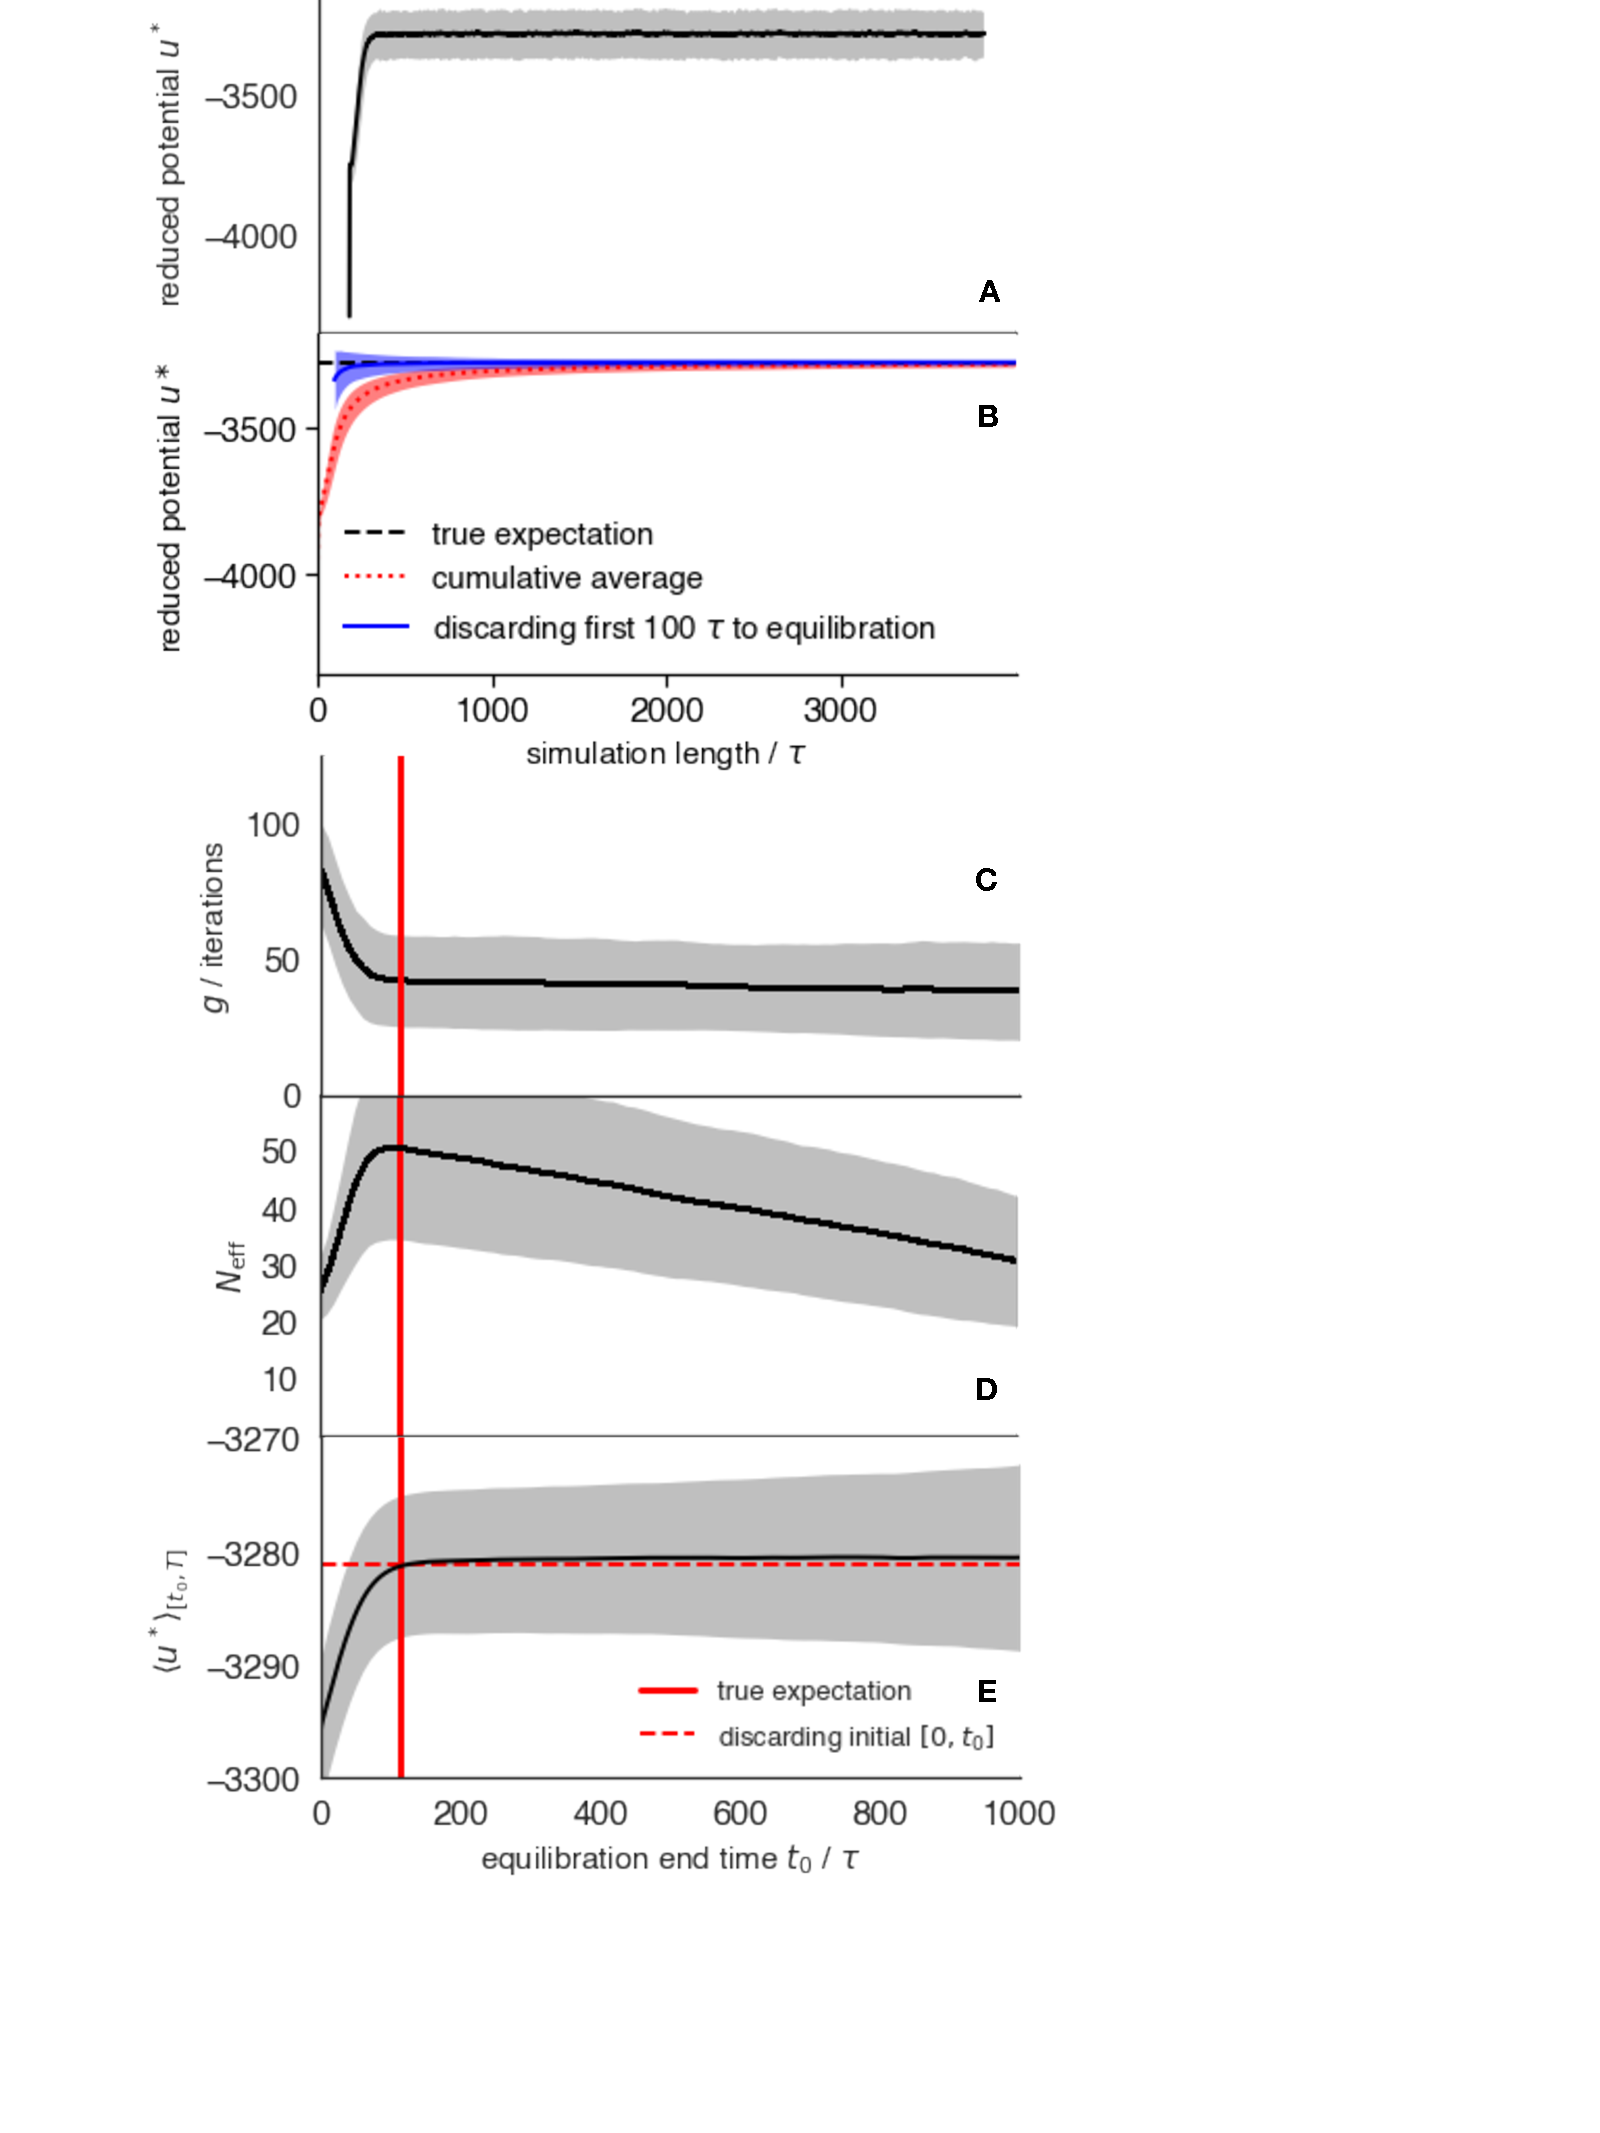
\includegraphics[width=0.95\linewidth]{figures/fig11_equib_detection/Figure.pdf}
    \caption{{\bf Automatic partitioning into equilibration and production regions.}
    (\textbf{A}) The average (black line) standard deviation (shaded region) of the reduced potential $u^*$ over many independent replicate simulations started from the same initial conditions show a significant initial transient change before relaxing to the true average potential energy (\textbf{B}). A cumulative average (red) of the entire simulation data demonstrates simulation bias not seen when initial simulation data is omitted (blue). Using an automated approach to detect equilibration of the boundary $t_0$ using statistical inefficiency $g$ (\textbf{C})  for an effective simulation interval (\textbf{D}). (\textbf{E}) The optimal equilibration boundary $t_0$ is selected to maximize the number of uncorrelated samples.
    \emph{Figure adapted from~\cite{chodera2016simple}.}
    }
    \label{fig:automatic-equilibration-detection}
\end{figure}

To minimize this effect, an initial portion of the simulation is often discarded to \emph{equilibration}~\cite{braun2019best}, with the idea of removing the most heavily biased initial portion of simulation data but retaining the unbiased \emph{production} region that represents a stationary Markov chain process sampling from the desired equilibrium target distribution.
Because the simulation time required for the atypical initial sampler state to relax toward equilibrium is a property of the specific system being simulated and the specific initial conditions selected, it is simplest to collect data for the whole process and use an automated algorithm to select how much data should be discarded to equilibration in a post-processing step.

A simple approach to automatically partitioning simulation data into equilibration and production regions is described in~\cite{chodera2016simple} (illustrated in Fig.~\ref{fig:automatic-equilibration-detection}).
Suppose we have a simulation of length $T$ consisting of correlated data.
Here, the goal of the post-processing step is to select the equilibration boundary $t_0 \in [0, T]$ so as to \emph{maximize} the number of effectively uncorrelated samples remaining in the production region $N_{[t_0,T]}$, which is defined as
\begin{eqnarray}
N_{[t_0,T]} &=& \frac{T - t_0}{g_{[t_0,T]}}
\end{eqnarray}
where $g_{[t_0,T]}$ is the \emph{statistical inefficiency} of a timeseries $a_t$, described in more detail below.
Conveniently, this procedure also produces the information necessary to decorrelate the simulation data for estimating the free energy differences, a requisite next step in analysis.
This approach is implemented within the MBAR~\cite{kylebeauchamp2019choderalab} and alchemlyb~\cite{daviddotson2019alchemistry} packages, and is highly recommended for standard practice.

For additional discussion of working with correlated data and autocorrelation analysis, please refer to the work on Best Practices for Quantification of Uncertainty and Sampling Quality in Molecular Simulations~\cite{grossfield2018best}.

\paragraph{Computing the timeseries for equilibration detection}
Typically, the timeseries of note $a_t$ analyzed in automated equilibration detection is the negative logarithm of the probability density ($\pi(x_t; \vec{\lambda}$)) sampled by the MCMC algorithm (up to an irrelevant additive constant).
For simple independent simulations that sample $x_t \sim \pi(x ; \vec{\lambda})$, this is given by the reduced potential
\begin{eqnarray}
a_t &\equiv& - \ln \pi(x_t; \vec{\lambda}) + c = u(x_t; \vec{\lambda}) .
\end{eqnarray}

Note that the use of the effective reduced potential is not guaranteed to pick up on all slow relaxation processes that may be coupled to the alchemical free energy, but the simplicity of its computation means it is generally appropriate for most cases.

\paragraph{Cautions in automating equilibration detection}
For simulations that are simply not long enough to contain a large number of samples from true equilibrium either because they are very short or contain slow processes, this procedure cannot completely remove the bias.
In such cases, this approach simply selects the final portion of the the simulation, which may be contained in a single substate of configurational space, and may itself lead to biased estimates. 
This situation can be detected if the equilibration boundary $t_0$ is a significant fraction of the total simulation length $T$, with a good rule of thumb being that $T \gtrsim 20 t_0$.
If this is not possible, advanced analysis techniques that assume only local equilibrium (rather than global equilibrium) such as the TRAM estimators~\cite{mey2014xtram,wu2016multiensemble,nuske2017markov} may be more appropriate, but are beyond the scope of this paper. 

\subsection{Decorrelating samples for analysis}
\label{sec:decorrelating-samples}
\paragraph{Computing the statistical inefficiency}
Most estimators require an uncorrelated set of samples from the equilibrium distribution to produce (relatively) unbiased estimates of the free energy difference and its statistical uncertainty.
To do this, the production region of the simulation is generally \emph{subsampled} with an interval approximately equal to or greater than the \emph{statistical inefficiency} $g \ge 1$ to produce a set of uncorrelated samples that can be fed to the estimator machinery~\cite{chodera2016simple},
\begin{eqnarray}
g &\equiv& 1 + 2 \tau_\mathrm{eq} \label{eq:statistical-inefficiency-definition}
\end{eqnarray}
where $\tau_\mathrm{eq}$ is the integrated autocorrelation time, formally defined as
\begin{eqnarray}
\tau_\mathrm{eq} &\equiv& \sum_{t=1}^{T-1} \left(1 - \frac{t}{T}\right) C_t \label{eq:integrated-autocorrelation-time-definition} , 
\end{eqnarray}
with the discrete-time normalized fluctuation autocorrelation function $C_t$ defined as
\begin{eqnarray}
C_t &\equiv& \frac{\expect{a_n a_{n+t}} - \expect{a_n}^2}{\expect{a_n^2} - \expect{a_n}^2} . \label{equation:autocorrelation-definition}
\end{eqnarray}
The basic concept is that $\tau_\mathrm{eq}$ corresponds to the single-exponential decay time for the autocorrelation process that generates samples, so the statistical inefficiency $g$ measures the approximate temporal separation between two effectively uncorrelated samples (where two exponential relaxation times are presumed to be sufficient).

Robust estimation of $C_t$ for $t \sim T$ is difficult due to growth in statistical error, so common estimators of $g$ make use of several additional properties of $C_t$ to provide useful estimates (see \emph{Practical Computation of Statistical Inefficiencies} in~\cite{chodera2016simple} for a detailed discussion).

We recommend using the robust statistical inefficiency computation routines available within the MBAR~\cite{kylebeauchamp2019choderalab} and alchemlyb~\cite{daviddotson2019alchemistry} packages.

\paragraph{Subsampling data to generate uncorrelated samples}
Once the statistical inefficiency $g$ has been estimated, it is straightforward to subsample the correlated timeseries simulation data to produce effectively uncorrelated data that can be fed to the free energy estimators.
Suppose the correlated timeseries is $\{a_t\}_{t=1}^T$; we can form a new timeseries of $N_{\mathrm{eff}} \approx T / g$ effectively uncorrelated samples by selecting a subset of indices $\{ \: t = \mathrm{round}((n-1) \, g) \: | \: n \in \mathrm{range}(1,\ldots ,N) \: \}$ where $\mathrm{round(x)}$ denotes rounding to the nearest integer.

If independent simulations are used, the alchemical state $\vec{\lambda}$ may have a significant impact on the correlation time, and these simulations should be subsampled independently using a separate estimate of the statistical inefficiency $g$ for each alchemical state.
If coupled simulations are used (such as a Hamiltonian replica exchange simulation), the replicas should undergo equivalent random walks in alchemical space, and the replicas can be subsampled with the same $g$ to generate an equal number of uncorrelated samples at each alchemical state.
Conveniently, the approach described above for automated equilibration detection produces an appropriate estimate of $g$ over the production region for automating this process.

\paragraph{Cautions and considerations}
Reliable estimation of the statistical inefficiency is difficult, and estimates will not generally be as precise (in a relative error sense) as averages.
To ensure there is sufficient data available for reliable decorrelation and estimation of free energy differences, it is recommended that the effective number of uncorrelated samples $N_{\mathrm{eff}} \ge \approx 50$ if the BAR or MBAR estimators (discussed below in sec~\ref{subsec:estimators}) are used; the number may need to be much higher with alternate estimators.


\subsection{Uncertainty estimation}
\tocsubsectioncomment{To be split between single/ multiple papers. @Agastya P Bhati/ Peter Coveney to expand. Cycle closure etc. to be moved to second paper.}
\tocsubsectioncomment{@Volunteer: Add discussion of bootstrapping vs t-based confidence intervals for repeats of single calculations (both bad options)?}
\label{subsec:uncertainty}
It is important to consider the variation in your computed free energies from your equilibrium simulations, in order to obtain an estimate of uncertainty of the obtained value for the free energies of interest. A recent Best Practices paper by Grossfield et al.,~\cite{grossfield2018best} provides substantial detail on how to estimate uncertainties from molecular simulations and is a good starting point for this topic. 
The uncertainty of a free energy estimate is limited however, as it is only an estimate of the configurations sampled and cannot contain any information from the phase space not sampled during a simulation. As a consequence, the variance in free energy afforded by any estimator will always be an underestimate of the true uncertainty.
In general, the quantification of different error metrics depends on both data generation and analysis methods used from the ones discussed above. 

The computation of free energies using TI (Sec.n~\ref{subsec:estimators}) is straightforward and the trapezoidal rule is often recommended since it allows unequal spacing of $\vec{\lambda}$ states, which is required to minimize the variance in the free energy estimate, but in principle any good numerical integration method can be used. 
The determination of regions of high curvature when estimating the integral is helpful to determine regions of phase space where more sampling and/or more $\vec{\lambda}$ states are necessary to obtain the best approximation of the integral. Plotting $\vec{\lambda}$ with respect to the gradients at each of the $\vec{\lambda}$ values can be a helpful diagnostic. 
Additionally, computation of the overall variance of TI requires the calculation of the overall variance of integration, rather than each individual $\Delta$G$_{i,i+1}$ and assuming variances add independently. 
Therefore, $\mathrm{var}$($\Delta$f) = $\sum_{i=1}^{K}w_{k}^2 \mathrm{var}(\frac{du}{d\vec{\lambda}})_{k}$.

For alchemical changes that result in smooth, low curvature sets of $\expect{\frac{dU}{d\vec{\lambda}}}$, a relatively small number of $\vec{\lambda}$ states is necessary for sufficient accuracy and low variance in the free energy estimate. 
Depending on the difficulty of the perturbation, the bias introduced by discretization of the integral can become large due to increased curvature, and more $\vec{\lambda}$ intermediate states become necessary to reduce error.
It is recommended that researchers verify that a sufficient number of states are included such that the free energy is essentially invariant to the number of lambda intermediate states chosen. Good heuristics or measures to assess the 'difficulty' of a given perturbation is still an ongoing research topic. 

Compared with TI, the MBAR method (Sec.~\ref{subsec:estimators}) discussed above provides uncertainty estimation directly from solving a set of linear equations to compute the variances between all states. 
The number of states and amount of sampling should be optimized to minimize the uncertainty in the MBAR free energy estimate, while balancing other key considerations such as computational expense. 

If possible, it is advisable to analyze the same set of simulations with different estimators, providing an opportunity for synergy. If different estimators agree the free energy estimate is more reliable than if there are differences between methods that are larger than 1 kcal/mol and would indicate poor convergence. 

Uncertainty can also be assessed for a particular perturbation by repeating calculations with slight changes in initial configurations, forcefield parameters, and different random seeds in the MD engine. 
The assessment of variability in free energy calculations due to repeating simulations has been previously reported~\cite{aldeghi2019accurate,paliwal2011benchmark,mey2016blinded,mey2018impact}, and large variance in free energies estimated from simulations with different random seeds should be flagged as issues with convergence. 

For relative binding free energy calculations, additional sensitivity analysis can be performed by changing the initial configurations of non-core regions of the perturbation topology and determining if this change in configurations results in a large differences in the computed relative free energy, indicating poor sampling of ligand configuration.
The proposed changes in configuration are increasingly relevant if no experimental evidence is available to reduce uncertainty in where the changing atoms should be positioned.

In addition to statistical uncertainty and sampling, a variety of other factors can impact results from binding free energy calculations. In addition to the choice of initial configuration, results can depend on the choice of force field for the protein/receptor, water, and small molecule(s), so rerunning calculations with different choices of force field can also be used to assess how sensitive results and conclusions are to these particular choices. Other factors, like system preparation (choice of protonation state, tautomer, counterion presence, salt concentration, etc.) can also substantially impact results~\cite{mobley2017predicting, mobley2017predictinga}, so unless modelers are confident they have these factors correct, sensitivity to these choices may also need to be examined.

\subsection{Are my simulations any good?}
\label{sec:are-they-good}
There are different easily measurable indicators that can test how well converged simulations are, and if all alchemical states have been sufficiently sampled for a rigorous analysis. Furthermore, once you have established that individual perturbations are well behaved, there are some tricks to ensure the overall perturbation network gives reliable results.

\paragraph{Convergence of simulations}
Fig.~\ref{fig:freeenergytrajectories} illustrates how looking at the convergence of your data may be important. The CB8 host with guest G3 has a longer correlation time than the G6 guest in the octa acid (OA) host. In some cases, slow correlation time may not be expected and therefore not a feature known in advance. To this end, you should always look at all simulation data available and check convergence behaviour for each free energy estimate.
Comparing the free energy trajectories as a function of the simulation time in the forward and reverse time direction is a useful convergence test~\cite{klimovich2015guidelines}.
As shown in Fig.~\ref{fig:freeenergytrajectories}, disagreements larger than 1~$k_{B}T$ in the final part of the forward and reverse trajectories can be useful to detect unconverged results (see also Fig.~\ref{fig:convergence_forward_reverse}).
In this case, one can extend the simulations or try an approach that requires simulations in two separate binding modes where they interconvert at very slow timescales.  
\begin{figure}
    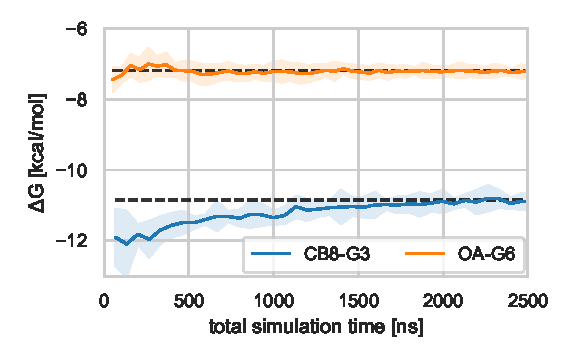
\includegraphics[width=0.90\linewidth]{figures/fig9_convergence/Figure.pdf}
    \caption{Average binding free energy of 5 replicate Hamiltonian replica exchange calculations as a function of total simulation time (i.e. the sum of the simulation time of all replicas) for the two host-guest systems CB8-G3 and OA-G6. Shaded areas represent 95\% confidence intervals around the mean computed from the 5 replicates data. The horizontal dash-dot lines show the final binding free energy prediction of the two calculations after a total of 5230 ns for OA-G6 and 6650 ns for CB8-G3. Dashed lines are the free energy trajectories computed in the forward (blue) and reverse (red) time direction for a single replicate calculation. Longer correlation times in CB8-G3 cause the calculation to converge more slowly. The original data used to generate the plot can be found at \url{https://github.com/samplchallenges/SAMPL6/blob/master/host_guest/Analysis/SAMPLing/Data/reference_free_energies.csv}.
}
    \label{fig:freeenergytrajectories}
\end{figure}

\paragraph{Overlap matrix}
One way of assessing reliability of the calculations is checking the phase space overlap between neighboring $\vec{\lambda}$-windows~\cite{wu2005phasespace, wu2005phasespacea}. For this purpose, a so-called overlap matrix $\mathcal{O}$ can be used. $\mathcal{O}$ is a $K\times K$ matrix, with $K$ being the number of simulated states, i.e. values of $\vec{\lambda}$. Sufficient overlap is important for reweighting estimators such as BAR or MBAR, but cannot help assess reliability of estimates when using TI. 
These matrices are graphical representations of the phase space overlap, i.e. the average probability that a sample generated at state $\vec{\lambda}_{j}$ can be observed at state $\vec{\lambda_{i}}$. As this probability is computed considering the samples from all states, and not just the adjacent states, the values in each row and column add up to 1. In this analysis, the goal is to ensure every state has overlap with its neighbors in both directions, indicated by off-diagonal elements that are sufficiently larger than zero. For accurate calculations, the matrix should be at least tridiagonal.

Details on the calculation and properties of these matrices can be found elsewhere~\cite{klimovich2015guidelines}.
In an overlap matrix $\mathcal{O}$, the off-diagonal values (${O}_{i,j,i\ne j}$) are negatively correlated with the variance of the free energy difference. Accordingly, the uncertainty of the free energy difference between the states $i$ and $j$ will be smaller when ${O}_{i,j,i\ne j}$ is larger (and thus the values in the main diagonal (${O}_{i,j,i=j}$) are smaller). In order to obtain a reliable estimate of the free energy all neighbouring states must be connected, i.e. there must be sufficient overlap between the samples of these states, such that ${O}_{i,j,i\ne j}\ge$ threshold).
However, due to the mathematical derivation it is difficult to explicitly describe the relation of the overlap matrix and the variance by formulae. Consequently, the threshold has to be derived empirically. It has been proposed that the values of the first off-diagonals (i.e. the diagonals above and below the main diagonal) should at least be 0.03 to obtain a reliable free energy estimate~\cite{klimovich2015guidelines}. Smaller values should be considered as a warning sign (see Fig.~\ref{fig:overlap}\textbf{C}), as the variance tends to be underestimated in case of poor overlap.

\begin{figure}
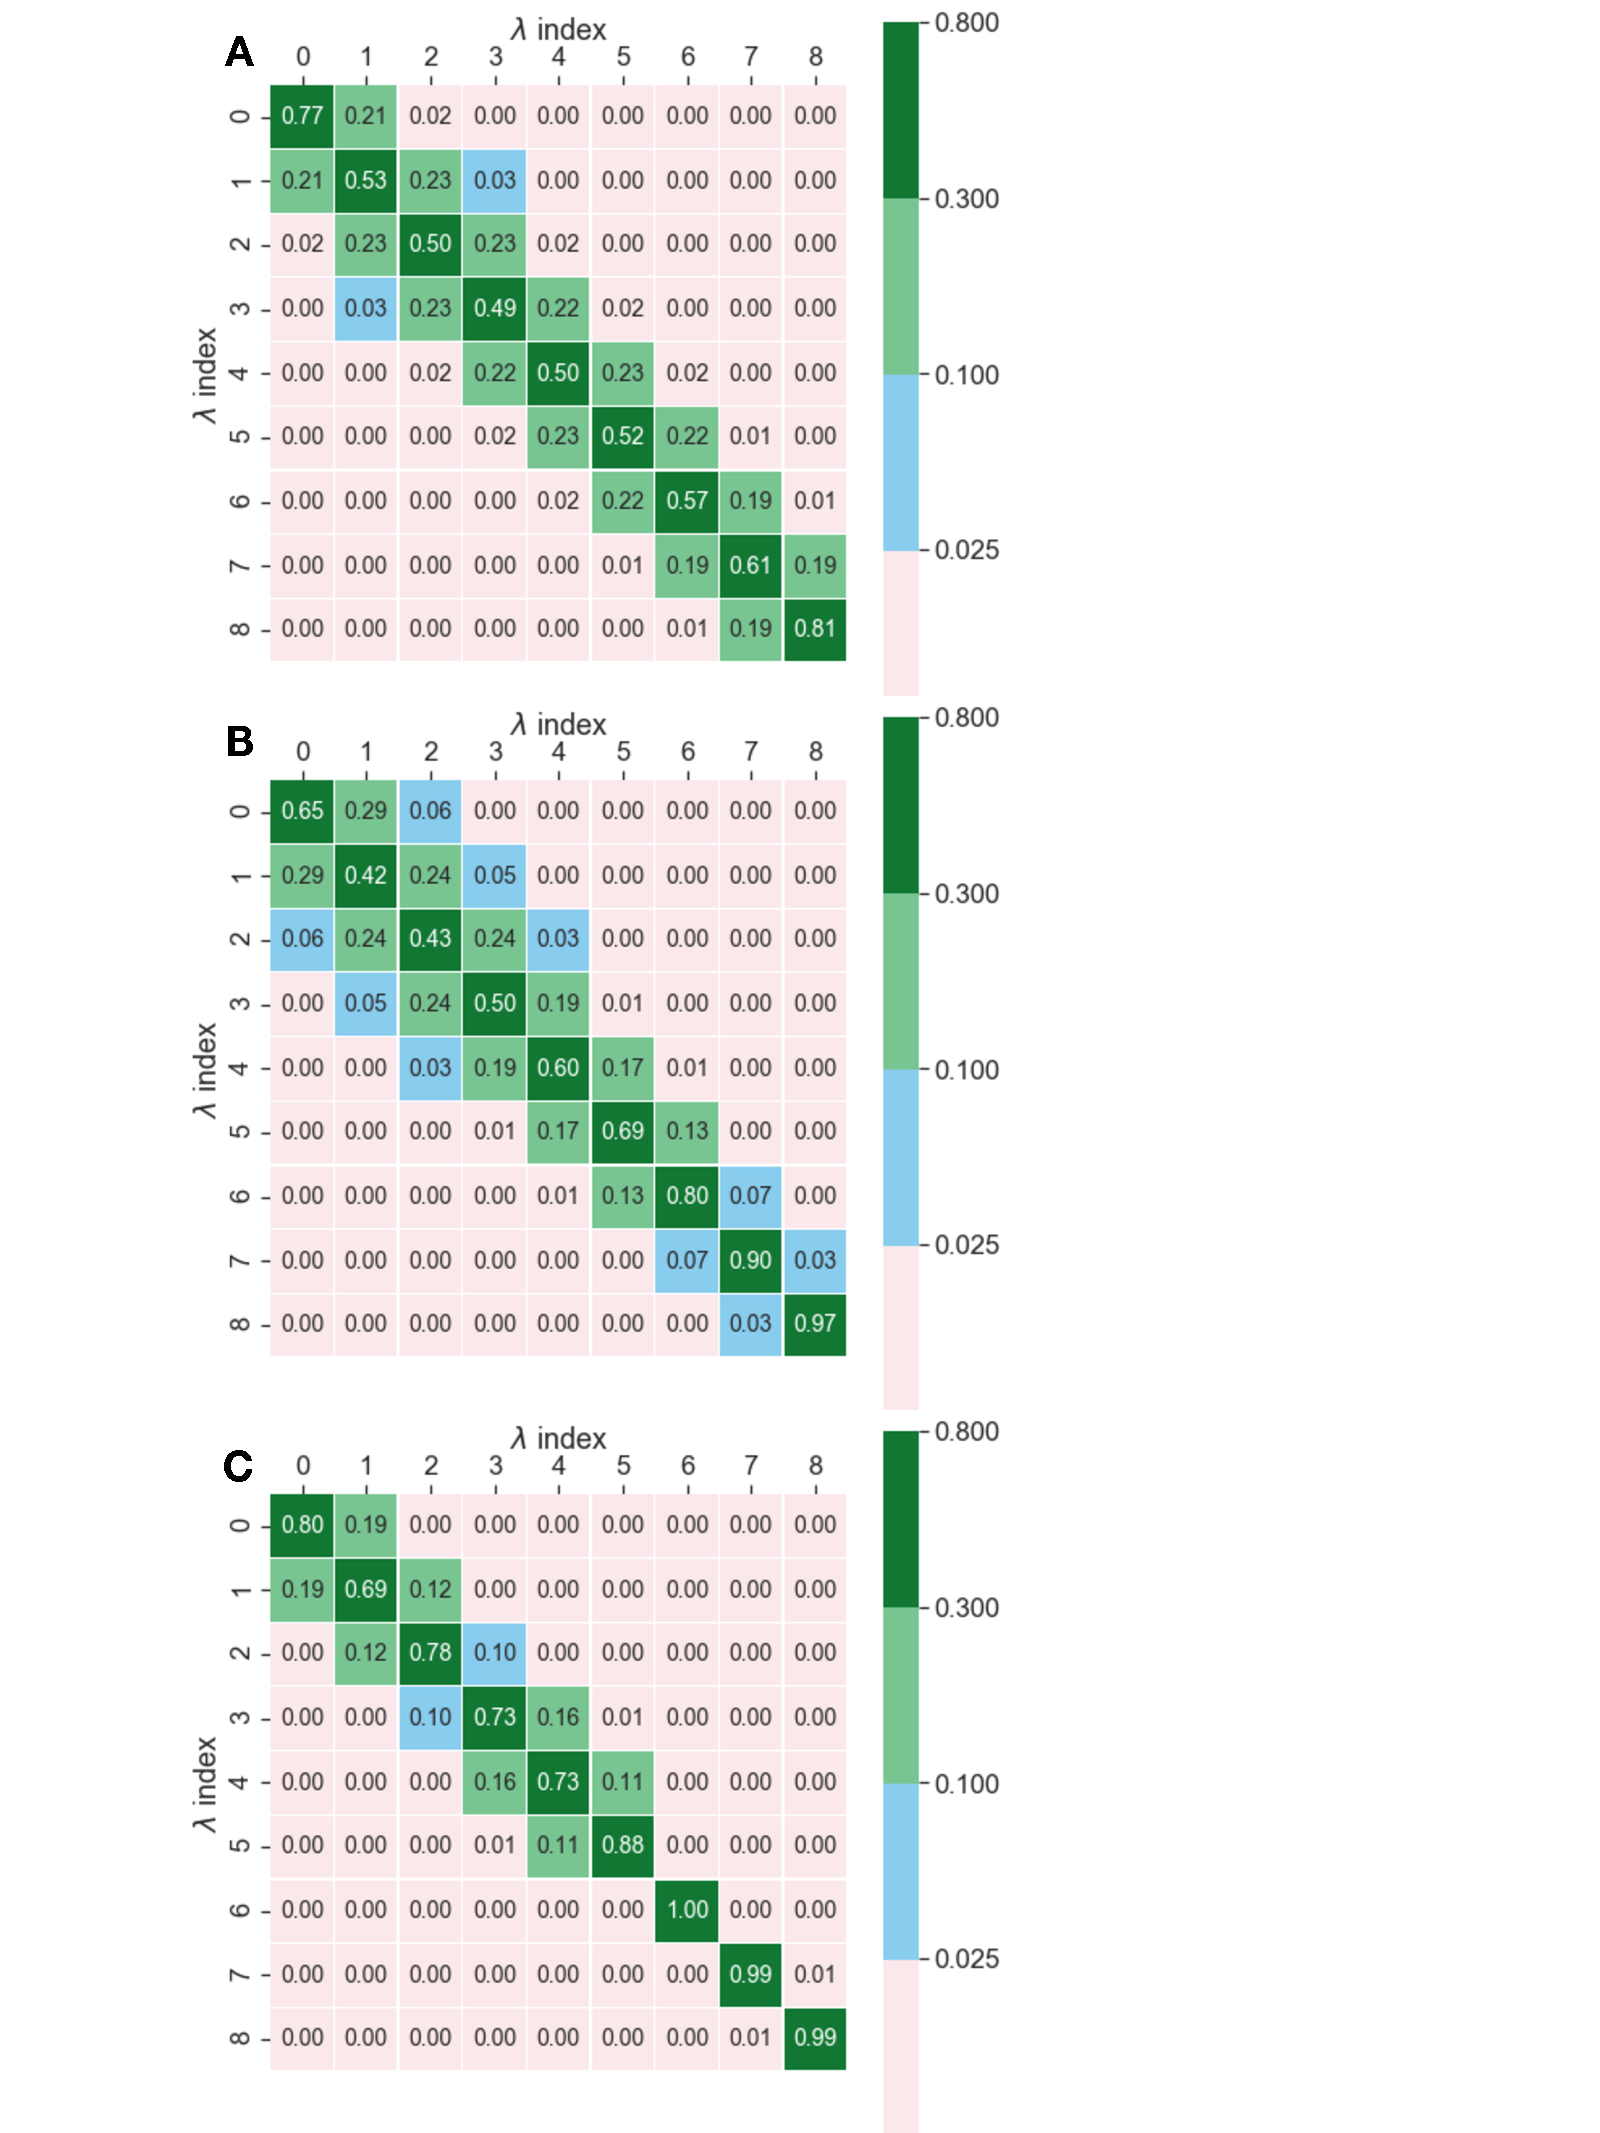
\includegraphics[width=0.90\columnwidth]{figures/fig12_overlap/Figure.pdf}
\caption{\label{fig:overlap} \textbf{Overlap matrices:} Visualising overlap matrices can help with assessing the quality of simulation data. (\textbf{A}) shows good overlap with all first off-diagonal entries well above 0.03, the suggested threshold, (\textbf{B}) is an example of mediocre overlap with good overlap at lower $\vec{\lambda}$ values and poor overlap at high $\vec{\lambda}$ values. (\textbf{C}) shows poor overlap resulting in disconnected simulations with unreliable MBAR estimates.}
\end{figure}

Fig.~\ref{fig:overlap}\textbf{A}, \textbf{B}, and \textbf{C} shows examples of good, mediocre, and poor overlap respectively. For Fig.~\ref{fig:overlap} \textbf{A}, the probability to find a sample from state $i$ in its neighbouring state $j$ is about 0.2 for all states adjacent to the main diagonal, and hence the overall connectivity is good. In the case of Fig.~\ref{fig:overlap} \textbf{B}, the overlap is strongly diminishing in the lower right corner, raising concerns regarding the reliability of the free energy estimate obtained. For Fig.~\ref{fig:overlap} \textbf{C}, the state at $\vec{\lambda}$ index = 6 is connected to neither of its neighbouring states. While this does not necessarily imply that the result for this perturbation is wrong, the energy estimate must at least be considered as highly unreliable.
In order to overcome the issue of poor overlap in this example, additional sampling should be performed by introducing additional states, i.e. $\vec{\lambda}$ values.

Interestingly, as the variance is inversely correlated with the number of states~\cite{klimovich2015guidelines}, it can in principle be reduced below any arbitrary threshold with enough simulation time and a large enough number of $\vec{\lambda}$ windows. However, decreasing the variance to a value close to 0 is not feasible, as this approach would significantly increase the calculation time. While variance can be decreased by increasing simulation length, if the overlap between states is known to be poor, increasing the number of $\vec{\lambda}$ values, or adjusting the spacing of those values to better cover regions of poor overlap will likely provide a larger immediate impact. Different approaches are described in Sec.~\ref{sec:simulation_protocol_choice} and more details can be found in the literature~\cite{dakka2018concurrent, hahn2019alchemical}.

\paragraph{Reversible binding simulations}
An even more stringent test of the correctness of binding free energy calculations is to compare the results to the equilibrium binding constants derived from long timescale reversible binding simulations~\cite{pan2017quantitative}. For small ligands with millimolar affinities, repeated binding to and unbinding from the protein can occur for a large number of times in a sufficiently long unbiased MD simulation (10-100 $\mu$s), and the equilibrium binding constants can be computed from the ratio of bound to unbound fractions of the simulation time. The agreement between the binding free energy calculations and the reversible binding simulations---given the same system preparation and the same force field parameters---will strongly support the correctness of both calculations, as the same results are arrived at by two independent methods, and any discrepancy will suggest some systematic error in one, or both, of the two methods. As part of validation testing of alchemical free energy codes a benchmark set to compare alchemical and direct computation of equilibrium binding constant should become standard in future.

\subsection{Common issues to watch out for during analysis}

It is important to carefully examine output data for common problems. Some of the most important things to check for are:
\begin{itemize}
\item \textbf{Sampling of the binding site by the ligand:} Make sure the ligand samples the binding site reasonably tightly for its expected potency and fit, and that it does not depart out of binding site in the coupled end state if it is a moderate to strong binder. 
\item \textbf{Consistency of free energy estimates across different estimators} Significant discrepancies, meaning results that further outside the mutual error estimates than would be plausible statistically, between free energies calculated with different free energy estimators such as TI, BAR, and MBAR. All of these estimators converge to the same results with sufficient sampling. Differences between them indicate poor overlap or errors in processing.
\item \textbf{Have replicas mixed well?} Poor replica mixing (for replica-exchange) or $\lambda$-space sampling for single-replica methods. If the system is not mixing between states, then the states are insufficiently close for mixing, or else there are bottlenecks in the configurational sampling that limit the accuracy.
\item \textbf{Behaviour of correlation times:} Correlation time that does not vary relatively smoothly as a function of $\vec{\lambda}$. Discontinuities in correlation time with $\vec{\lambda}$ indicate that the system is sampling significantly different configurations with only small changes to the Hamiltonian changes. This usually indicates sampling problems.
\item \textbf{Dependence of the free energy on initial configuration of the system.} Ensemble average properties should not depend on the starting point.
\item \textbf{Torsional sampling} Torsions with multiple low-energy minima where some of these minima are visited rarely or not at all. Which torsions have low energy minima can best be found by comparing to the simulation in the solvent. There should be clear physical reasons that simulation in the complex has different torsional distributions that the ligand in the solvent. 
\item \textbf{Free energy dependence on $\vec{\lambda}$} The free energy difference between states should vary relatively smoothly with $\vec{\lambda}$. If it varies drastically, then either there need to be finer sampling in $\vec{\lambda}$ in this region, or there are sampling problems there.
\item \textbf{Convergence of free energy} The free energy should clearly converge as a function of simulation time (Fig. ~\ref{fig:convergence_forward_reverse}).
\item If using non-equilibrium methods, \textbf{is the result independent of the speed at which the non-equilibrium change is performed}? Non-equilibrium methods are in theory independent of the switching time in the limit of good sampling unless the switching time is simply too short. 
%\item Other Diagnostics for non-equilibrium methods, robustness for switching time etc.?
\item \textbf{Visualization of data} In general, inspect output data such as energies and visualize the simulation trajectories and assess if they match your expectations. Many issues can be spotted by a straight forward visualization. 
\end{itemize}


%%%%%%%%%%%%%%%%%%%%%%%%%%%%%%%
% Conclusions                 %
%%%%%%%%%%%%%%%%%%%%%%%%%%%%%%%
\section{\tocred{Unsettled Practices and Current Limitations}}
\tocsectioncomment{@Everyone to contribute to section on unsettled practices/ current limitiations, as suggested by John Chodera.}
\label{sec:unsettled}

\subsection{Unsettled practices}

\subsection{Current limitations}


%%%%%%%%%%%%%%%%%%%%%%%%%%%%%%%
% Conclusions                 %
%%%%%%%%%%%%%%%%%%%%%%%%%%%%%%%
\section{\tocorange{Conclusions}}
\tocsubsectioncomment{@Volunteer to update reflecting focus on single calculations.}
\label{sec:conclusion}
Alchemical free energy calculations have seen a vast increase in popularity both in academic research as well as pharmaceutical industry applications in structure based drug discovery~\cite{schindler2020largescale, sherborne2016collaborating, wagner2017computational}. Commercial products such as FEP+ and Flare, which provide a convenient user interface make the setup and use of these methods much easier~\cite{wang2015accurate, kuhn2020assessment}, but this convenience comes with less flexibility in terms of choice of simulation protocols. It is also important to understand the current limitations of the methodology to recognise when automated workflow tools can be used effectively for a given protein target and when they are likely to fail still. Prospective prediction challenges such as the Drug Design Data resource grand challenges provide a community driven platform to evaluate different free energy protocols against each other on blinded targets~\cite{gaieb2018d3r, gaieb2019d3r}. Such efforts have highlighted that selection of seemingly identical or similar potential energy function or simulation package does not guarantee production of similar free energies owing to differences in simulation protocols. 
We hope that the best practice guide provides a set of tools that allow a better understanding of how to setup, run, and reliably interpret alchemical free energy calculations. 

%%%%%%%%%%%%%%%%%%%%%%%%%%%%%%%
% Software                    %
%%%%%%%%%%%%%%%%%%%%%%%%%%%%%%%
\section{\tocorange{Selection of available software packages}}
\tocsectioncomment{@Volunteers to update.}

\label{sec:software}
There are many different software solutions available for the setup, running, and analysis of alchemical free energy calculations. These will vary in customizability and ways in which they are ran, e.g. graphical user interface versus command line tool or python script. The following provides a non-exhaustive list of commercial and noncommercial tools available for conducting alchemical free energy calculations. 
\begin{itemize}

\item [] \textbf{Simulation software: Commercial}
   \begin{itemize}
    \item \href{https://www.schrodinger.com/fep}{FEP+} is a tool offered by Schr\"{o}dinger Inc. under a commercial license. It has an intuitive GUI which makes it easier for non-experts to run alchemical free energy calculations and analyze the results. It runs the DESMOND MD package under the hood and hence parallelizes well on GPUs~\cite{wang2015accurate}. 
    \item \href{https://www.cresset-group.com/software/flare/}{Flare} is a commercial structure-based drug design software offered by Cresset. Similar to FEP+ it has an easily accessible graphical user interface and strives to facilitate free energy calculations for non-experts while offering advanced users full control via a Python API. It only runs on GPUs, using CUDA or OpenCL~\cite{kuhn2020assessment}. It is build on top of the open source software packages Sire and BioSimSpace (cf. below).
    \item The molecular operating environment (\href{https://www.chemcomp.com/Products.htm}{MOE}) offered by the Chemical Computing Group (CCG) has a tool for performing free energy calculations. It is built on AMBER-TI (cf. below).
    \end{itemize}
    \item[]All the above tools also provide a convenient setup and analysis suite and are really a one in all product. \newline
\item [] \textbf{Simulation software: Free/low cost academic and Commercial}
	\begin{itemize}
	\item \href{https://www.charmm.org/}{CHARMM} has a variety of tools developed over the years. The PERT module can be used to define initial and final states and define the intermediate lambda points. FREN and BAR modules can be used to analyze the data after the MD run. Lambda-dynamics-based free energy calculation can be carried out using the BLOCK module.  
	\item \href{https://ambermd.org/}{AMBER}, including its new pmemd.cuda version supports free energy calculations~\cite{salomon-ferrer2013overview}. 
	\item \href{http://www.gromos.net/}{GROMOS} offers an extensive and flexible molecular dynamics and simulations analysis suites with free energy calculation functionalities including customizable alchemical paths and various sampling protocols~\cite{schmid2012architecture, kunz2012new, eichenberger2011gromos}.
	\end{itemize}
\item [] \textbf{Simulation software: Open Source}
	\begin{itemize}
	\item \href{https://www.plumed.org/}{PLUMED} is a tool which enables the usage of a variety of MD engines. It is designed as a plugin for MD packages such that it analyzes the trajectory on the fly. It also offers a VMD based plugin for the computation of collective variables~\cite{bonomi2019promoting}.   	
	\item \href{https://biosimspace.org/}{BioSimSpace} is a multiscale molecular simulation framework, written to allow computational modellers to quickly prototype and develop new algorithms for molecular simulation and molecular design~\cite{hedges2019biosimspace}. 
	\item \href{https://siremol.org/}{Sire} is a multiscale, molecular simulation framework that provides several applications, including SOMD, an MD/MC code for performing FEP calculations via an interface to OpenMM. 
	\item \href{http://getyank.org/latest/index.html}{YANK} is a tool developed by John Chodera and group on the top of OpenMM MD package. It allows the users to write their inputs in easy-to-use YAML format.
	\item \href{http://www.gromacs.org/}{GROMACS} is a molecular simulation package with a significant number of free energy methods implementations. The LiveCOMS GROMACS tutorial includes an example free energy calculation~\cite{lemkul2018From}.
	\item \href{http://pmx.mpibpc.mpg.de/instructions.html}{PMX}, an add-on to GROMACS, offers a mutation free energy calculation module~\cite{abraham2015gromacs}.
	\item \href{https://github.com/qusers/Q6}{Q} is MD code for performing FEP calculations using a variety of force fields~\cite{aaquist2017q6}. 
	\end{itemize}
\item[] \textbf{Setup tools:}
	\begin{itemize}
	\item \href{http://pmx.mpibpc.mpg.de/instructions.html}{PMX}: Setup of perturbation maps, perturbed topologies and input coordinates for GROMACS simulations at \url{https://github.com/deGrootLab/pmx}.
	\item \href{https://github.com/MobleyLab/Lomap}{Lomap/Lomap2} : Relative alchemical transformation graph planning for setting up perturbation networks~\cite{liu2013lead}.
	\item \href{http://www.charmm-gui.org/}{CHARMM-GUI} is a web-based tool for setting up a variety of MD simulations. It can be used to generate CHARMM scripts for solvation and ligand-binding free energy calculations~\cite{jo2008charmmgui}.
	\item \href{https://github.com/qusers/qligfep}{QligFEP} offers robust and fast setup of FEP calculations for the software package Q~\cite{jespers2019qligfep}.
	\item \href{https://github.com/protocaller/ProtoCaller}{ProtoCaller}, a setup tool for the automation of Gromacs free energy calculations~\cite{suruzhon2020protocaller}.
	\item \href{https://fesetup.readthedocs.io/en/latest/introduction.html}{FESetup} has been developed primarily to setup calculations in AMBER, GROMACS and SIRE~\cite{loeffler2015fesetup}.
	\end{itemize}
\item []\textbf{Analysis tools:}
	\begin{itemize}

	\item Alchemlyb: Multipackage free energy analysis
	\url{https://github.com/alchemistry/alchemlyb}~\cite{daviddotson2020alchemistry}.
	\item pymbar: MBAR implementation, but have to roll your own analysis wrapper      
	\url{https://github.com/choderalab/pymbar} \cite{shirts2008statisticallya}.
	\item Arsenic: Standardising alchemical free energy analysis \url{https://github.com/openforcefield/Arsenic}
	\item Free Energy Workflows: Sire-specific free energy map analysis using weighted path averages \url{https://github.com/michellab/freenrgworkflows}.
	\end{itemize}
\item[] Generally, commercial software will offer more complete pipelines in which standalone analysis applications are not necessarily needed; free and open source packages often require manual analysis but allow more flexibility and modification.
\end{itemize}


\section{\tocorange{Checklist}}
\tocsectioncomment{@Volunteer to update checklists/ move relevant sections to second paper.}
\label{sec:checklist}
\begin{Checklists*}
\begin{checklist}{ Know what you want to simulate}
    \textbf{Initial questions you should ask before you set up an alchemical free energy calculation using molecular dynamics simulations}
\begin{itemize}
    \item Do I understand the biology, chemistry and physics of my system?
    \item Have I properly prepared my protein and ligand systems?
    \item Does my system contain any structures that require custom parameters?
    \item What simulation protocol will provide the most evidence to verify my hypothesis?
    \item Are the projected computational expense and runtime realistic for my scientific goals?
    \item Will my protocol be reproducible? 
    \item Will my statistics be reliable? If not, would more replicates solve the problem? 
    \item Can I open-source my data?
\end{itemize}
\end{checklist}

\begin{checklist}{Preparing your simulations}
\textbf{Steps to getting started setting up your alchemical free energy calculation}
\begin{itemize}
    \item Make sure you know why you have picked your (combination of) force field(s)
    \item Energy minimize your system
    \item Equilibrate your system properly with your choice of thermodynamic ensemble
    \item Check the stability of your system and whether it behaves the way you believe it should
\end{itemize}
\end{checklist}

\begin{checklist}{Running absolute simulations}
        \textbf{Steps to running your absolute alchemical free energy calculations}
\begin{itemize}
 \item Check your ligands have the same, biologically correct binding pose
        \item Make sure your \textlambda-scheduling is  appropriate
        \item Check if your ligands are discharging and decoupling correctly
        \item Set up your restraints correctly
        \item Make sure you subsample the data in your free energy estimation protocol
        \item Apply the appropriate correction terms
\end{itemize}
\end{checklist}

\begin{checklist}{Running relative simulations}
        \textbf{Steps to running your relative alchemical free energy calculations}
\begin{itemize}
   \item Check your ligands  have the same, biologically correct binding pose
        \item Make sure your $\lambda$-scheduling is set correctly
        \item Make sure your molecular transformations are realistic (1-5 heavy atoms for reliable computations)
        \item Generate a perturbation network by your method of choice; check whether you have enough cycle closures to check consistency in the results
        \item Check whether dummy atoms were assigned correctly
        \item Consider subsampling the data in your free energy estimation protocol
        \item Apply the 
        appropriate correction terms
\end{itemize}
\end{checklist}
\end{Checklists*}

%Analyis checklist
\begin{Checklists*}
\begin{checklist}{How do I know which simulations are unreliable?}
    \textbf{Situations suggesting your relative alchemical free energy calculations have not run properly (assuming absence of experimental affinities)}
        \begin{itemize}
                \item Standard error (\textsigma) should not be \textgreater1 kcal·mol$^{-1}$ 
    \item Simulated systems have not converged - trajectories should be manually checked for consistency; other methods such as generating RMSD plots are also recommended
    \newline\newline\textit{Relative:}
    \item If you observe hysteresis in perturbations and incorrect cycle closures
    \item Energy differences \textgreater$\sim$15 kcal$\cdot$mol$^{-1}$  are likely unreliable
    \newline\newline\textit{Absolute:}
    \item Energies \textless$\sim$-15 kcal$\cdot$mol$^{-1}$  are likely unreliable
    \item The ligand has not sampled most of the intended region after the decoupling step
    \item The ligand is drifting out of the intended region after the decoupling step
        \end{itemize}
\end{checklist}

\begin{checklist}{Why are they not reliable?}
    \textbf{Suggestions for finding out why your alchemical free energy calculations may not be reliable}
\begin{itemize}
    \item Check again whether dummy atoms were assigned correctly
    \item Inspect the trajectories across the $\lambda$-schedule (particularly the endpoints) for problems described in the text
    \item Inspect the overlap matrices for lack of overlap
\end{itemize}
\end{checklist}

\begin{checklist}{Data Analysis}
    \textbf{Steps to analyzing your output data correctly}
\begin{itemize}
    \item Make sure you have run enough replicates to ensure statistical reliability (\textgreater3)
    \item Compute both correlation and ranking coefficients and ranking statistics (e.g. r, \textrho, MUE and \texttau)
    \item Include error bars in all your visual analyses
\end{itemize}
\end{checklist}
\end{Checklists*}
\clearpage


\section*{Author Contributions}
%%%%%%%%%%%%%%%%
% This section mustt describe the actual contributions of
% author. Since this is an electronic-only journal, there is
% no length limit when you describe the authors' contributions,
% so we recommend describing what they actually did rather than
% simply categorizing them in a small number of
% predefined roles as might be done in other journals.
%
% See the policies ``Policies on Authorship'' section of https://livecoms.github.io
% for more information on deciding on authorship and author order.
%%%%%%%%%%%%%%%%
\textbf{ASJSM}: Coordinated the document, contributed to most sections, and co-designed Figs.~\ref{fig:fig_binding_thermodynamic_cycle},~\ref{fig:fig_topology},~\ref{fig:fig_mcss},~\ref{fig:fig_types_of_networks},~\ref{fig:fig_absolute_thermodynamic_cycle},~\ref{fig:scatterplot_analysis}, and created Figs.~\ref{fig:fig_what_is_lambda},~\ref{fig:fig_what_is_alchemy},~\ref{fig:overlap},~\ref{fig:pmf} and replotted~\ref{fig:automatic-equilibration-detection} and~\ref{fig:fig_types_of_networks}.\\
\textbf{BA}: Helped write the uncertainty estimation, stopping conditions, and output analysis sections and created figure ~\ref{fig:convergence_forward_reverse}.\\
\textbf{HBM} Contributed to Sec.~\ref{sec:plot_data} and Fig.~ \ref{fig:scatterplot_analysis} and helped edit the paper.\\
\textbf{JDC}: Wrote Sec.~\ref{sec:decorrelating-samples} and~\ref{sec:automatic-equilibration-detection} discussed structure and design of the whole document, suggested Figs.~\ref{fig:fig_what_is_alchemy} and~\ref{fig:fig_sampling_scheme}. \\
\textbf{DFH} Contributed to Sec.~\ref{sec:software} and helped edit the paper. \\
\textbf{MK}: Contributed to Sec.~\ref{sec:data_analysis}, provided the data for figure~\ref{fig:overlap}, compiled the dataset for Sec.~\ref{sec:benchmark} and helped edit the paper.\\
\textbf{JM}: Contributed to Sec.~\ref{subsec:reproducible},~\ref{sec:prerequisites},~\ref{sec:important_path},~\ref{subsec:estimators},~\ref{subsec:uncertainty}, and~\ref{sec:conclusion}\\
\textbf{DLM}: Contributed to the outline, drafted some of the sections, gave ideas on figures, and helped edit the paper.\\
\textbf{LNN}: Helped write the simulation length, stopping conditions, and information saving section. Edited and reviewed alchemical path section.\\
\textbf{SP} Wrote Sec.~\ref{sec:software}. \\
\textbf{AR}: Created figure~\ref{fig:freeenergytrajectories}, contributed to sections~\ref{sec:theory} and~\ref{sec:simulation_protocol_choice}, and helped edit the paper.\\
\textbf{JS}: Created Figs.~ \ref{fig:fig_what_is_alchemy},~\ref{fig:fig_binding_thermodynamic_cycle},~\ref{fig:fig_topology},~\ref{fig:fig_mcss},~\ref{fig:fig_absolute_thermodynamic_cycle},~\ref{fig:scatterplot_analysis}, and an initial draft of~\ref{fig:fig_types_of_networks}. Wrote Sec.~\ref{sec:plot_data}, the checklist Sec.~\ref{sec:checklist}, and contributed to general formatting discussions and editing.\\
\textbf{MRS}: Helped create figure~\ref{fig:fig_what_is_lambda}, wrote Sec.~\ref{sec:important_path} describing choices for alchemical pathways and parts of~\ref{sec:data_analysis} on the analysis for free energy calculations. Reviewed and edited text throughout.\\
\textbf{GT}: Contributed to Sec.~\ref{sec:intro} and~\ref{sec:drugdiscovery}, and helped edit the paper.\\
\textbf{HX}: Contributed Sec.~\ref{subsec:accuracy}, to Sec.~\ref{sec:relative-fe-protocol}, and to Sec.~\ref{sec:are-they-good}.
% We suggest you preserve this comment:
For a more detailed description of author contributions,
see the GitHub issue tracking and changelog at \githubrepository.

\section*{Other Contributions}
%%%%%%%%%%%%%%%
% You should include all people who have filed issues that were
% accepted into the paper, or that upon discussion altered what was in the paper.
% Multiple significant contributions might mean that the contributor
% should be moved to authorship at the discretion of the a
%
% See the policies ``Policies on Authorship'' section of https://livecoms.github.io for
% more information on deciding on authorship and author order.
%%%%%%%%%%%%%%%
Julia E. Rice participated in the original discussion of the document at the Best Practices in Molecular Simulation Workshop Hosted by at NIST, Gaithersburg, MD, August 24th-25th, 2017.
Marieke Schor proofread the manuscript. 

% We suggest you preserve this comment:
For a more detailed description of contributions from the community and others, 
see the GitHub issue tracking and changelog at \githubrepository.


\section*{Potentially Conflicting Interests}
%%%%%%%
%Declare any potentially competing interests, financial or otherwise
%%%%%%%
JM is a current member of the Scientific Advisory Board of Cresset. 
MK is employed by Cresset who commercially distribute a software for performing alchemical free energy calculations. MRS is a Open Science Fellow and consultant for Silicon Therapeutics.
JDC is a current member of the Scientific Advisory Board of OpenEye Scientific Software and a consultant to Foresite Laboratories.
\section*{Funding Information}
%%%%%%%
% Authors should acknowledge funding sources here. Reference specific grants.
%%%%%%%
ASJSM and JM acknowledge funding through an EPSRC flagship software grant: EP/P022138/1
MK and JM acknowledge funding through Innovate UK by KTP partnership 011120.
AR acknowledges partial support from the Tri-Institutional Program in Computational Biology and Medicine and the Sloan Kettering Institute.
HEBM acknowledges support from a Molecular Sciences Software Institute Investment Fellowship and Relay Therapeutics.
DLM acknowledges support from the National Institutes of Health (R01GM108889, R01GM124270, and R01GM132386), and the National Science Foundation (CHE 1352608).
JDC acknowledges support from the National Institutes of Health (NIH P30 CA008748, NIH R01 GM121505, R01 GM132386).
A complete funding history for the Chodera lab can be found at \url{http://choderalab.org/funding}.
The content is solely the responsibility of the authors and does not necessarily represent the official views of the National Institutes of Health.

\section*{Author Information}
\makeorcid
\bibliography{alchemical,manual}

%%%%%%%%%%%%%%%%%%%%%%%%%%%%%%%%%%%%%%%%%%%%%%%%%%%%%%%%%%%%
%%% APPENDICES
%%%%%%%%%%%%%%%%%%%%%%%%%%%%%%%%%%%%%%%%%%%%%%%%%%%%%%%%%%%%

%\appendix


\end{document}
